\documentclass[11pt,letterpaper]{article}
\usepackage[utf8]{inputenc}
\usepackage[english, activeacute]{babel}
\usepackage{lscape}
\usepackage{graphicx}
\usepackage [round]{natbib}
\usepackage{float}
\usepackage{subfig}
\usepackage{amsmath,
            amsfonts,
            amssymb}
\usepackage{graphicx}
\usepackage{minted}
\usepackage{hyperref}
%
%
%%%%%%%%%%%%%%%%%%%%
\def\bibfont{\fontsize{11}{12}\selectfont}
%----------------------------------

\title{ \textbf{Topographic Effects in Seismic Engineering Based Upon a Rational Approach}}
%

\author{Xxxxxx Yyyyyy Wwwwww Zzzzzzz\footnote{Universidad EAFIT, Departamento de Ingeniería Civil. Medellín, Colombia}}
              
\date{} 

\newcommand\frontmatter{%
    \cleardoublepage
  %\@mainmatterfalse
  \pagenumbering{roman}}

\newcommand\mainmatter{%
    \cleardoublepage
 % \@mainmattertrue
  \pagenumbering{arabic}}




%\title{\textbf Topographic Effects in Seismic Engineering Based Upon a Rational Approach}
%\date{}
%\author{Xxxxxx Yyyyyy Wwwwww Zzzzzzz}

\usepackage{cleveref}
\begin{document}

\hypersetup{linktocpage}

\setlength{\parskip}{6pt}
\setlength{\baselineskip}{18pt}
\setlength{\parindent}{0.25in}

\cleardoublepage
\thispagestyle{empty}

\begin{center}

{\huge 
\textbf{Topographic Effects in Seismic Engineering Based Upon a Rational Approach\\}}

\vspace{50pt}
{\Large Committee Members:\\
\vspace{10pt} 
\textbf{Dr. Juan Diego Jaramillo (Chair)}\\ 
\textbf{Dr. Francisco Sanchez-Sesma}\\ 
\textbf{Dr. Juan Gomez }\\ }

\vspace{50pt}
{\Large PhD Candidate:\\
\textbf{Xxxxxx Yyyyyy Wwwwww Zzzzzzz}\\}
\vspace{-5pt}
msaenz@eafit.edu.co


\vfill
{\Large A dissertation Submitted to the\\
Faculty of the School of Engineering of\\
Universidad EAFIT\\
 in partial fulfillment of the requirements for the degree of\\
 Doctor of Philosophy\\
%Departamento de Ingeniería Civil\\
%Universidad EAFIT\\
%Medellín, Colombia\\
2018}

\end{center}

\cleardoublepage
\phantomsection
\tableofcontents % indice de contenidos

\cleardoublepage
\phantomsection
\addcontentsline{toc}{section}{LIST OF FIGURES}
\listoffigures % indice de figuras


\cleardoublepage
\phantomsection
\addcontentsline{toc}{section}{LIST OF TABLES}
\listoftables % indice de tablas
\newpage

\mainmatter

\maketitle


\abstract{Site effects in ground response analysis are the result of the combined contribution between mechanical impedance and the geometry of the surface and sub-surface topography. While seismic codes are provided with methods to account for the mechanical effect, the topographic aggravation remains practically untreated by the practicing community. One of the challenges for its consideration in terms of simplified approaches lies in the fact that many specific problem parameters are involved. A  natural alternative is to make of use modern numerical simulation algorithms, however a highly detailed model requires large computing resources and field data which is scarce for the practicing engineer. In this work we use a conceptual and rational approach to address geometric effects and particularly to identify controlling parameters even under realistic scenarios. To put some practical perspective into the work we start with the dynamic analysis of the Aburrá valley region in Medellin-Colombia where we show that topographic aggravation can be due to a localized or isolated irregularity or to the more complex scenario of various interacting features. By proposing an alternative partition of the field and the concept of topographic resolution we derive a method to generate simplified models to capture geometric effects by standard numerical algorithms. The model however has a limited resolution in terms of the response spectra as it uses a target structural period to decide what structural features are relevant in the model.}
\newpage

%%%%%%%%%%%%%%%%%%%%%%%%%%%%%%%%%%%%%%%%%%%%%%%%%%%%%%%%%%%%%%%%%%%%%%%
%%%% %%%%%%%%%%%%%%%%%%%%%%%%I N T R O D U C C I O N%%%%%%%%%%%%%%%%%%%%%%%%%%%%%%%
%%%%%%%%%%%%%%%%%%%%%%%%%%%%%%%%%%%%%%%%%%%%%%%%%%%%%%%%%%%%%%%%%%%%%%%

\section{Introduction}
\subsection*{Preliminary}
\addcontentsline{toc}{subsection}{Preliminary}

It is a known fact, as various numerical and experimental studies show \citep{trifunac1971analysis, bouchon1996seismic} that the response at a local site is due to the combined effect of the material properties as well as to the surface and sub-surface topography. While the first of these two problems may be considered well understood, the topographic effect still lacks a consolidated approach that can be followed by practicing professional engineers.

The mechanical effect has a long history of study by the academic and engineering community, to the extent that in seismic codes it can be considered through approaches based upon models with different levels of sophistication. In the simplest techniques the prescribed bedrock motions are modified by site coefficients, which typically, are a function of the mechanical properties of the last $30$ meters of the soil deposit. This simplistic approach implicitly considers vertical incidence of the wave field and a one-dimensional propagation model in which the site is assumed to be conformed by a horizontally-infinite stack of layers. In a next level of refinement there are methods where the one-dimensional wave propagation analysis is extended to consider also nonlinear response, although using equivalent linear techniques where the inelastic soil properties are taken into account in terms of modulus reduction and damping ratio curves \citep{shnabel1972shake, lysmer1975flush}.

In contrast with the mechanical problem, the possibility of including geometric effects in site response analysis methods is still the sole domain of researchers and academicians as there are only a few codes \citep{bard1995guidelines, code2005eurocode} with simplified procedures to address topographic aggravation. As concluded, from mostly theoretical works \citep{ashford1997topographic, geli1988effect, Trifunac1973, [1971]TRIFUNAC, sanchez-sesma91, sanchez1979ground, tsaur2008analytical}, the main signature of the geometric effect on the ground response is a spatial variability in the resulting displacements. Interestingly, although the spatial variation of the motion implies a frequency dependence of the problem, the few available code-based approaches use frequency independent amplification functions to be imposed upon the bedrock motions and dependent on geometric parameters of the site.

Although there have been important advances in the theoretical study of topographic effects, most of the available works have focused on the response of simple isolated topographies \citep{[1990]Sz, [1985]Sz, boore1972note, [1991a]TodyLee}. Despite the fact that these contributions have been instrumental in providing conceptual understanding to the causes of the perturbations experienced by the incident motions as they interact with geometric irregularities, such idealized scenarios are far away from being realistic. It is relatively straightforward to estimate the amplification factor in the case of an isolated hill in a half-space if one knows the internal angle of the hill and its characteristic dimensions. However, a more realistic topographic scenario is expected to be conformed by several hills and canyons of varying characteristic dimensions and with different levels of interaction.

Clearly, the prediction of the spatial variations in the resulting surface motions under these challenging conditions constitutes a difficult engineering problem posing several questions still unresolved. For instance there are no clear guidelines about the minimum geometric parameters that must be included in a numerical model for site effects or what is the influence of the large scale topography in the response at local site.

Following the current growth in computing power and the proliferation of robust numerical algorithms, one potential alternative is to use highly detailed computational models \citep{Akcelik2003, Bielak2005, bielak2003, restrepo2012three, restrepo2016effects, Taborda2013, Taborda2011}. However, robust numerical simulations require field data that is rarely available at the practicing level and thus are still far from being applicable by the engineering community. In fact there are only a few works reporting the use of such models to conduct site response analysis and mostly of academic interest, \citep{makra2016site, assimaki2004topography}.

This ongoing research effort is devoted to the construction of simplified models and methods intended to capture topographic effects on site response analysis under realistic scenarios.  In particular, we address the question of whether results based upon simplified models, built with limited field data, are of any use for engineering purposes or, if on the contrary, the effects of topography on the ground response are necessarily constraint to be treated by academic and research scientists.

\subsection*{What is novel in this research?}
\addcontentsline{toc}{subsection}{What is novel in this research?}

Most of the available theoretical works dealing with topographic effects focus primary in the analysis of isolated topographies like hills, canyons or ridges. Although the study of these fundamental shapes contribute to the conceptual understanding of the problem and help elucidate the physics of the involved phenomena, these cases are highly idealized and distant from realistic conditions. In fact, a larg number of urban areas are located within scenarios conformed by a combination of concave and convex topographic features of length scales varying across a wide range of characteristic dimensions. These limitations are also reflected in the few available seismic design regulations considering topographic effects as they provide modification factors which are frequency independent neglecting the size effect existing in the geometric irregularity.

In this work we refer to the more realistic scenario conformed by a combination of irregularities interacting between them as the {\bf coupled} or regional scenario. This idea leads to a natural question: ¿ what is the required level of resolution that must be included in a model intended for ground  motion prediction in earthquake engineering? In other words, ¿ what specific details of the surface topography need to be considered when conducting site response analysis coupled to topographic effects?

In this dissertation we study topographic effects under coupled scenarios. Even though we start from a single fundamental topographic feature we extend the analysis to consider the interaction between coupled shapes. As a novel ingredient, not considered before, we bring into the problem a target frequency (or target structural period) originated in the fact that site response analysis is conducted as an input for seismic resistant design. This idea suggests that the level of topographic refinement depends upon the purpose of the analysis. 



\subsection*{Scope of research}
\addcontentsline{toc}{subsection}{Scope of research}
This research proposal is intended to the development of simplified methods of analysis for the consideration of topographic effects in site response prediction under realistic scenarios, consisting of local sites embedded in complex regional topographies. Our proposed approach has been termed rational as it starts from the analysis of fundamental topographies and identifies controlling factors that are later used in an alternative partition of the total field. This idea is basically the extension of the superposition method commonly used in the solution of problems found in the classical theory of elasticity. In this superposition effort we identify as the natural starting point the problem of horizontally polarized $SH$-waves as in this case the solution can be separated into a geometrical and a diffracted component with this last term admitting an analytic solution. As a result of this rational method of analysis we have managed to solved problems of relative geometric complexity. Although the study of topographic effects with scalar models is very limited, the conceptual aspects identified in this simple case are later used as analysis tool in the case of more realistic in-plane problems.

We introduce the concept of a topographic element as the fundamental building block in terms of which the analyst can build an arbitrary topographic profile. Essentially, following the same approach in which one uses the maximum frequency of the incident field to define the appropriate element size in a numerical simulation of a wave propagation problem, here we use a target analysis frequency to select the appropriate level of topographic resolution. The target frequency is related to the range of structural periods for which the site effects analysis is conducted in the first place. As a consequence, the final model includes only the topographic information that is required for that specific analysis resulting in a simplified model. 

To study the impact in the response of the different levels of simplification in a given model we use the level of topographic resolution (associated to the size of the topographic element). Accordingly, if a surface topography is understood as a series of geometric singularities of varying length-scale (or wavelength) then, a highly detailed model is one with singularities of small characteristic dimensions. Similarly, a poorly approximated topography is one in which all singularities whose characteristic dimension is smaller than a prescribed threshold are smoothed out. This concept of topographic resolution level appears naturally following the contribution from \cite{jaramillo2013analytic} where it is recognized that the main controlling factor of the spatial variation of the ground motion corresponds to geometric singularities existing in the topographic profile. Here we analyze models with different levels of resolution using an approach based on the response of a simple semi-infinite wedge and leading to a systematic way of approximating a given topography. The study is conducted in the frequency domain, in terms of transfer functions and their spatial distributions along regions of interest. The accuracy of the method is quantified in terms of an error parameter.

\subsection*{Report outline}
\addcontentsline{toc}{subsection}{Report outline}

The current report indicating the partial results of the research project and further work to b achieved in this dissertation is structured as described next. In the section following this introduction we revisit the definition of free-field usually found in earthquake engineering and we show that this definition is motivated mostly by what is achievable in field observations. Here we show that there are alternative partitions that facilitate the study of topographic effects if these are viewed as a geometric problem. From these ideas we identify that the most fundamental geometric entity present in all topographic irregularities is that of a wedge. The analysis of a wedge using the geometrical theory of diffraction \citep{Jaramillo2012Analytic} results in a first method of analysis that we have termed superposition based diffraction (SBD). Following the description of the method as an algorithm we include to sections describing its application to the dynamic response of a symmetrical V-shaped canyon studied previously by other authors. After showing the conceptual power behind the SBD method we extend our work to the analysis of in-plane propagation problems. We start once again with the analysis of a single wedge but now studied with a boundary element method as there is no analytic solution in this vectorial case.

In order to obtain a systematic method of approximation to construct the model, we also study the response of an equivalent wedge resulting from the continuous curve tangent to the singular wedge. This smooth wedge introduces as geometric parameter the distance between both geometries, we refer to this parameter as the geometrical resolution $d$. The study of independent fundamental wedges, and specifically, its approximation by its smooth equivalents, is used in the next section to analyze two simplified canonical topographies corresponding to a V-shaped canyon and a symmetrical trapezoidal canyon. Thus, each canyon is represented in terms of a singular and a smooth wedge. The canonical forms introduce a second geometric parameter corresponding to the distance between adjacent wedges. An error estimate is then introduced as the normalized difference between the amplitude of the transfer function for the singular and the smoothed wedge. This analysis allows to obtain dimensionless frequency ranges for which the error estimate remains below a prescribed value indicating that the response from the singular and the smooth wedge approximation are equivalent

In the final part of the report we identify pending activities or further work intended to provide guidelines to be used in the construction of models for the analysis of site effects.


%%%%%%%%%%%%%%%%%%%%%%%%%%%%%%%%%%%%%%%%%%%%%%%%%%%%%%%%%%%%%%%%%%%%%%%
%%%% %%%%%%%%%%%%%%%%%%%%%%%%T O P O G R A F I A%%%%%%%%%%%%%%%%%%%%%%%%%%%%%%%%%
%%%%%%%%%%%%%%%%%%%%%%%%%%%%%%%%%%%%%%%%%%%%%%%%%%%%%%%%%%%%%%%%%%%%%%%

\newpage
\section{Topographic effects in the Aburrá valley region in Medellin, Colombia.}
\phantomsection
\addcontentsline{toc}{section}{Site response analysis }

The determination of the aggravation experienced by the ground motions as an incident wave field interacts with a surface or sub-surface topography of arbitrary shape has been a difficult challenge since the early days of earthquake engineering. A great amount of theoretical work mainly devoted to finding the response of simple idealized topographies can be identified in the literature. These contributions are highly important as they provide the current conceptual basis for the problem. In this section we focus in the dynamic response of a realistic topographic scenario corresponding to the Aburrá Valley region in Medellín-Colombia in the North-Estern corner of South America. The geometrical configuration of the valley is interesting since there are some isolated topographies, as those addressed by theoretical models as well as more complex structures where topographic effects are challenging. 

The Aburra valley is a long-shaped sedimentary basin located at the north end of the central range of the Colombian Andean region. For a brief description of the prevailing tectonic environment the reader is referred to \cite{restrepo2016effects}. The valley has a total length of $60$ Km and a width of about $7$ Km near its center. Most of the basin is occupied by residual soil and hill-slope deposits, which are susceptible to seismic wave amplification due local effects. The eastern part of the region is dominated by moderate to steep slopes ($>30$ per cent).


The city of Medellin occupies most part of the valley. Its south-east sector has seen a tremendous growth in population during the last 30 years with an architectural setting composed mostly by mid to high rise reinforced concrete buildings with fundamental periods larger than $2.0$ seconds. Colombian seismic regulations allow for the implementation of local site effects studies as an alternative to the mandatory site coefficient approach based upon the $30$m soil classification.

\begin{figure}[H]
	\centering
   \subfigure{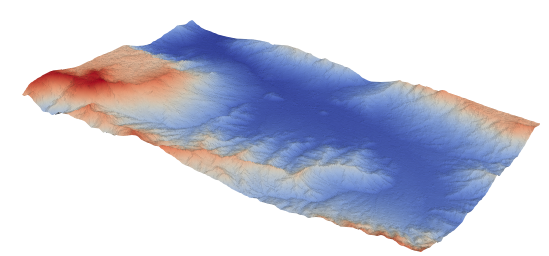
\includegraphics[width=0.90\textwidth]{IMAGES/valle.png}\label{fig:medellin}}
	\caption{\small Overall view of the dominant surface topography in the Aburrá valley region.}
	\label{fig:medallo}
\end{figure}


%
\subsection*{Computational model}
%
Topographic effects for this scenario have been addressed before using large scale computing, see \cite{restrepo2016effects}. However here we will concentrate not in the complete prediction of the ground motions considering mechanical and geometrical effects, but only in the determination of the modifications experienced by the incident motions due to the global surface topography. The analysis is conducted with a frequency domain implementation of the boundary element method \citep{banerjeeboundary} with an explicit consideration of the Sommerfeld radiation condition at infinity. A typical mesh is shown in \cref{fig: bem_mesh} while the model parameters are presented in \cref{tab:bem_params}. We found the response under vertically incident $SH$ and $SV$ waves.


\begin{figure}[H]
	\center
    \subfigure{\includegraphics[width=7cm]{IMAGES/bem_mesh.pdf}}
	\caption{\small Typical boundary element mesh of a cross-section in the Aburra valley region.}
 \label{fig:bem_mesh}
\end{figure}


\begin{table}[H]
\begin{center}
    \begin{tabular} { | c | c | c | c | p{10cm} |}
    \hline
     $Polarization$ & $\beta$ & $\f_{max}$ & $N$ \\ \hline
     %
    $SV$ & $1.0$ & $4.0 Hz$ & $10$  \\ \hline
    %
    $SV$ & $1.0$ & $4.0 Hz$ & $10$  \\ \hline
   \end{tabular}
\end{center}
\caption {Model parameters used in the boundary element models.} \label{tab:bem_params} 
\end{table}


As input motions we used synthetic seismograms using a seed and a target response spectra. As seeds we selected recordings from the Hector Mine and South Napa earthquakes in at last two stations. \Cref{fig:semilla} display the acceleration time signal and response spectra for the horizontal components at the Manchester station. The seeds were modified to produce maximum response spectral amplitudes in a period range between $0.5 s$ and $5.0 s$. \Cref{fig:sinteticos} shows the modified signal and its corresponding response spectra. The spectra shown by the dashed line corresponds to the target response spectra.


\begin{figure}[H]
	\centering
   \subfigure{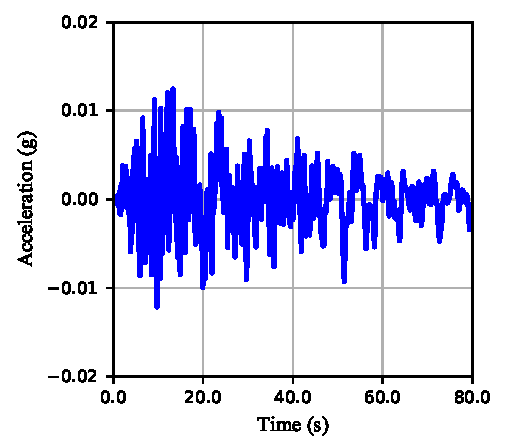
\includegraphics[width=0.45\textwidth]{IMAGES/ManchesterEW.pdf}}
    \subfigure{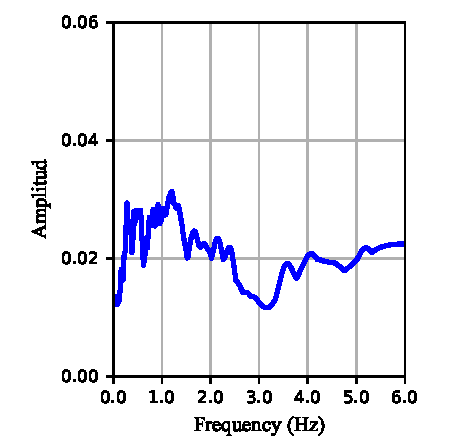
\includegraphics[width=0.45\textwidth]{IMAGES/Manchester_Sa_EW.pdf}}\\
    \subfigure{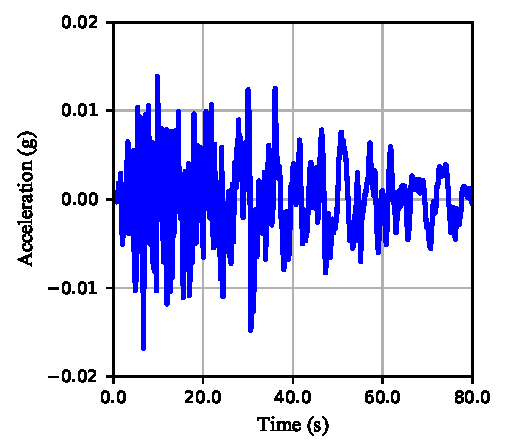
\includegraphics[width=0.45\textwidth]{IMAGES/ManchesterNS.pdf}}
    \subfigure{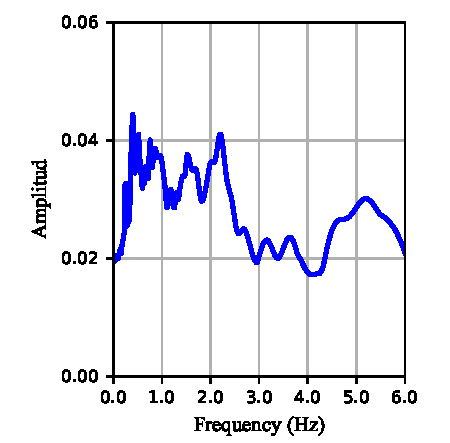
\includegraphics[width=0.45\textwidth]{IMAGES/Manchester_Sa_NS.pdf}}
\caption{Señales de tiempo y Espectros de respuesta de registros en Sismo de Hector Mine, estación Manchester.}
 \label{fig:semilla}
\end{figure}

\begin{figure}[H]
	\centering
   \subfigure{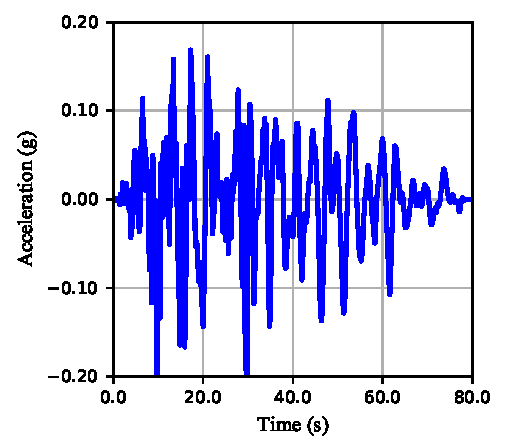
\includegraphics[width=0.45\textwidth]{IMAGES/Manchester_Time_Match_EW.pdf}}
    \subfigure{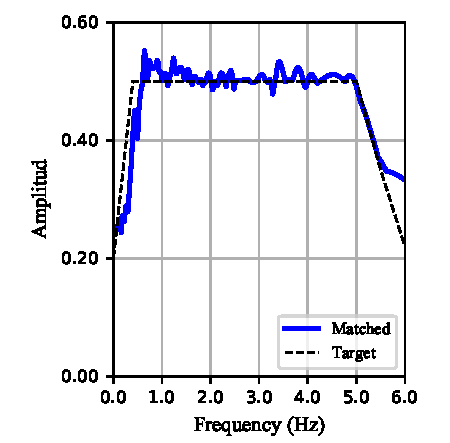
\includegraphics[width=0.45\textwidth]{IMAGES/Manchester_Sa_Match_EW.pdf}}\\
    \subfigure{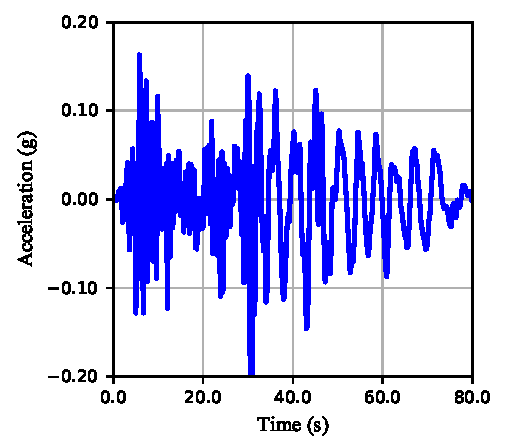
\includegraphics[width=0.45\textwidth]{IMAGES/Manchester_Time_Match_NS.pdf}}
    \subfigure{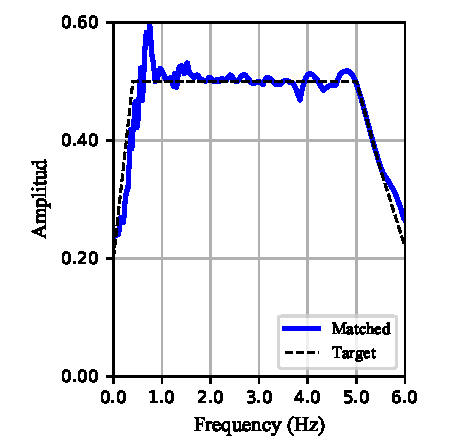
\includegraphics[width=0.45\textwidth]{IMAGES/Manchester_Sa_Match_NS.pdf}}
\caption{Señales sintéticas ajustadas a espectro objetivo.}
 \label{fig:sinteticos}
\end{figure}



\subsection*{Dynamic response}
\Cref{fig:secciones1} shows the two cross sections analyzed in this work. In general, both sections are representative of the topographic layout prevailing in the region with soft slopes or an almost flat configuration in the center and steeper slopes in the west and east margins. The east margin is particularly important as it continues its extension along a second flat region (not shown in the figure) with an increasing growth in population. Each plot includes  a shaded rectangle showing the cross section to be analyzed and its corresponding topographic profile (with distorted vertical scale) with the different response points. In both cross sections points labeled 1 correspond to a localized topographic feature in the form of a V-shaped hill, while points labeled 6 correspond to the flat upper region in each case clearly resembling perfect half-space conditions. The first cross section is conformed by a localized hill in the eastern part of the valley known as Cerro Volador and steep slopes towards the western part of the section. Similarly, the second section includes a localized hill were topographic effects are clearly expected, and relatively easy to predict even using results from idealized theoretical models. This cross section is complemented by slopes ranging between $10\%$ to $15\%$ towards the eastern margin finishing in a flat configuration in the region known as San Nicolas valley. For both cross sections we conducted analysis under SV and SH vertically incident plane waves.

\begin{figure}[H]
	\centering
   \subfigure{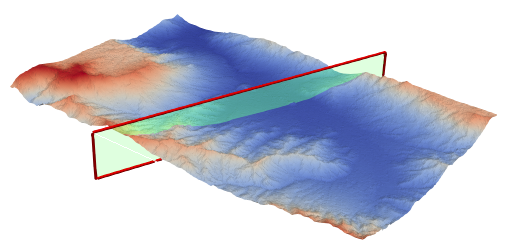
\includegraphics[width=0.45\textwidth]{IMAGES/Nutibara.png}\label{fig:nuti}}
	\subfigure{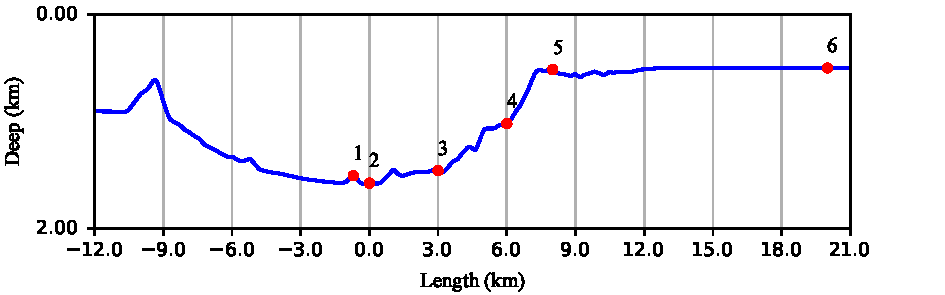
\includegraphics[width=0.50\textwidth]{IMAGES/PerfilNutibara.pdf}}\\
	\subfigure{\includegraphics[width=0.45\textwidth]{IMAGES/volador.png}\label{fig:vola}}
		\subfigure{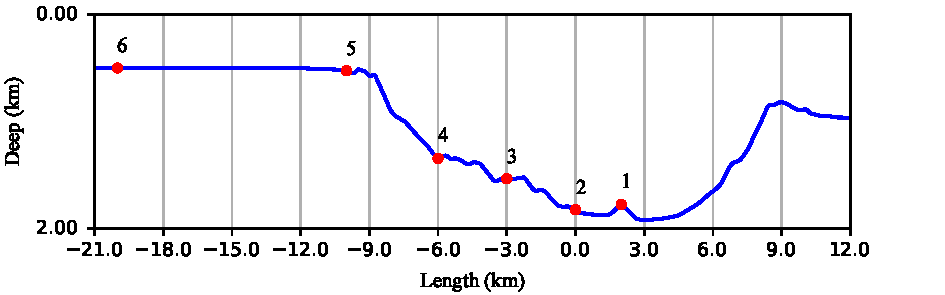
\includegraphics[width=0.50\textwidth]{IMAGES/PerfilVolador.pdf}}
	\caption{\small Overall view of the dominant surface topography in the Aburra valley region. The shaded rectangles correspond to the two east-west cross sections analyzed in this work. Both sections contain a localized topographic feature in the form of an isolated hill in the center of the valley and a stronger coupled topography towards the east and west margins. In both cases the slopped parts of the topographic scenario are highly populated with a large density of reinforced concrete buildings with varying quality levels.}
	\label{fig:secciones1}
\end{figure}


\Cref{fig:SaptosNutEWSV_fisica} to \cref{fig:SaptosVolEWSH_fisica} show the spectral response for both cross sections along the 6 receiver points under vertically incident $SV$ and $SH$ waves for the east-west component of the Manchester record. The spectral amplitudes labeled as 1D in the different plots corresponds to the target response spectra and motion amplification or deamplification due to topographic effects is judged based upon the response relative to this 1D model.

We extract the following main observations from the dynamic response:

\begin{itemize}
\item The response at point 1, corresponding to the localized topography in both cross sections and marked by important amplification over all the period band, appears to be consistent with predictions from theoretical models.
\item The response at point 2, corresponding to the toe of the localized topography in both cross sections and marked by motion deamplification over all the period band appears to be consistent with predictions from theoretical models.
\item The response at points 2, 3 and 4 along the sloped part of the region and conformed by localized topographies of various characteristic dimensions shows spatial variations in motion.
\item The response at point 5,  corresponding to the the upper part of the region near the crest of the canyon shows strong amplification.
\item The response at point 6,  is consistent with half-space conditions.
\end{itemize}

From the geometric point of view present in both cross sections we can identify the following general typologies: (i) localized or isolated topographies with small characteristic dimension expected to produce changes in the high frequency regime (ii) clusters of concave and convex shapes with strong interaction expected to produce complex interference patterns (iii) large scale or regional topography expected to influence the low frequency regime and (iv) localized zones near sharp changes in slope. In the remaining of this work we will use the terms isolated and coupled when referring to cases (i) and (iii) to (iv) respectively. As pointed out previously most of the theoretical works have been devoted to the study of isolated topographies while the coupled general case has been studied exclusively by numerical models. The complexity in the scenario and the variability in the numerical results clearly demonstrate the challenge involved in the development of simplified analysis procedures for topographic effects. This research aims at developing physical understanding of the scattering of waves in such complex geometric scenarios with the goal of identifying controlling parameters. Although the variability of the results suggest that in order to predict the nature of the ground motions, even at the practicing level, the analysis necessarily requires the use of numerical simulation, here we intend to provide guidelines that can be used for the construction of the proper numerical model at specific conditions. 

\begin{figure}[H]
	\center
    \subfigure{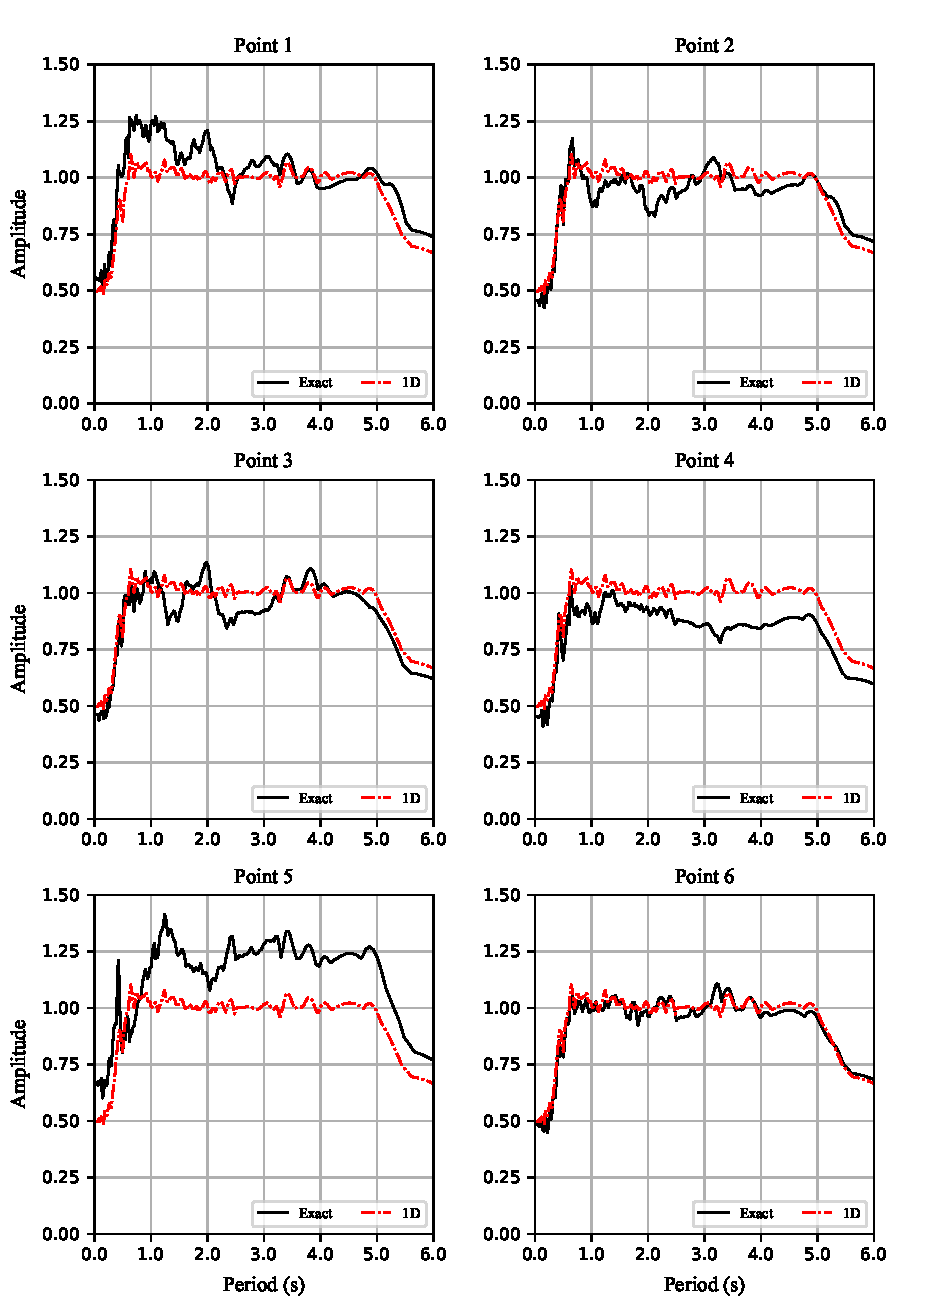
\includegraphics[scale=0.7]{IMAGES/Spectral_Nutibara_Manchester_EW_SV_fisica.pdf}}
	\caption{\small Acceleration response spectra along the 6 receiver points in the cerro Nutibara cross section under vertically incident SV waves. The trace marked as target corresponds to the response spectra under perfect half-space conditions}
 \label{fig:SaptosNutEWSV_fisica}
\end{figure}

\begin{figure}[H]
	\center
    \subfigure{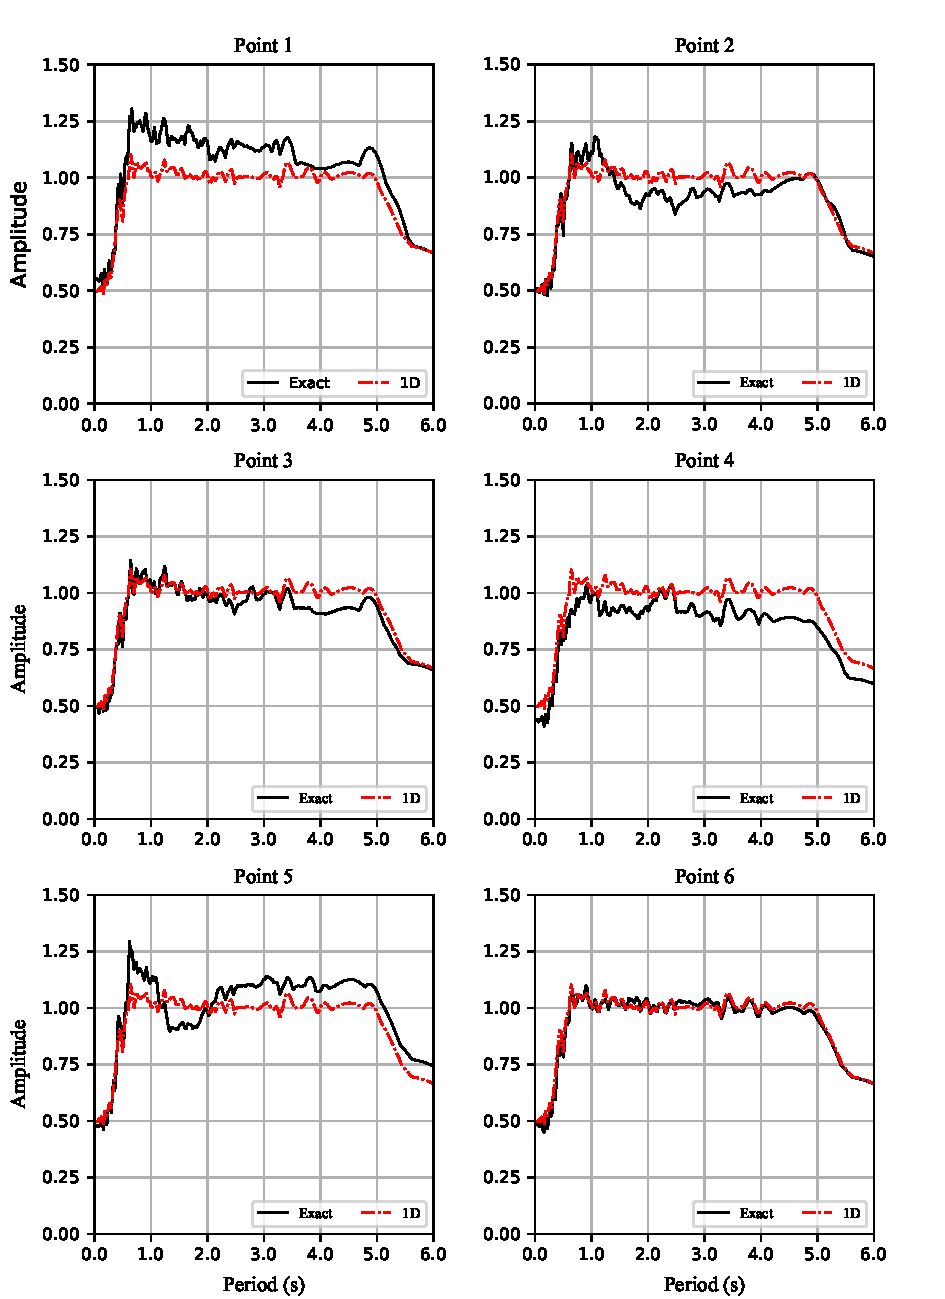
\includegraphics[scale=0.7]{IMAGES/Spectral_Nutibara_Manchester_EW_SH_fisica.pdf}}
	\caption{\small Acceleration response spectra along the 6 receiver points in the cerro Nutibara cross section under vertically incident SH waves.The trace marked as target corresponds to the response spectra under perfect half-space conditions}
 \label{fig:SaptosNutEWSH_fisica}
\end{figure}

\begin{figure}[H]
	\center
    \subfigure{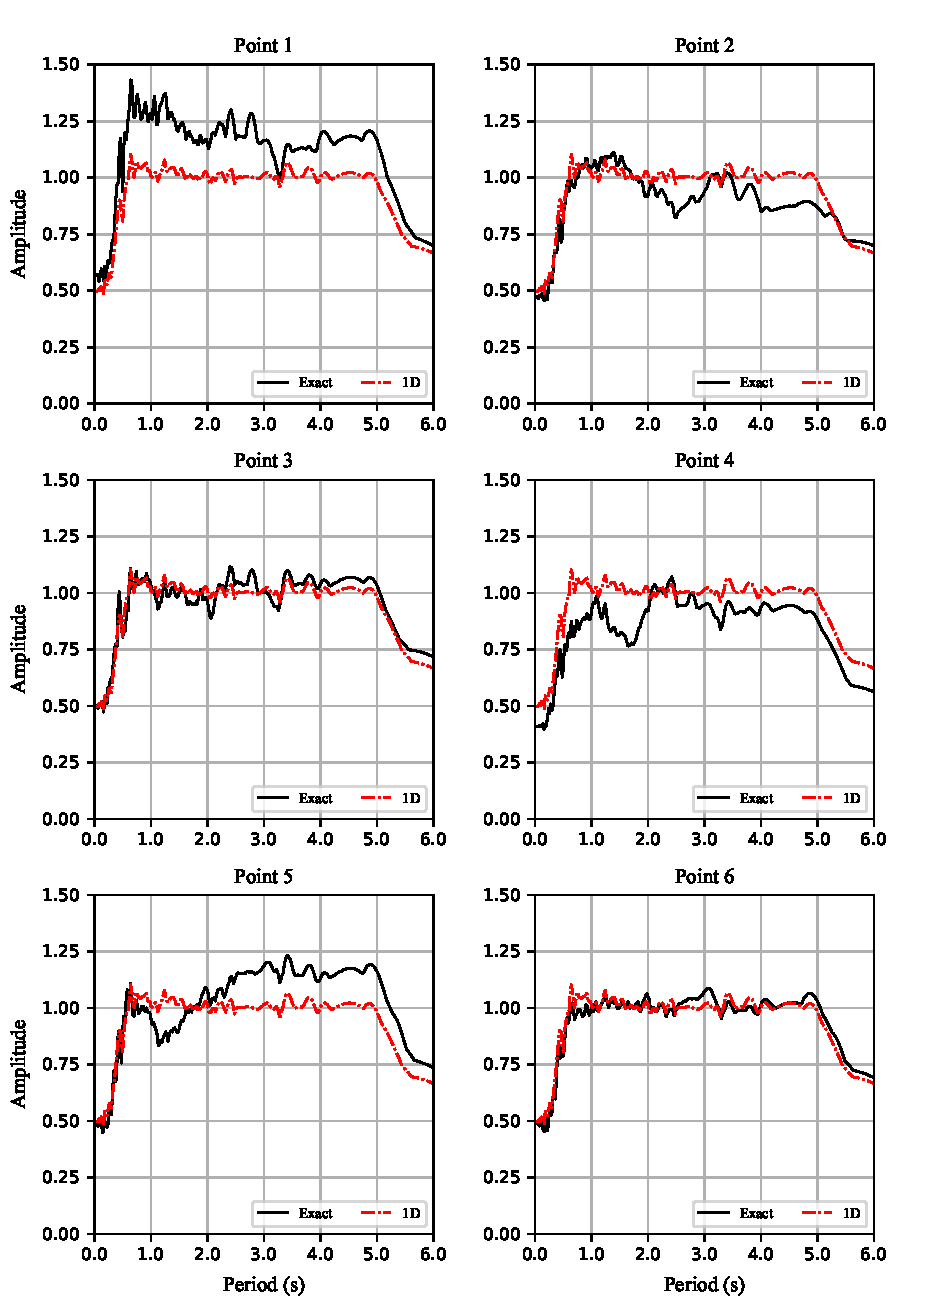
\includegraphics[scale=0.7]{IMAGES/Spectral_Volador_Manchester_EW_SV_fisica.pdf}}
	\caption{\small Acceleration response spectra along the 6 receiver points in the cerro Volador cross section under vertically incident SV waves. The trace marked as target corresponds to the response spectra under perfect half-space conditions}
 \label{fig:SaptosVolEWSV_fisica}
\end{figure}

\begin{figure}[H]
	\center
    \subfigure{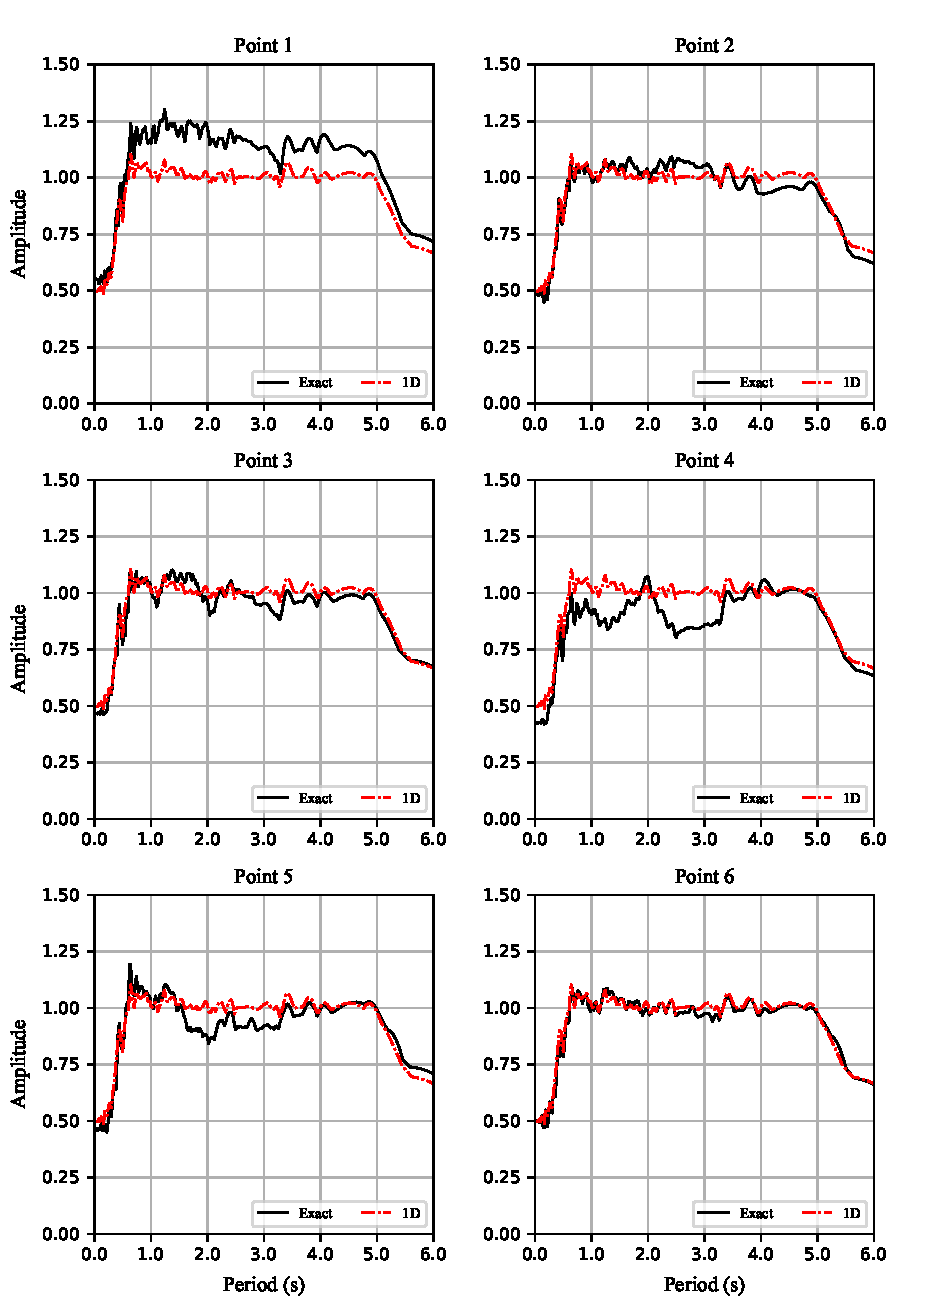
\includegraphics[scale=0.7]{IMAGES/Spectral_Volador_Manchester_EW_SH_fisica.pdf}}
	\caption{\small Acceleration response spectra along the 6 receiver points in the cerro Volador cross section under vertically incident SH waves. The trace marked as target corresponds to the response spectra under perfect half-space conditions.}
 \label{fig:SaptosVolEWSH_fisica}
\end{figure}






%\end{itemize}
\subsection*{Conclusions}
We determined the dynamic response of two cross sections of the Aburrá valley region in Medellín, Colombia under vertically incident horizontally and vertically polarized shear waves. This geometric scenario is highly interesting for the study of topographic effects since it is realistic and at the same time offers several conditions of geometric typology.

The analysis was conducted with a frequency domain based boundary element code thus explicitly accounting for radiation boundary conditions at infinity. The resulting transfer functions were convoluted with an acceleration time history synthetically produced out of a seed earthquake and scaled to match a target response spectra with near constant amplitude in the period range between $0.5 s$ and $5.0 S$. The resulting acceleration time-histories were later used in the computation of acceleration response spectra at several observation points. The spectral amplitude reveal strong spatial variations in motion due to the topographic effect. As expected, the motion at local isolated topographies is consistent with theoretical observations. On the other hand, the response at two specific locations is of particular interest. First, at receivers located over the steep slopes surrounding the region the topographic effect appears to be rather moderate, probably due to the combination of constructing and destructing interference among the local sites. Second, the observation point located near the upper corner of the region exhibits strong amplification although it is located in a flat zone.




%%%%%%%%%%%%%%%%%%%%%%%%%%%%%%%%%%%%%%%%%%%%%%%%%%%%%%%%%%%%%%%%%%%%%%%
%%%% %%%%%%%%%%%%%%%%%%%%%%%%D I F R A C C I O N%%%%%%%%%%%%%%%%%%%%%%%%%%%%%%%
%%%%%%%%%%%%%%%%%%%%%%%%%%%%%%%%%%%%%%%%%%%%%%%%%%%%%%%%%%%%%%%%%%%%%%%

\newpage

\section{Superposition Based Diffraction}
\phantomsection
\addcontentsline{toc}{section}{Superposition based diffraction}

In this section we introduce our basic analysis method aimed at a rational study of the geometric aggravation introduced by surface topography. As implicitly suggested, since the early beginnings of the study of topographic effects by authors like \cite{ashford1997topographic}, \cite{geli1988effect}, \cite{Trifunac1973}, \cite{sanchez-sesma91}, \cite{sanchez1979ground} just to mention a few, here we focus in the analysis of an infinite wedge, where it is assumed that an arbitrary surface topography can be approximated by a series of neighborhood wedges. A similar idea was also suggested by \cite{mohammadi2017topography} although these authors used mainly numerical simulations. Here we restrict ourselves to scalar horizontally polarized problems which admit analytic treatments. In fact, since the solution for an infinite wedge can be separated into a geometrical and a diffracted field we show that the solution for a superposition of wedges can be built after patiently adding sources of diffraction. In consequence we have termed the resulting method of analysis the superposition based diffraction technique. Although the method is tedious if one intents to apply it to a very complex geometry it is a strong conceptual tool useful in the interpretation of results from a numerical analysis even in the case of more complex in-plan vector wave propagation problems.



\subsection*{Alternative representation of the total response}
\addcontentsline{toc}{subsection}{Alternative representation of the total response}

The basis of the current superposition based diffraction (SBD) approach is the linear character of the problem. This allows the total solution to be written in terms of the addition of different and arbitrary superpositions. For instance, one such partition corresponds to the usual earthquake engineering definition of free-field motion allowing to express the total field like

\begin{equation}
\label{free field}
{u^T}={u^0_A}+{u^S_A}
\end{equation}

and where $u^0_A\equiv u^{IN}+u^R_A$ is the free-field with $u^S_A$ being the scattered motion. In the above $u^{IN}$ and ${u^R_A}$  represent the incident motion and the field reflected in an equivalent perfect half-space. By reasons that will become apparent later, we refer to the free-field term $u^0_A$ like the artificial incoming motion.


An alternative partition of the total response, introduced in \cite{gomez2013analysis}, and constituting the basis of our method is now explained with reference to \cref{fig:part} which schematically describes a scattering problem where the domain $\Omega \cup \Omega^+$ (left) has been partitioned into the scatterer $\Omega$ (bottom) and its supporting half-space $\Omega^+$ (top) respectively.

\begin{figure}[H]
\centering
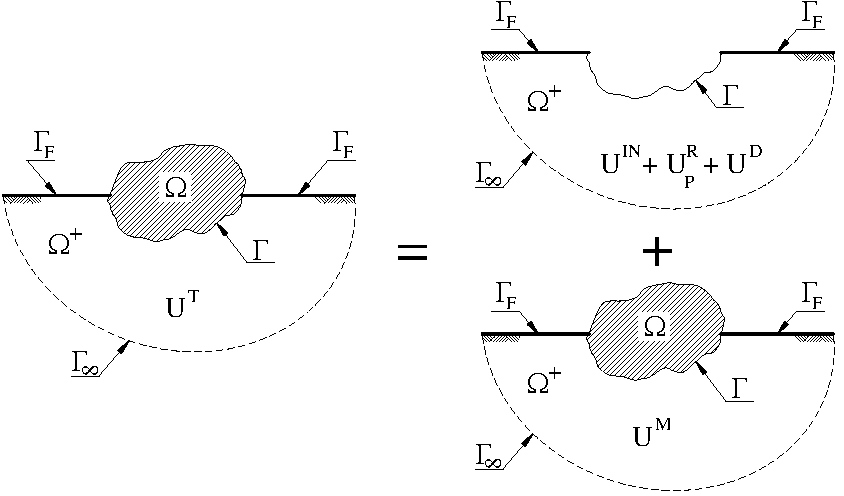
\includegraphics[width=10cm]{IMAGES/mec.pdf}
\caption{Partition of the the total domain into sub-domains. The total problem is divided into a generalized supporting half-space of domain $\Omega^+$ and a scatterer of domain $\Omega$. The solution for the generalized half-space is constructed by the addition of an optical field $u^{IN}+u_P^R$ plus its diffractions $u^D$ over the irregularity $\Gamma$.
\label{fig:part}}
\end{figure}

Based upon the above partition of the total problem into sub-domains we can subsequently write for the total field as:

\begin{equation}
\label{total field 1}
{u^T}={u^{IN}}+{u^R_P}+{u^D}+{u^M}
\end{equation}

where the first three terms correspond respectively to the incident field; its reflections over the free-surface $\Gamma + \Gamma_F$ (notice that $\Gamma$ becomes exposed after having removed the scatterer from the half-space); and the diffracted field. This last term in the solution is required in order to restore continuity of the field since the contribution from ${u^{IN}}+{u^R_P}$ is incomplete due to the geometric singularitues existing along $\Gamma$. If we identify the first two terms in \cref{total field 1} like the optical field $u^0_P$ we can re-write the total solution like;

\begin{equation}
\label{total field 2}
{u^T}={u^0_P}+{u^D}+{u^M}.
\end{equation}

Clearly, in \cref{total field 2} $u^M$ is an additional field introduced by the scatterer $\Omega$. The name {\it artificial incoming motion}, previously coined to the engineering free-field definition $u^0_A$ is now evident since such definition, according to \cref{free field}, leads to the concept of the scattered field which has mainly a mathematical meaning. If we now consider the term ${u^D}+{u^M}$ like an alternative scattered motion or relative displacement $u^S_P$ corresponding to a difference between the total solution and the optical field, then \cref{total field 2} can be written like;

\begin{equation}
\label{P free field}
{u^T}={u^0_P}+{u^S_P}
\end{equation}

which is analogous to the classical partition given by \cref{free field} in terms of the free-field and the mathematical scattered motion. In fact, this alternative definition of the scattered field and the commonly used classical definition are easily shown to be connected by;

\begin{equation}
\label{diffraction to scattered}
{u^S}={u^R_P}-{u^R_A}+{u^S_P}.
\end{equation}

In problems involving only a topographic irregularity where $u^M=0$ and ${u^S_P}={u^D}$ the total field can be written like;

\begin{equation}
\label{diffracted field}
{u^T}={u^0_P}+{u^D}.
\end{equation}

Since in the case of horizontally polarized motions the optical field (OF) (or physically based incoming motion $u^0_P$), can be obtained analytically, the construction of the total solution becomes feasible as long as we find a way to compute the contribution from the diffracted field. This term can be obtained following the work in \cite{jaramillo2013analytic} in terms of the diffracted field for a generalized infinite wedge and where the topographic irregularity is represented as a superposition of wedges of different inclinations and perceiving the incident wave at different angles.

Although the representation of the total filed as given by the standard form of \cref{free field} is suitable for numerical implementations of the problem, the superposition given by \cref{diffracted field} has a stronger physical basis as it facilitates the direct determination of the diffracted field. Our superposition based technique is grounded in this physical approach.

\subsection*{Fundamental solution}
\addcontentsline{toc}{subsection}{Fundamental solution}

In the proposed SBD method the geometry of the topographic irregularity is constructed via superposition of rectilinear segments using as a fundamental entity the simple infinite wedge shown in \cref{fig:fun_wedge}. Any incident wave, plane or cylindrical, impinging against this fundamental wedge has a solution composed of a closed-form geometrical field  and an additional diffracted term $u^D$.

As we will detail later the solution method for an arbitrary surface topography amounts to (i) approximating the geometry by a series of wedges (ii) building the complete optical field and (iii) adding the resulting diffraction terms.

\begin{figure}[H]
\centering
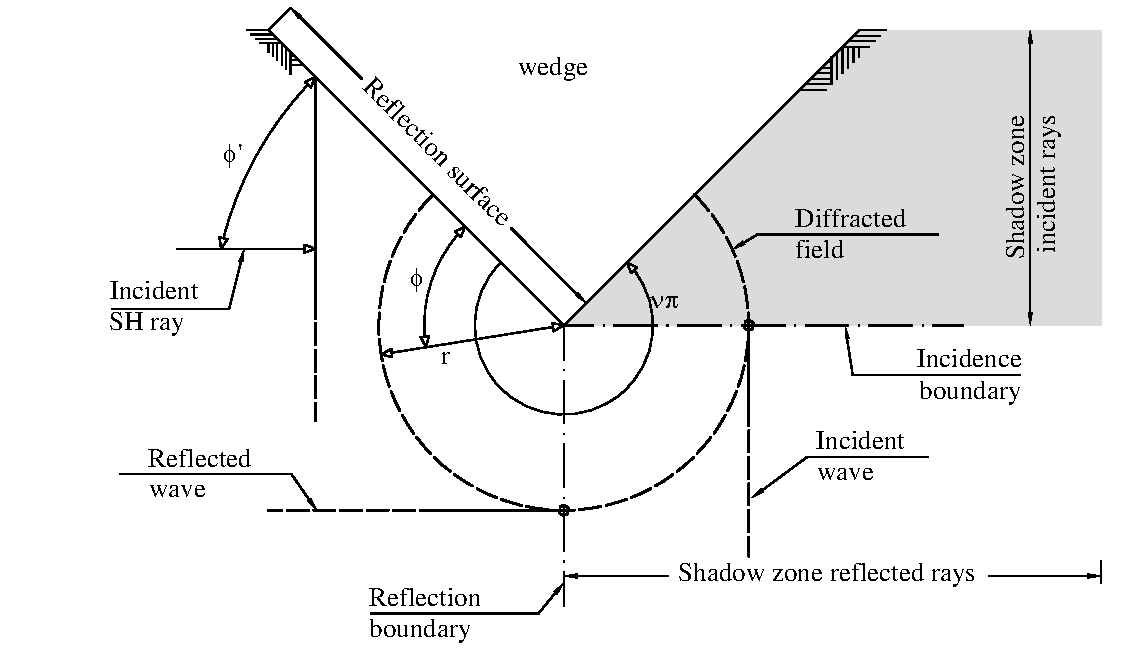
\includegraphics[width=10cm]{IMAGES/figure2.pdf}
\caption{Elementary wedge forming the basis of the SBD approach. The incident ray corresponds to a plane $SH$ front impinging against an infinite wedge. The incident front and its reflection at the traction free surface produces an illuminated zone. Similarly, the region not directly illuminated by the incident and reflected ray corresponds to a shadow zone. The boundary resulting in-between the illuminated and shadow zone corresponds to a region of discontinuity of the incoming field. Continuity is however restored by the cylindrical diffracted wave generated at the singularity point and penetrating into the shadow zone.
\label{fig:fun_wedge}}
%
\end{figure}

The term corresponding to the diffraction field generated by the interaction of the plane (or cylindrical) incident wave with the corner singularity in the wedge is given in \cref{diffraction}. 

\begin{align} \label{diffraction}
u^{D}\left(\phi,r\right)&=A\frac{-e^{\left(-\hat{i}\left(kr+\pi/4\right)\right)}}{2\nu\sqrt{2\pi}\sqrt{kr}}\left[\cot\left(\frac{\pi+\left(\phi-\phi'\right)}{2\nu}\right)F\left(kLa^{+}\left(\phi-\phi'\right)\right)\right.\nonumber\\
&\left.+\cot\left(\frac{\pi-\left(\phi-\phi'\right)}{2\nu}\right)F\left(kLa^{-}\left(\phi-\phi'\right)\right)\right.\nonumber\\
&\left.+\cot\left(\frac{\pi+\left(\phi+\phi'\right)}{2\nu}\right)F\left(kLa^{+}\left(\phi+\phi'\right)\right)\right.\nonumber\\
&\left.+\cot\left(\frac{\pi-\left(\phi+\phi'\right)}{2\nu}\right)F\left(kLa^{-}\left(\phi+\phi'\right)\right) \right]
\end{align}



This solution was proposed by \cite{[1974]KoyPat} in the context of propagation of electromagnetic waves after using the well established geometrical theory of diffraction (GTD), originally proposed by \cite{[1962]Kell} and particularized to the case of horizontally polarized shear $SH$ waves incident against surface topographies by \cite{jaramillo2013analytic}. In \cref{diffraction} $r=$radial coordinate of the field point measured from the vertex of the wedge, $\phi=$ angular coordinate measured with respect to the reflection boundary, $\phi'=$incidence angle measured with respect to the reflection boundary, $\nu\pi=$wedge angle (with $\nu$ being a factor between $0.0$ and $2.0$), $r'=$radius of the incident cylindrical wave (for the diffraction of a cylindrical front), $k=$wave number and $\beta=$velocity of wave propagation.  The remaining terms appearing in \cref{diffraction} are defined as follows;
%
%
\begin{align*}
&F\left(X\right)=2\hat{i}\sqrt{X}e^{\hat{i}X}
\int_{\sqrt{X}}^\infty e^{-\hat{i}\tau^2}\mathrm{d}\tau\\
&L=r\qquad\qquad\text{for incident plane waves}\\
&L=\frac{rr'}{r+r'}\qquad\text{for incident cylindrical waves}\\
&a^{\pm}\left(\theta\right)=2\cos ^{2}\left(\frac{2\nu\pi N^\pm -\theta}{2}\right)\\
&N^+ =
  \begin{cases}
   0 & \text{if } \theta \leq \nu\pi -\pi \\
   1       & \text{if } \theta > \nu\pi -\pi
  \end{cases},\quad N^-=\begin{cases}
  -1 & \text{if } \theta < \pi -\nu\pi \\
   0 & \text{if } \pi -\nu\pi\leq \theta \leq \pi +\nu\pi \\
   1 & \text{if } \theta > \pi +\nu\pi
  \end{cases}
\end{align*}



\subsection*{Superposition of diffracted waves}
\phantomsection
\addcontentsline{toc}{subsection}{Superposition of diffracted waves}

The algorithm to construct the solution is summarized next with reference to the schematic simple $V$-shaped canyon shown in \cref{fig:vshapedcanyon2}. First, the surface geometry has to be approximated by overlapping infinite wedges. Notice that each wedge contributes with 2 surfaces of reflection and 1 source of diffraction, while for each pair of superimposed wedges there is an additional (third) source of diffraction. The second step involves the identification of zones illuminated by the incident and reflected waves and a partition of the domain according to the number of rays existing in these different zones. An additional third step now requires the identification of boundaries between illuminated and shadow zones corresponding to regions of discontinuity of the optical field that must be filled out by the diffraction field. These regions generate a second subdomain partition. The fourth step requires the computation of the optical and diffracted fields in each one of their sudomains of existence: in this last step the interaction between sources of diffraction must also be considered. These corresponds to cylindrical waves incident against the corner singularity. The inclusion of each new source amounts to an application of the expression given in \cref{diffraction} with the values of the parameters properly adjusted to the particular case and with each one of them contributing with an additional term to the series solution. The details involved in the partition of the total domain into sub-domains are elaborated next.
%
\begin{figure}[H]
\centering
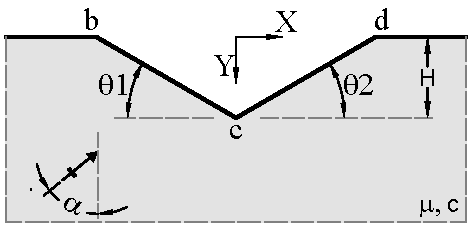
\includegraphics[width=10cm]{IMAGES/vshaped1.pdf}
\caption{Symmetrical $V$-shaped canyon representable by 3 wedges with appex at points $b$, $c$ and $d$ respectively. Each wedge contributes with a source of diffraction
 acting upon the main plane incident front (first order diffracttion) or upon the cylndrical waves generated at adjacent wedges (higher order diffraction).
\label{fig:vshapedcanyon2}}
\end{figure}
%
\subsubsection*{Step I: representation of the surface geometry}
\addcontentsline{toc}{subsubsection}{Step I: representation of the surface geometry}

In the first analysis step the surface topography is represented by a superposition of several wedges of the type described in \cref{fig:fun_wedge}. A wedge is defined by the angular parameter $\nu \pi$ and by the angle of incidence of the plane wave $\phi'$ as given in \cref{diffraction}. Here we denote the $i-th$ wedge by $C_i$. Each newly introduced $C_i$-wedge contributes with two traction free boundaries and a diffractor (or source of diffraction) denoted by $D_i$. The traction free surfaces are reflectors and therefore regarded as continuous sources. The wedges required to represent the $V$-shaped canyon are shown in the left part of \cref{fig:wedges} and have been denoted like $C_1$, $C_2$ and $C_3$ respectively. The arrows in the figure show the source of diffraction and the two reflection surfaces contributed by each wedge.

\begin{figure}[H]
\centering
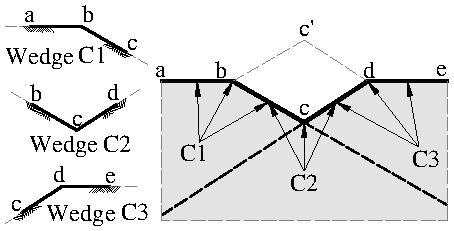
\includegraphics[width=10cm]{IMAGES/vshapedw.pdf}
\caption{Representation of the $V$-shaped canyon through the superposition of infinite wedges. Each wedge contributes with a discrete source of diffraction and two continuous sources of reflected rays represented by the free boundaries. Each point singularity introduces a boundary of discontinuity in the optical field. Full continuity is restored by the  diffracted waves emanated by the tips.
\label{fig:wedges}}
\end{figure}

\subsubsection*{Step II: partition of the domain}
\addcontentsline{toc}{subsubsection}{Step II: partition of the domain}

The computational domain is now partitioned into convenient sub-domains according to the regions of existence of the fields contributed by the different sources. Here we consider the regions of existence of different waves in terms of rays. In a first step we consider the main incident wave and its reflections at the free boundaries. We will refer to this partition as the free-field-partition. Notice that the definition of this subdomain is clearly dependent upon the angle of incidence.

To clarify we show in \cref{fig:zones} the free-field-partition for an asymmetric $V$-shaped canyon subjected to a vertically incident $SH$ wave. The first region is determined by the incident wave (denoted in the figure by the ray $R1$). In this problem the incident ray exists throughout the complete domain. The second region is the reflection zone defined by the existence of the downward-vertically-propagating waves (denoted in the figure by the rays $R2$). These appear as a result of the reflection at the horizontal free boundaries of the half-space. The last and final sub-domain is the region enclosed by the diagonal lines defining the region of existence of rays reflected at the inclined free faces of the canyon (denoted in \cref{fig:zones} by the rays $R3$ and $R4$).

In the final partition step regarding the continuous sources, the above three partitions are added (or superimposed) showing the contribution from the incoming field in terms of rays at all the different points inside the problem domain. After considering interceptions of regions a total of 6 different zones are identified: these are enclosed by circles in \cref{fig:zones}. It should be noticed that only the rays originated at the inclined boundaries must be phase-corrected considering the used system of reference. Also, notice that the rays $R3$ and $R4$ are reflected downward as long as the angles $\theta_1 \equiv \theta_2 \leq \pi/4$. In a more general case, the rays reflected by the inclined free surfaces of the canyon may experience subsequent reflections at the horizontal part of the half-space leading to a different free-field-partition.

\begin{figure}[H]
\centering
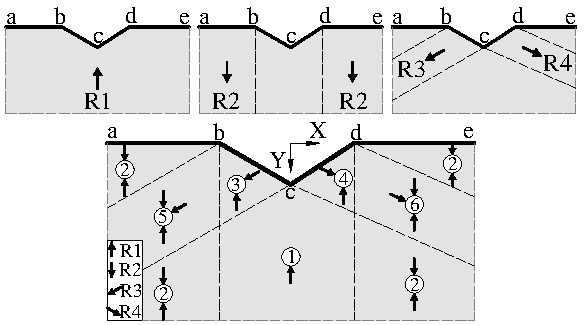
\includegraphics[width=10cm]{IMAGES/00_Propuesta_1.pdf}
\caption{Partition of the domain to compute the free field. Regions of existence of different rays are identified. $R1$ corresponds to the zone illuminated by the main incident front; $R2$ is the region of existence of reflection over the horizontal free surface; and $R3$ and $R4$ correspond to the reflections over the inclined surfaces. Since multiple rays may exist over a given region the total number of rays is described by a number enclosed by circles (bottom part of the figure).}
\label{fig:zones}
\end{figure}

The second superposition step consists in the consideration of the diffracted field. For this purpose we perform a second partition of the computational domain, analogous to the one used for the free field, but now dictated by regions of existence of diffraction terms. As already pointed out each wedge contributes with cylindrical diffracetd waves emanated from a source at its apex producing a sub-domain related to the region of existence of the originating wedge. This partition is described in \cref{fig:zones of diffraction} and in what follows we refer to such specific consideration of the domain as the diffracted-field-partition.

\begin{figure}[H]
\centering
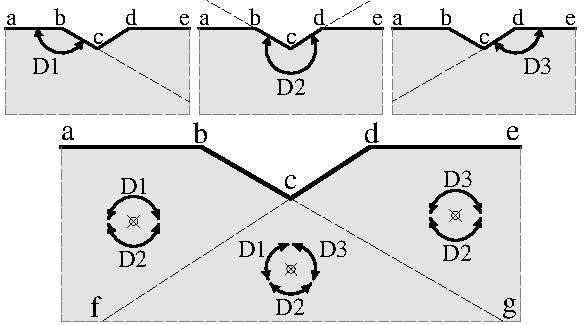
\includegraphics[width=10cm]{IMAGES/00_Propuesta_2.pdf}
\caption{Partition of the domain to compute the diffracted field. Each wedge contributes with a source of diffraction producing waves over a given part of the domain (top). Zones where the contribution from several wedges overlap are indicated by the curved rays.}
\label{fig:zones of diffraction}
\end{figure}


The corresponding diffracted rays have been labeled $D1$, $D2$ and $D3$. For instance, the diffracted rays $D2$ exist throughout the complete domain, while the rays labeled $D1$ and $D3$ exist only inside the domains delimited by the lines $a-b-c-g$ and $e-d-c-f$ respectively. The final superposition of the 3 sub-domains is represented by crossed circles with their related diffracted rays (see \cref{fig:zones of diffraction}).

\subsubsection*{Step III: higher order diffraction contribution}
\addcontentsline{toc}{subsubsection}{Step III: higher order diffraction contribution}

In the above superposition process, the geometric singularity associated to each subdomain, may diffract either the main plane front corresponing to the incoming field or the cylindrical waves originated at adjacent wedges. Hereafter we refer to the first effect like primary diffraction while subsequent diffraction events are refered to like higher order diffraction. Both, the first and higher order diffraction contribution represent terms in the series solution. However, since each diffracted wave has an amplitude smaller than its originating source, only a few terms need to be retained in the series. Let us consider the diffraction field generated by the central wedge with apex at point $c$ in \cref{fig:zones of diffraction}. The diffracted field generated by this source can be written like;

\begin{multline}
u^D=u^D_c+u^D_{b-c}+u^D_{d-c}+u^D_{c-b-c}+u^D_{c-d-c}+u^D_{b-....-c}\\
+u^D_{c-....-c}+u^D_{d-....-c}. 
\label{diffraction of the diffraction}
\end{multline}

In \cref{diffraction of the diffraction} the first subscript in each term indicates the originating source. Accordingly the term $u^D_c$ corresponds to a diffracted wave with source at c while the last subscript indicates the diffractor. Also the number of subscripts in each term indicates the order of the diffraction. For instance, the term $u^D_c$ describes the diffraction of the main front at point $c$; the term $u^D_{b-c}$ is the second order diffraction (indicated by two subscripts) introduced by the diffractor $c$ (indicated by the last subscript) of the cylindrical wave with source at $b$ (indicated by the first subscript). Similarly, the term $u^D_{c-b-c}$ is the third order diffraction produced by the diffractor $c$ which diffracts a cylindrical wave with source at $c$, diffracted at $b$ and diffracted again at $c$.

\Cref{fig:highorder} shows an schematic representation of snapshots of the different diffracted fronts generated by the wedges of the $V$-shaped canyon. At the time instant $t2$ the cylindrical front identified at the lower appex corresponds to the first-order diffraction. Similarly, at time $t3$ there are two sets of cylindrical fronts generated at the upper wedges. The large front is once again the main or first-order diffraction, while the small ones correspond to second-order diffraction experienced by the cylindrical wave generated at $t2$. These fronts subsequently experience third-order diffraction at $t5$.

\begin{figure}[H]
\centering
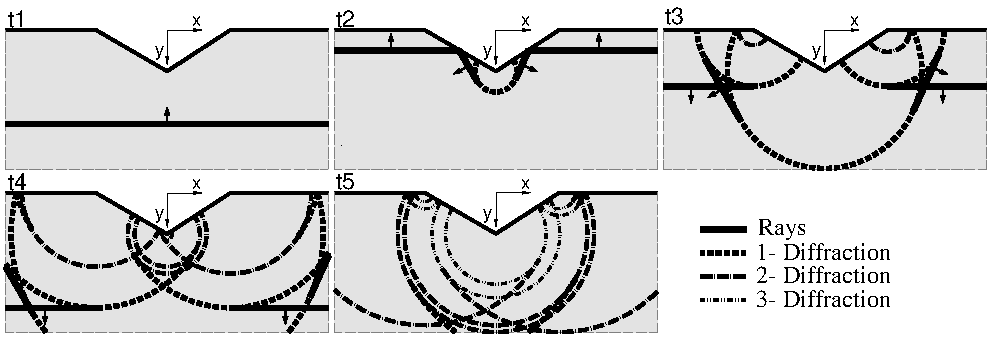
\includegraphics[width=12cm]{IMAGES/00_Propuesta_3.pdf}
\caption{Schematic snapshots showing the main front, the reflected field and cylindrical diffracetd waves up to $3$-rd order. At $t2$ the incident front is first-order diffracted at point $c$. This same front first-order diffracts at points $b$ and $d$ at $t3$, while the first formed cylindrical front experiences second-order diffraction at these points. Third first third order diffraction event is identified at $t5$ at point $c$.}
\label{fig:highorder}
\end{figure}

The solution process now reduces to the addition of the free and diffracted fields as imposed by their domains of existence (previously defined like free-field-partition and diffracted-field-partition).

The diffracted field is obtained after successive applications of the fundamental solution given in \cref{diffraction} with arguments corresponding to a plane or to a cylindrical wave according to each case. In order to clarify this last step, we show in \cref{tab:high order} the arguments for the evaluation of the second order diffraction resulting after the cylindrical wave generated at the source point $c$ interacts with the wedges with vertices at points $b$ and $d$. According to the notation introduced previously these terms are denoted like $u^D_{c-b}$ and $u^D_{c-d}$ respectively.

\begin{table}[H]
\begin{center}
    \begin{tabular}{ | c | c | c | c | c | p{10cm} |}
    \hline
     $Term$ & $\nu \pi$ & $\phi'$ & $r'$ & $Geometry$ \\ \hline
     %
    $u^D_c$ & $\theta_1+\theta_2+\pi$ & $\theta_1+\pi/2$ & $-$ & 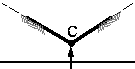
\includegraphics[width=2.5cm]{IMAGES/wc.pdf} \\ \hline
    %
    $u^D_b$ & $\pi-\theta_1$ & $\pi/2$ & $-$ & 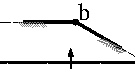
\includegraphics[width=2.5cm]{IMAGES/wb.pdf} \\ \hline
    %   
    $u^D_d$ & $\pi-\theta_2$ & $\pi/2-\theta_2$ & $-$ & 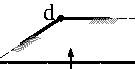
\includegraphics[width=2.5cm]{IMAGES/wd.pdf} \\ \hline
    % 
    $u^D_{c-b}$ & $\pi-\theta_1$ & $\pi-\theta_1$ & $\overline{c-b}$ & 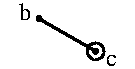
\includegraphics[width=2.5cm]{IMAGES/wcb.pdf} \\ \hline
    %
    $u^D_{c-d}$ & $\pi-\theta_2$ & $0$ & $\overline{c-d}$ & 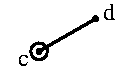
\includegraphics[width=2.5cm]{IMAGES/wcd.pdf} \\ \hline 
   \end{tabular}
\end{center}
\caption {Arguments for the evaluation of the diffraction terms appearing in \cref{diffraction of the diffraction} according to \cref{diffraction}.} \label{tab:high order} 
\end{table}

\subsubsection*{Step IV: Construction of the total solution}
\addcontentsline{toc}{subsubsection}{Step IV: Construction of the total solution}
The complete solution now involves the addition of the field existing within each subdomain. In general we can write;


\begin{multline}
{u^T}=u^{IN}+u^R_P+u^D_c+u^D_a+u^D_b+u^D_{b-c}\\
+u^D_{d-c}+u^D_{c-b-c}+u^D_{c-d-c}+u^D_{c-d-....-c}+... 
\label{total sln}
\end{multline}

although as implied by \cref{total sln}, the solution takes the form of an infinite series where each term with an increasing number of subscripts corresponding to higher order diffraction has a decreasing amplitude. Our solution has the advantage over those found using eigenfunction expansions, that the approach does not require the problem geometry to correspond to a separable system of coordinates and the fact that here each term of the series has a physical meaning associated to the diffraction contributions of various orders. As such, the approximation is conducted on physical grounds rather than on convergence analysis based on mathematical arguments. Moreover, since the truncated terms are related to the diffracted field, which is known to be frequency dependent, the stopping criteria depends on the dimensionless frequency of the particular problem under study.

\subsection*{Validation of the SBD approach}
\addcontentsline{toc}{subsection}{Validation of the SBD approach}

As a verification and validation of the proposed SBD approach we solved the $V$-shaped canyon previously studied by a wave function expansion method in \cite{tsaur2008analytical}. The canyon response was computed for values of the depth-to-width aspect ratio $d/a$ corresponding to $[0.25, 0.50, 0.75, 1.0]$ covering both, shallow and deep canyons. The analyses were conducted for a dimensionless frequency $\eta=2a/\lambda=1.0$ and for unitary values of the wave propagation velocity and mass density.

\Cref{fig:SBD_Tsaur} compares the spatial distribution of the amplitude function over the free surface. The first row compares the solution by \cite{tsaur2008analytical} and the SBD results for 1, 2 and 3 orders of diffraction respectively, while in rows 2, 3 and 4 we show these same results independently. Similarly each column in \cref{fig:SBD_Tsaur} compares the wave function solution with the SBD results for the different values of the aspect ratio. It is observed how, independent of the number of orders of diffraction considered in the SBD solution, the results degrade in the direction of increasing aspect ratio. However, it is evident that 3 orders of diffraction suffice to reach  a solution comparable to the one reported by \cite{tsaur2008analytical} even for the deep canyon ($d/a=1.0$), while 2 orders of diffraction are enough in the case of a shallow valley. If one takes advantage of the symmetry of the domain the solution with 3 orders of diffraction amounts to a total of 8 terms in the SBD series while the same result requires the evaluation of 24 terms if one follows the region matching technique formulated by \cite{tsaur2008analytical}.
%

\subsection*{Response of a $25^\circ$ $V$-shaped canyon}
\addcontentsline{toc}{subsection}{Response of a $25^\circ$ $V$-shaped canyon}

In order to test the accuracy of the SBD technique, we conducted frequency and time domain analysis of the simple $V$-shaped canyon topography using our proposed method and a numerical boundary element (BEM) based algorithm. We first found the response of the system to harmonic plane waves of unit amplitude described in terms of the dimensionless frequency $\eta=H/\lambda$ where $H$ is the canyon height and $\lambda$ the corresponding wavelength of the incident wave. In all our analyses we considered a $25^\circ$ canyon while the depth parameter $H$ was varied according to the dimensionless frequency $\eta$. We obtained the response at values of $\eta$ between $0.0625$ and $15.0$. The frequency domain results were used later in order to find the time domain response using a Fourier transformation approach. For that purpose we used a Ricker pulse defined according to $R(t) = (2\pi\tau-1)e^{-\pi\tau^2}$, where $\tau=f_c(t-t_{ini})$ with $f_c$= central frequency and $t_{ini}$=initial time for the intense phase. In this work we used a pulse with a central frequency $f_c=8.0Hz$ and the initial time was adjusted to generate a time window conveniently fitting the selecetd computational domain.

\Cref{fig:jaja} displays the frequency domain results in terms of the spatial distribution of the amplitudes of the transfer function over the canyon surface. Column 2 shows contour maps of equal amplitude over the free surface of the canyon, for a range of dimensionless frequencies obtained with the SBD approach and the BEM algorithm, while column 1 displays results corresponding to Fourier spectral amplitudes at 4 constant values of the receiver coordinate along the canyon surface. Similarly, columns 3 and 4 display the spatial distribution of the amplitude function at selected values of the dimensionless frequency.

Over a specific observation point the response is obtained considering the contribution from the optical field (previously found in closed-form) plus the diffracted field, which in the SBD method is approximated by a truncated series. It must be emphasized that when the exact solution is represented in the frequency domain, it must contain an infinite number of diffraction terms. However, depending on the value of the dimensionless frequency parameter in the SBD method, a limited number of terms may be enough in order to achieve a pre-defined accuracy. The difference between our approach and other series solutions is the fact that in the propossed SBD method each term in the series corresponds to a diffracted wave with an amplitude that decays with  $1/\sqrt{k r}$, while in alternative solution techniques each term on the series represents a part of the total field.

The results displayed in columns 1, 3 and 4 in \cref{fig:jaja} reveal how the SBD solution approaches the response obtained with the BEM numerical algorithm as we move away from the scatterer and as the dimensionless parameter $\eta$ increases. This trend can be explained from the dependency of the diffracted field on $\sqrt{k r}$ as identified in \cref{diffraction}. On the other hand, the amplitudes reported in column 2 show that the larger deviation of the SBD results with respect to those obtained with the BEM algorithm, appear near the apex of the conforming wedges. In particular, the results obtained with SBD technique with $1$ diffraction order near the appex exhibit a discontinuity in the total field which rapidly vanishes as the number of orders of diffraction is increased.

When evaluated in the frequency domain the performance of the SBD technique can be summarized as follows. When $\sqrt{k r} \rightarrow 0.0$ a large number of diffraction terms (3 to 5 terms) is required in the total solution in order to recover the half-space response expected for small scatterers. This is understood after realizing that the frequency independent incoming motion, introduces a discontinuity that, in the low frequency regime must be smoothed out almost immediately. As we have repeatedly highlighted, the amplitude of the diffracted field depends on $1/\sqrt{k r}$, therefore a low frequency implies a large amplitude in this component. At the same time, this fact implies that the higher order diffraction terms retain large amplitudes and the scatterer contains a high level of internal interaction. By contrast as $\sqrt{k r} \rightarrow \infty$ the total response requires only a few diffraction terms since now this component of the total field decays very fast.\\\\

As an additional validation \cref{fig:difrac} displays frequency-space contour maps for the ratio between the amplitude of the transfer function obtained with the BEM algorithm and with the SBD method, for receivers over the free surface. Column 1 shows the BEM to SBD ratios, while column 2 displays ratios between the SBD results obtained with different orders of diffraction. It can be observed that the solution is very accurate in the high frequency regime and far away from the scatterer and it exhibits inaccuracies at low frequencies near the conforming wedges. These regions correspond to cases in which the parameter $\sqrt{k r}$ is small and there is an important contribution from the higher order diffraction terms. The last contour map from column 1, corresponding to the solution with up to $3$ orders of diffraction, shows values close to $1.0$ almost everywhere. This is also evident in the last contour map from column 2 where the improvement from the solution considering $3$ orders of diffraction is evident.
%

\begin{landscape}
\begin{figure}
\captionsetup[subfigure]{labelformat=empty}
\def\tabularxcolumn#1{m{#1}}
%\begin{tabularx}{\linewidth}{@{}Xc@{}}
%
%\subfloat[BEM]{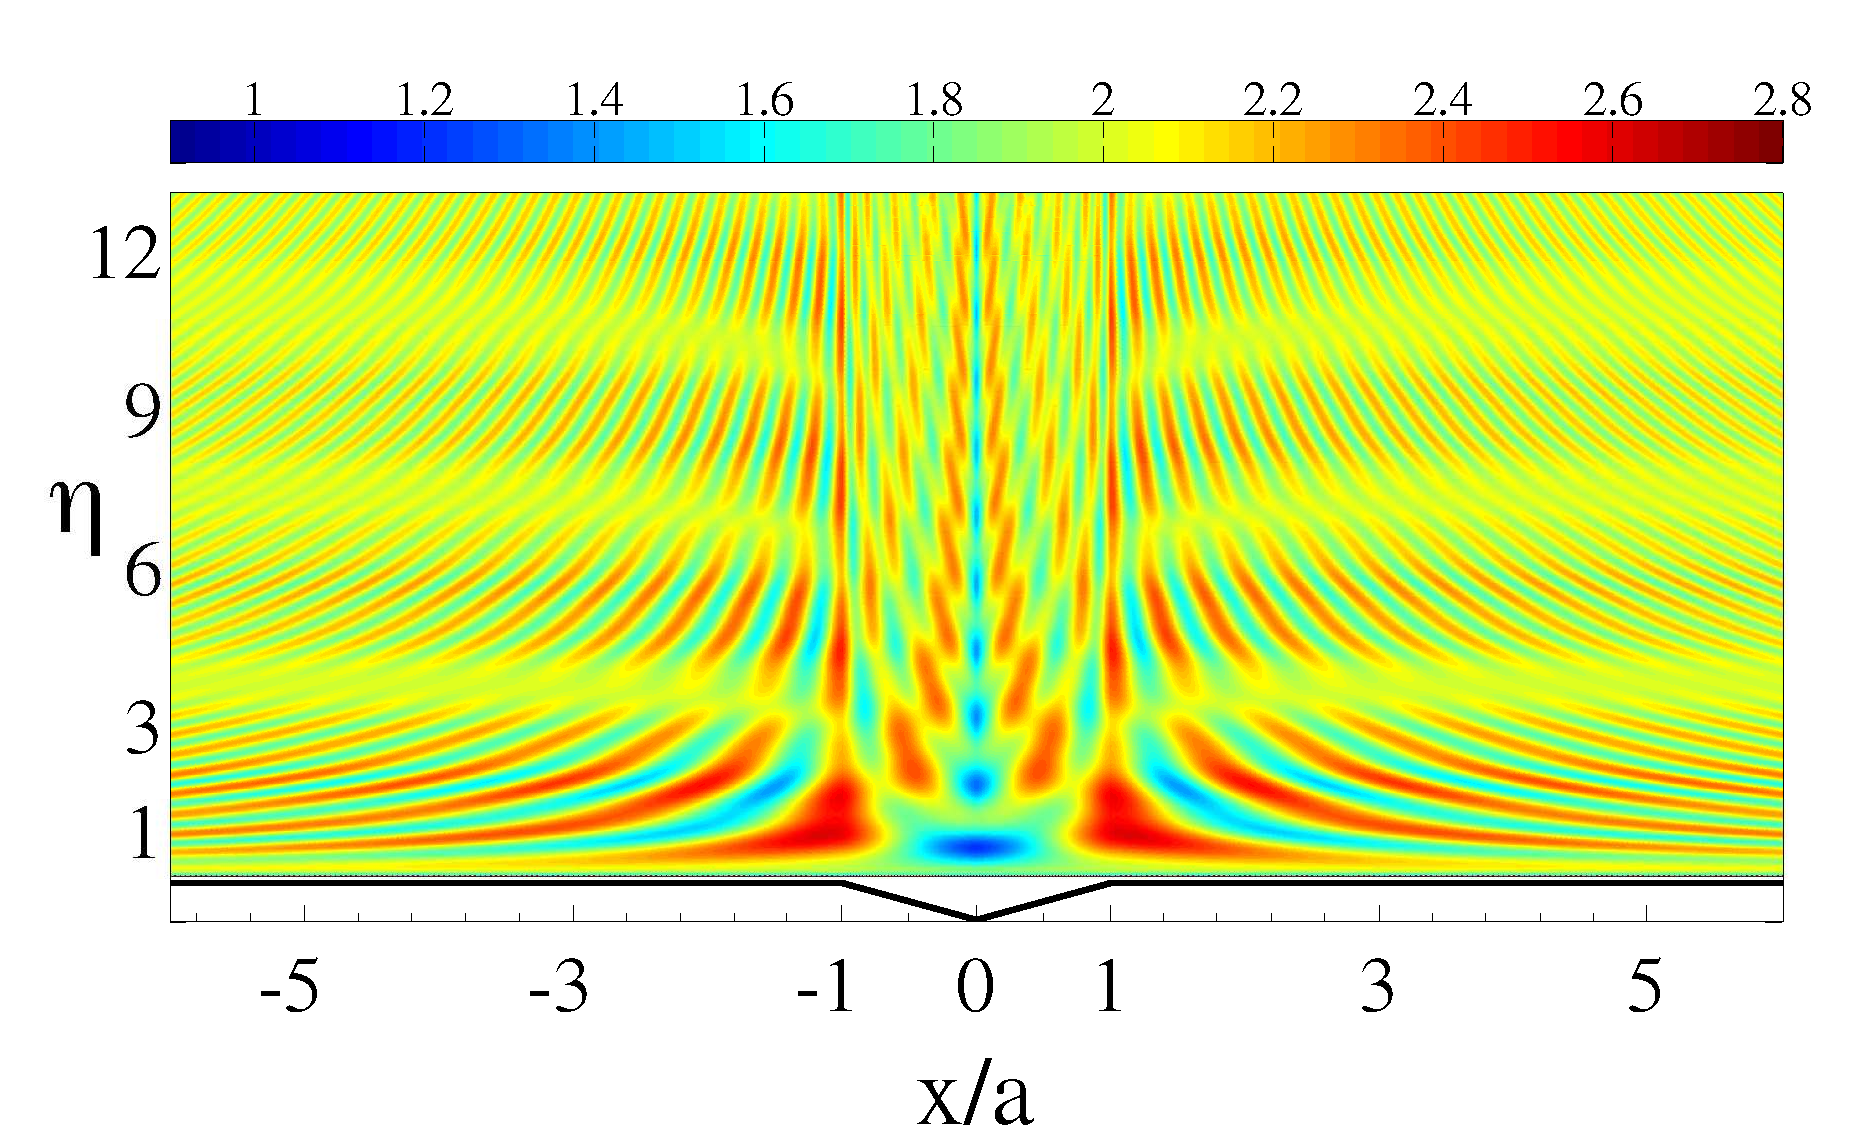
\includegraphics[width=0.7\linewidth]{IMAGES/Completo.pdf}}
%
	\begin{tabular}{cccc}
		\subfloat{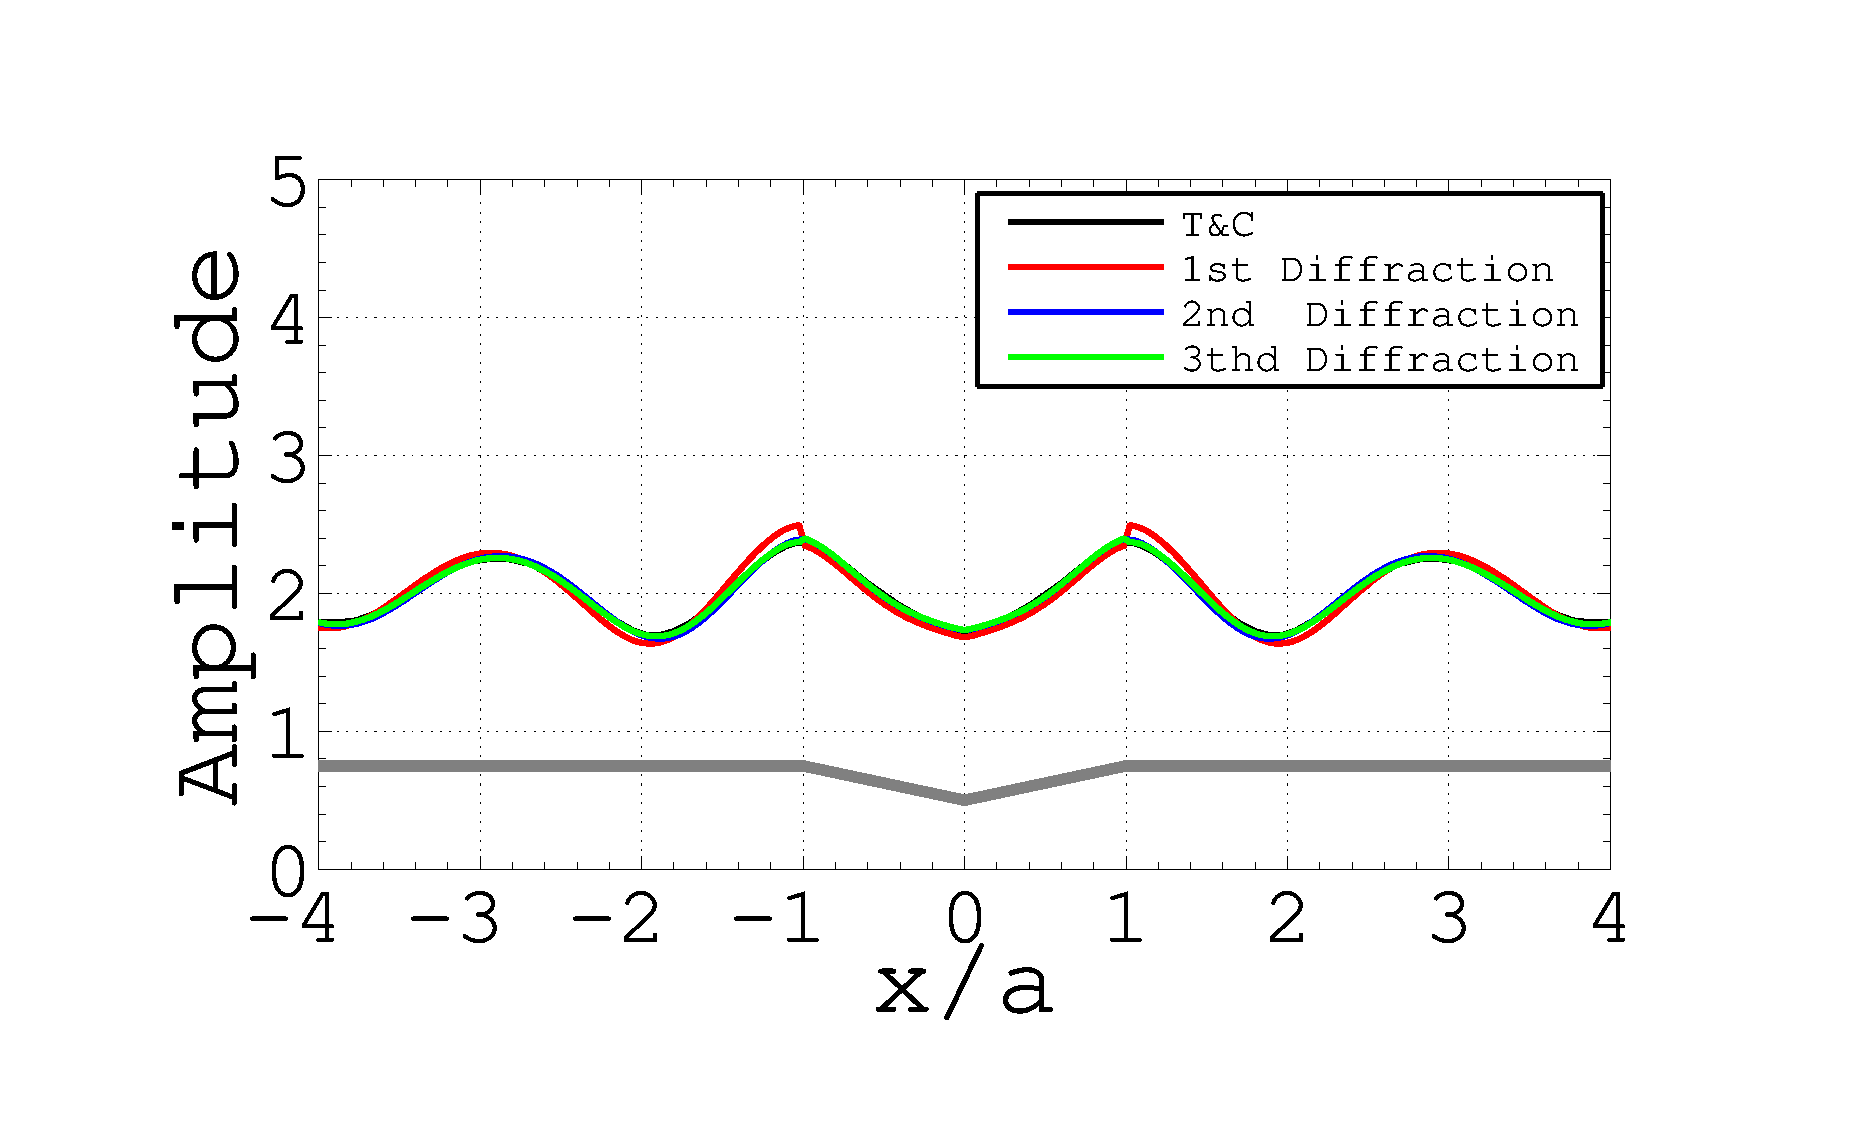
\includegraphics[width=5.0cm]{Figures/02_da_25_all.pdf}}
		\hspace{-1.5cm}
		& \subfloat{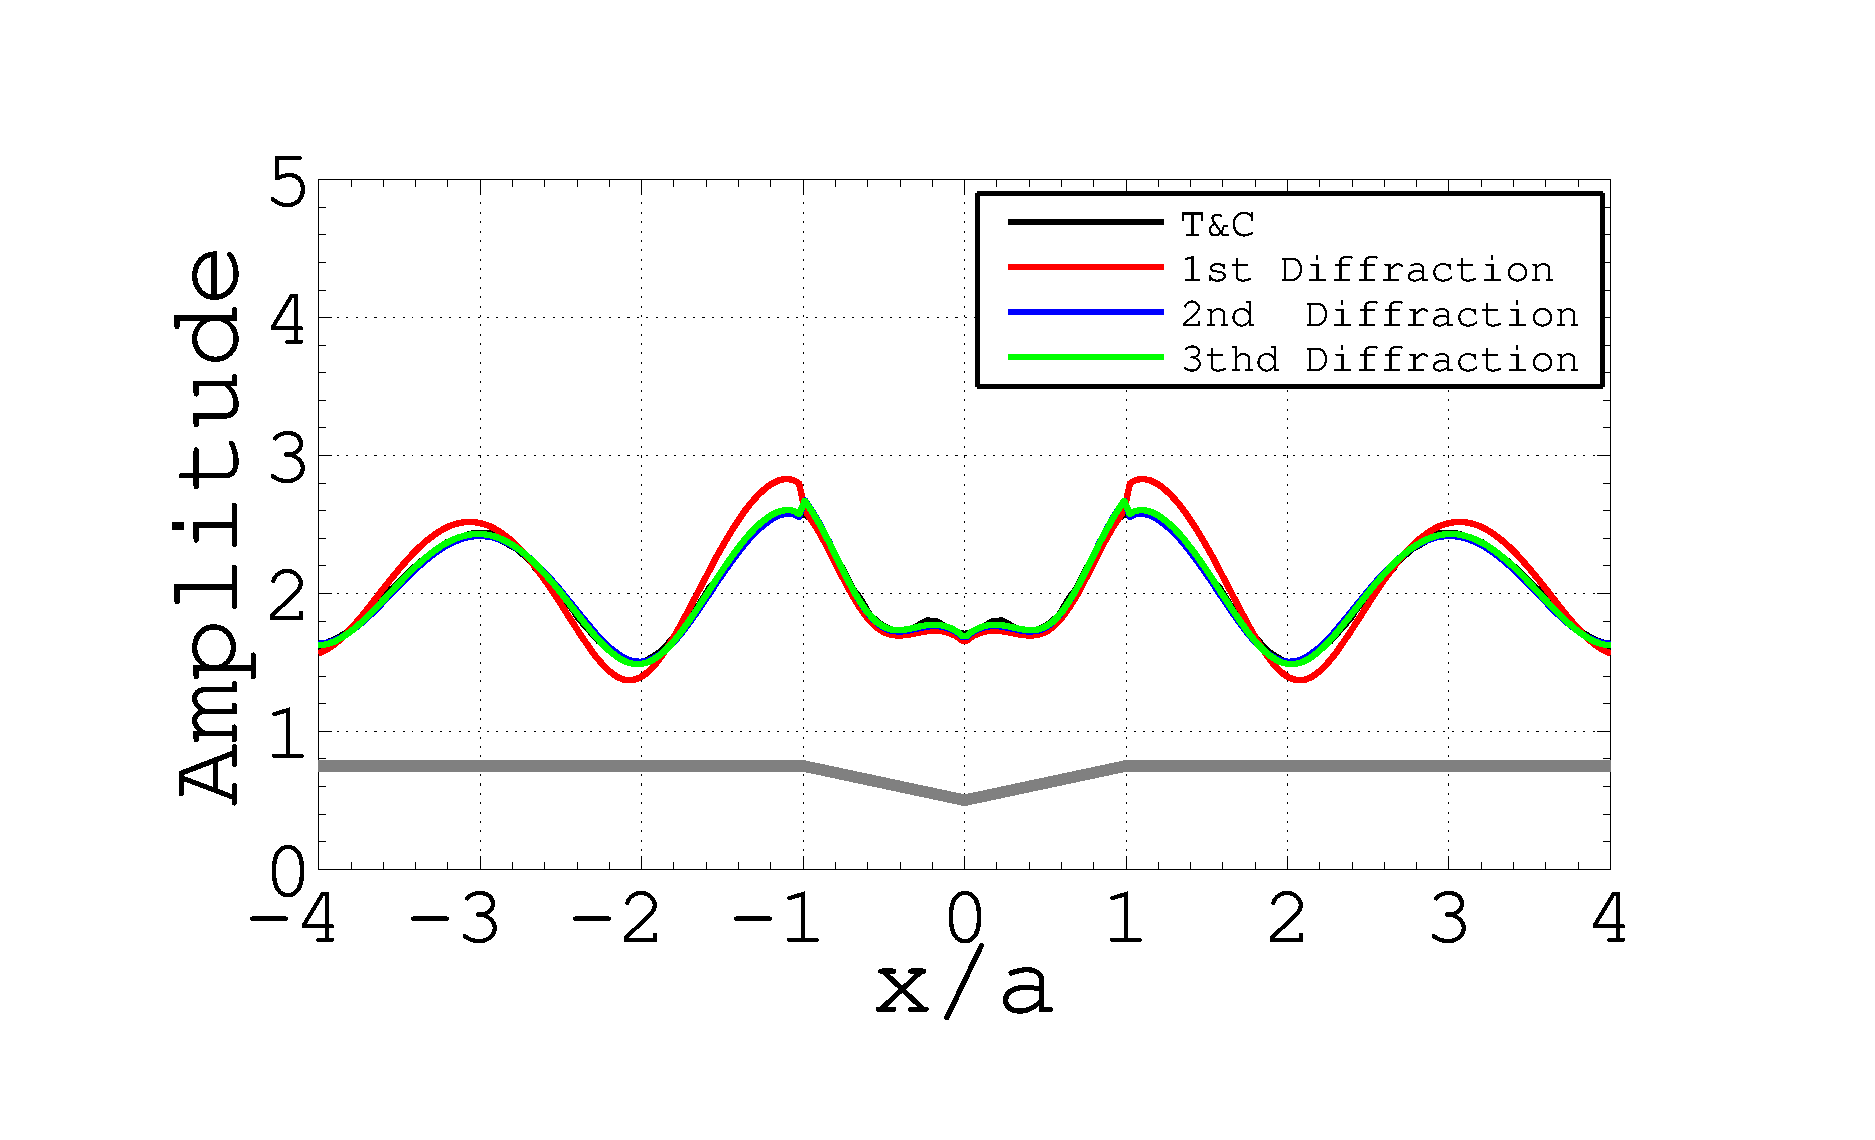
\includegraphics[width=5.0cm]{Figures/06_da_50_all.pdf}}
		\hspace{-1.5cm}
		& \subfloat{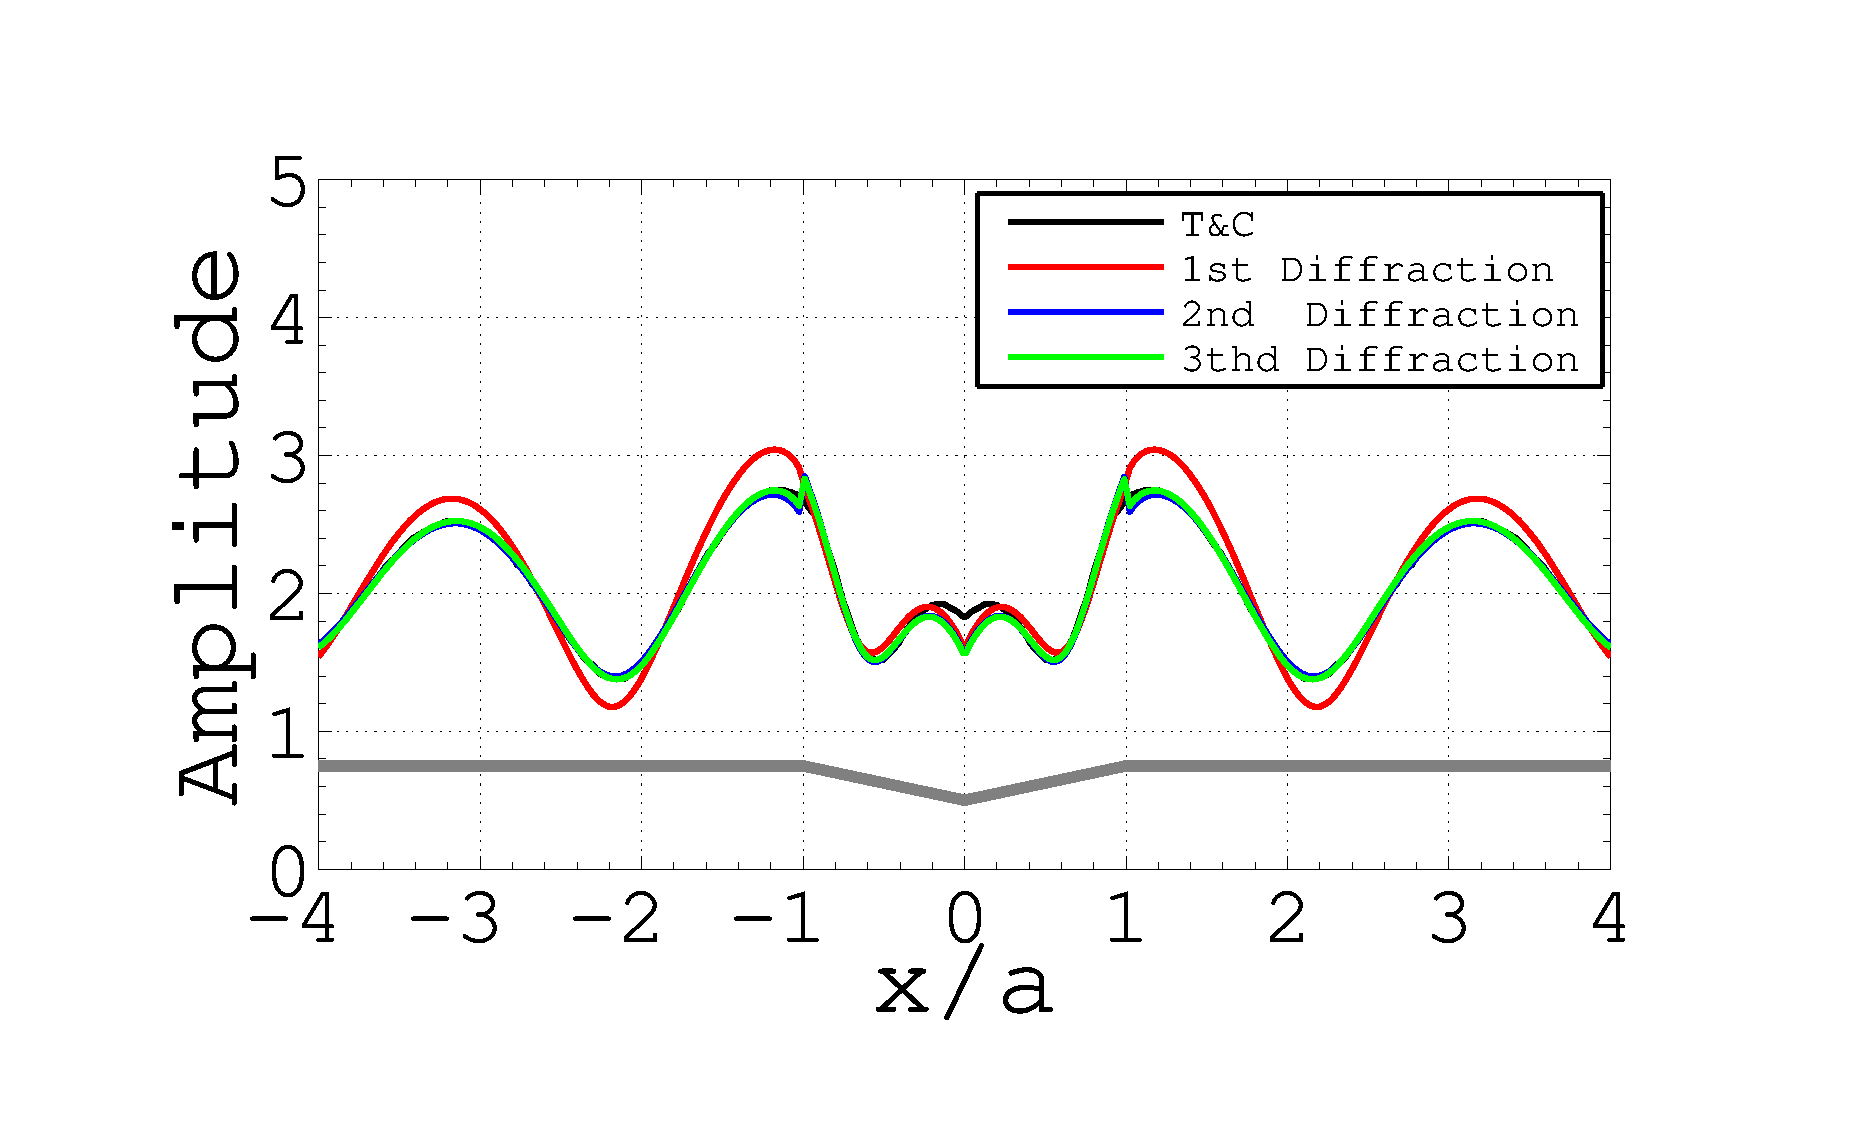
\includegraphics[width=5.0cm]{Figures/10_da_75_all.pdf}}
		\hspace{-1.5cm}
   		& \subfloat{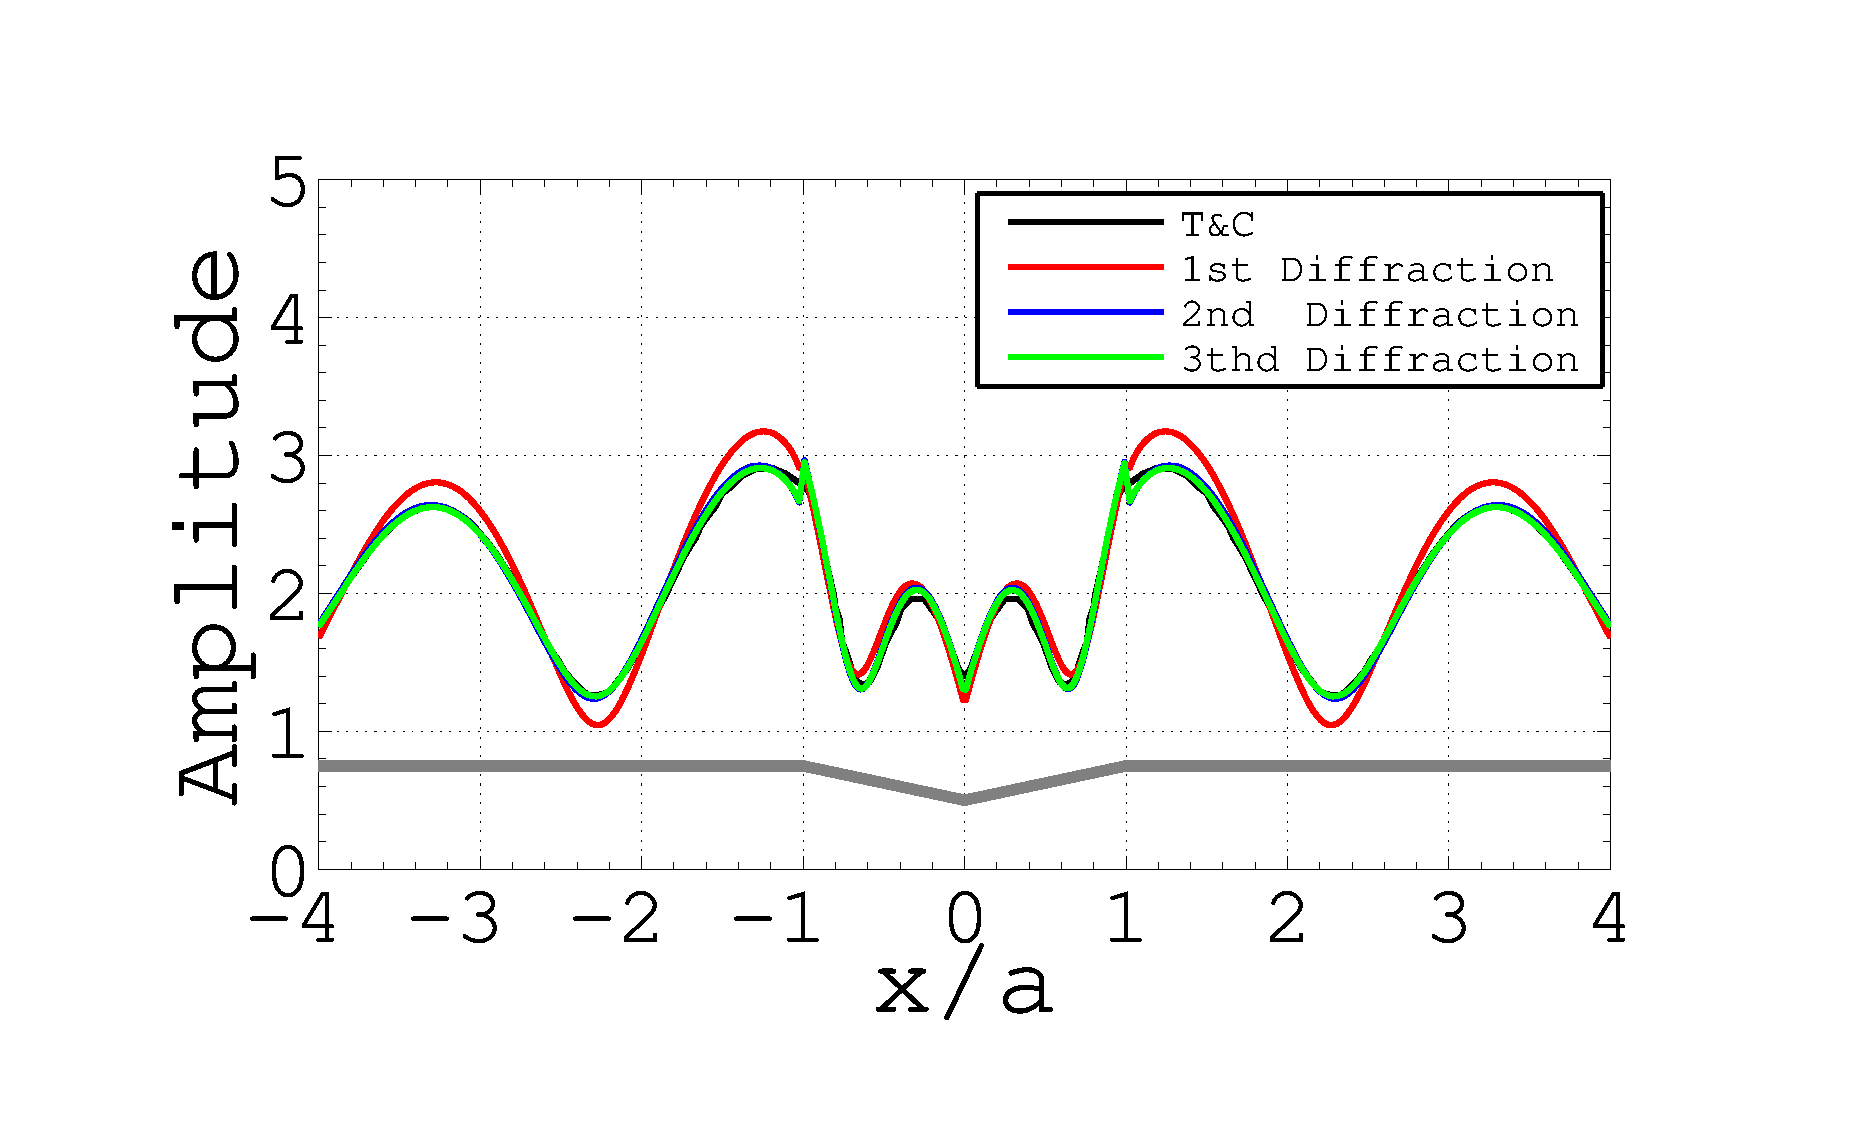
\includegraphics[width=5.0cm]{Figures/14_da_100_all.pdf}}
   		%
   		\vspace{-1 cm}\\	
		\subfloat{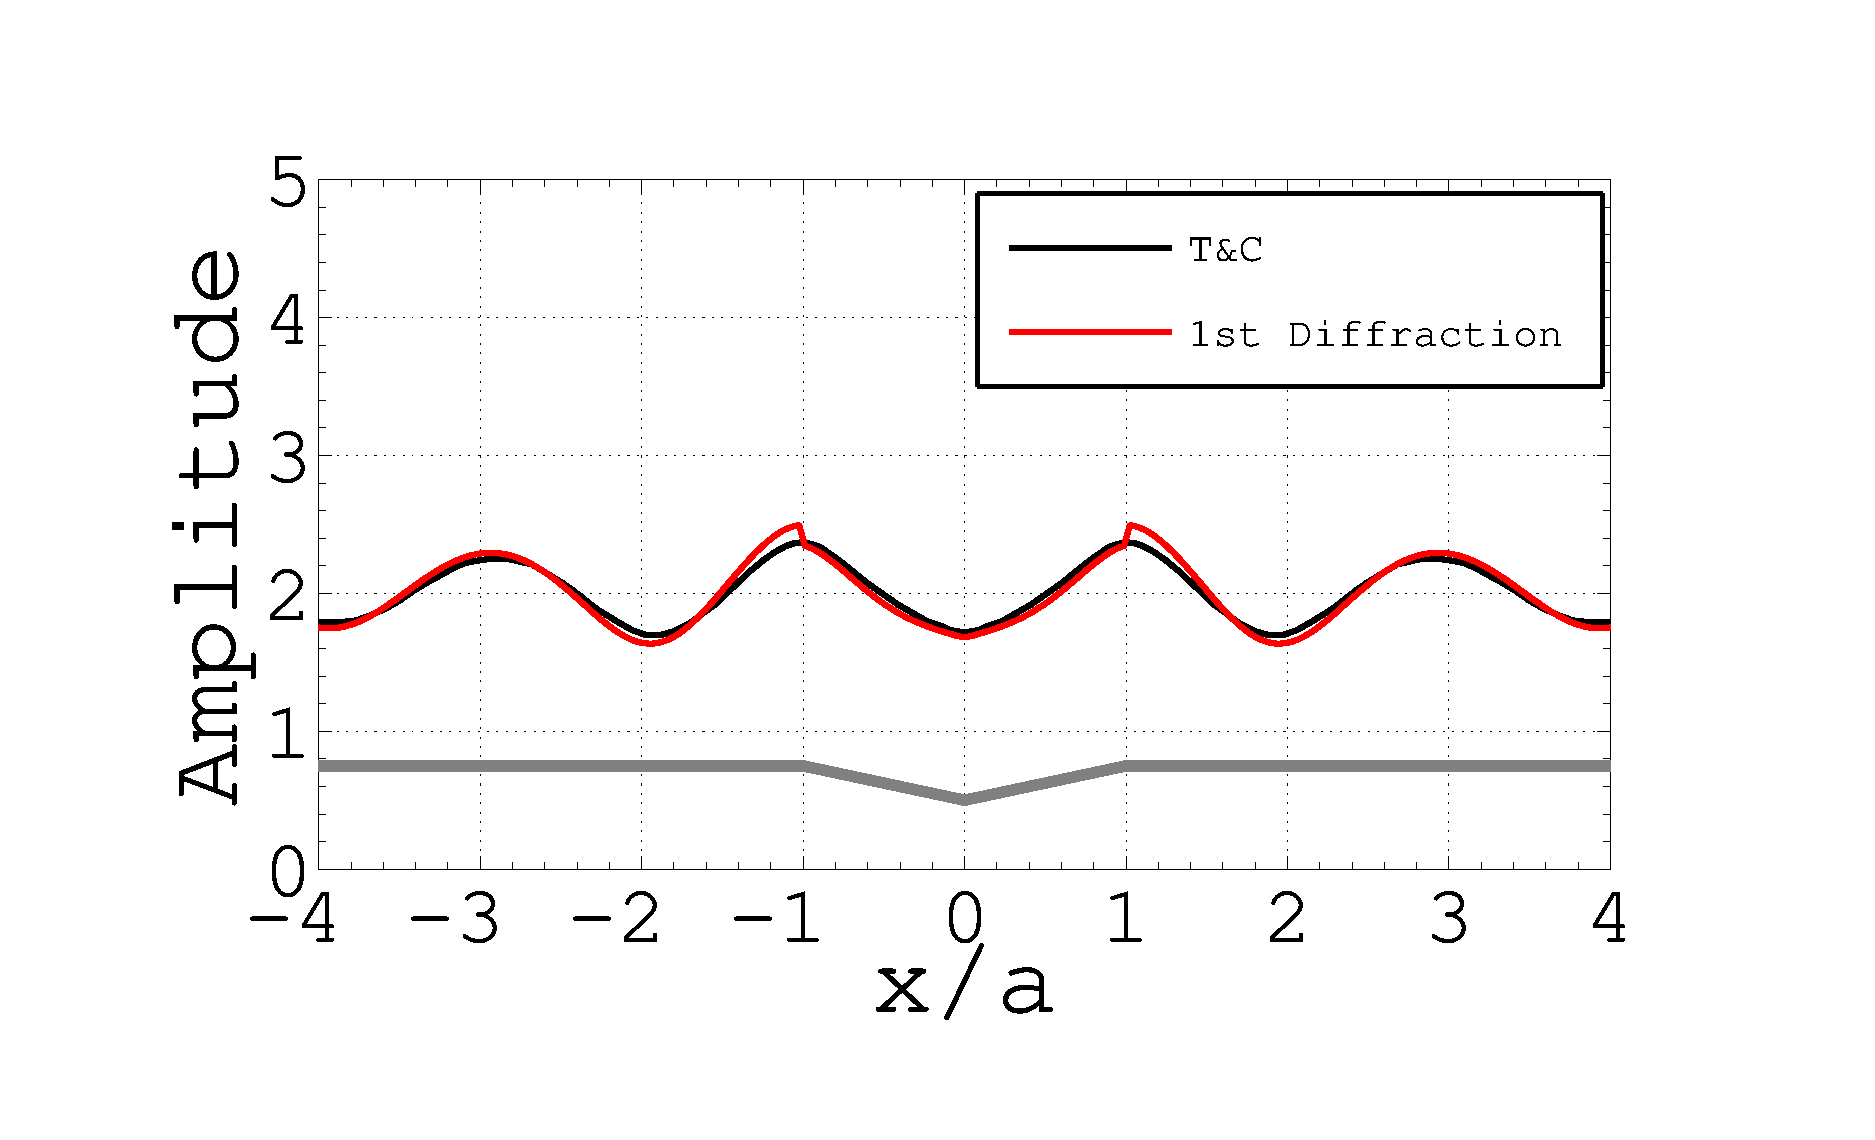
\includegraphics[width=5.0cm]{Figures/03_da_25_first.pdf}}
		\hspace{-1.5cm}
		& \subfloat{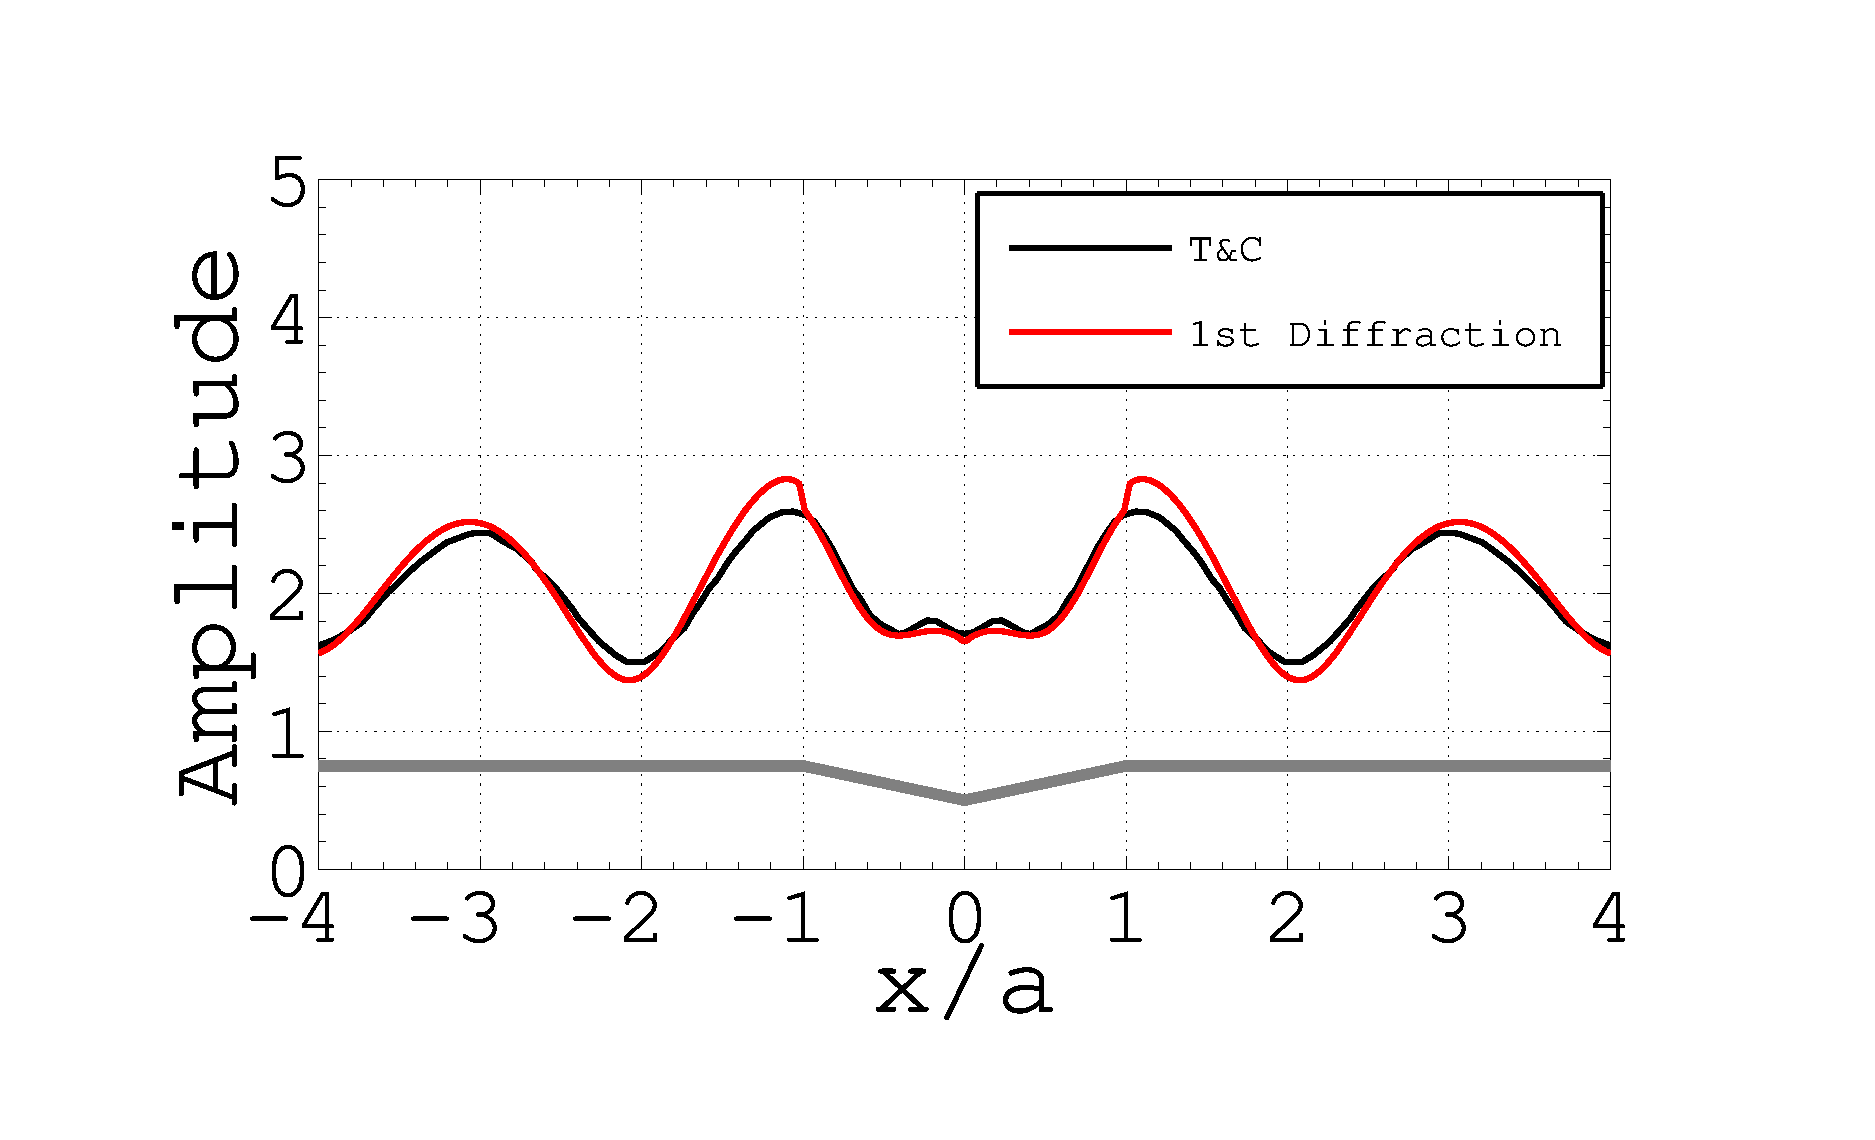
\includegraphics[width=5.0cm]{Figures/07_da_50_first.pdf}}
		\hspace{-1.5cm}
		& \subfloat{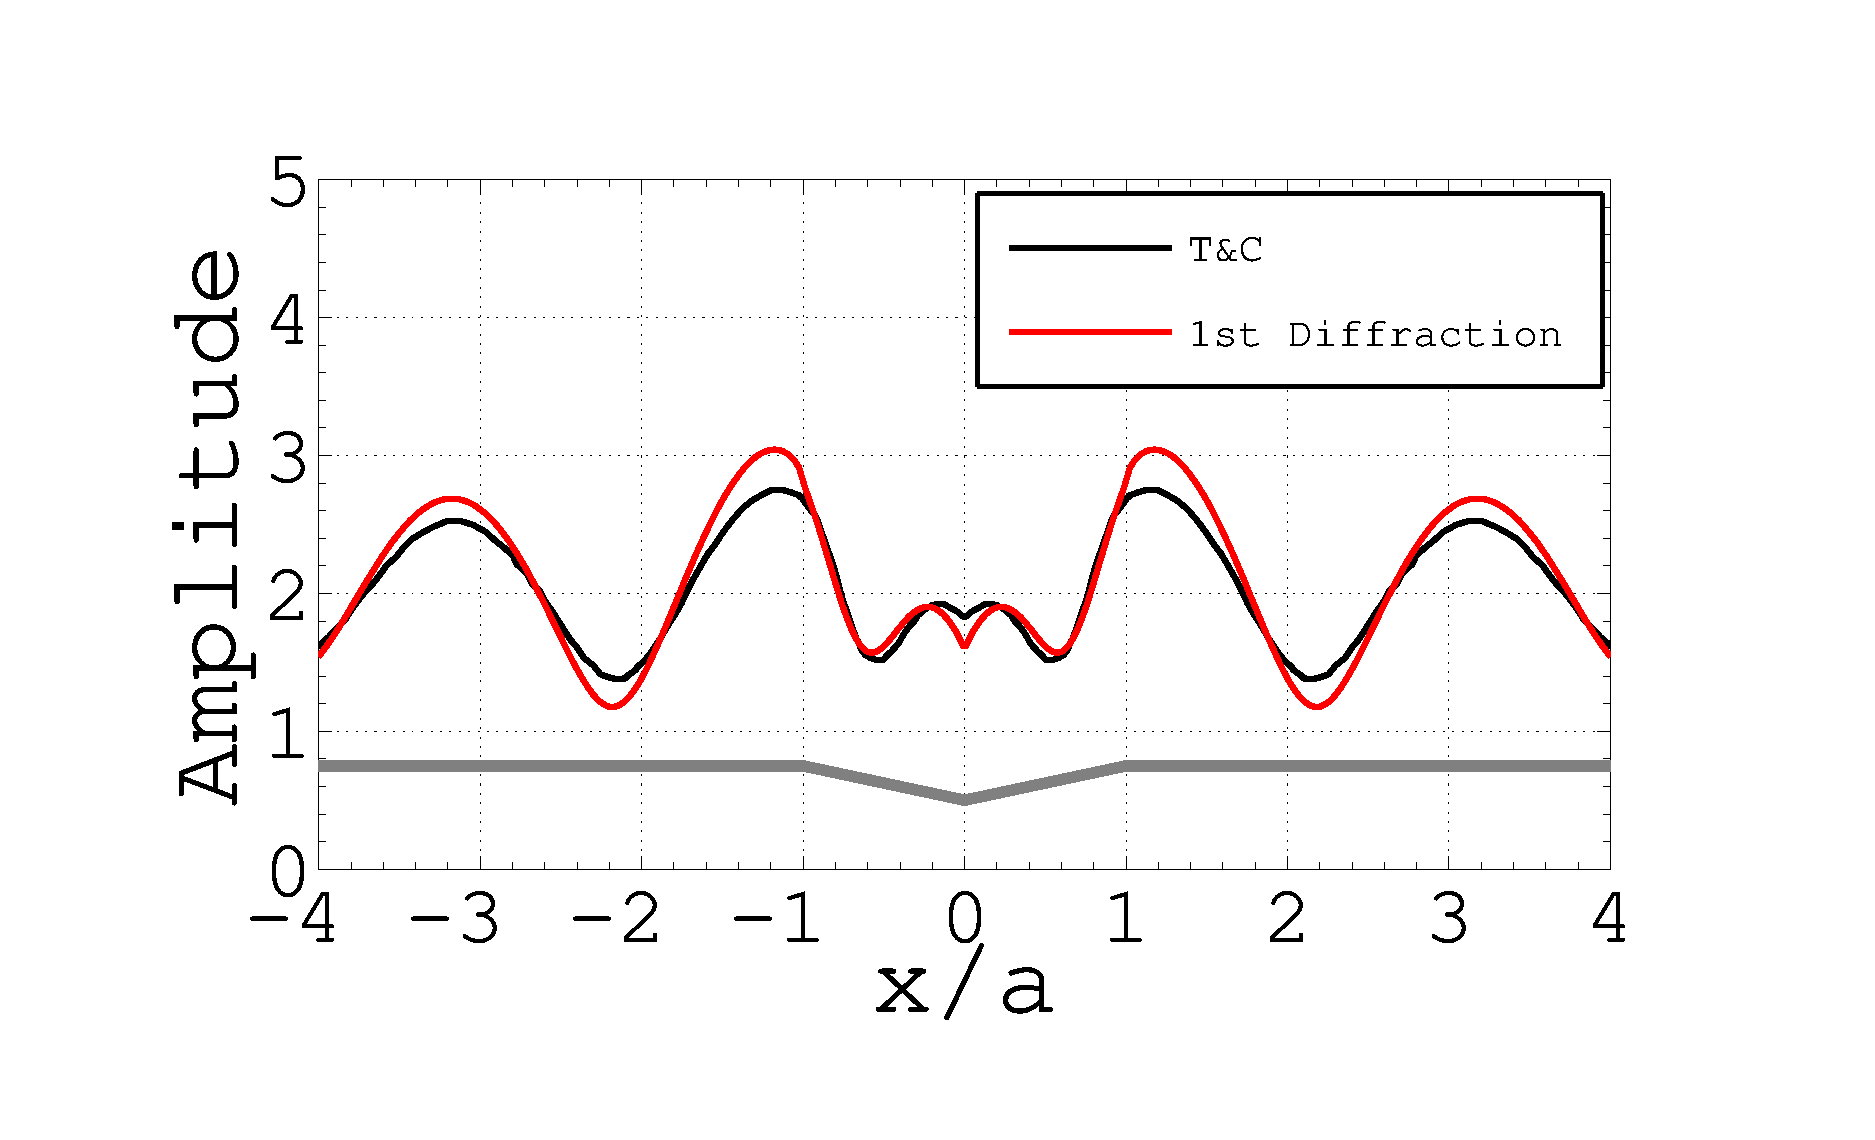
\includegraphics[width=5.0cm]{Figures/11_da_75_first.pdf}}
		\hspace{-1.5cm}
   		& \subfloat{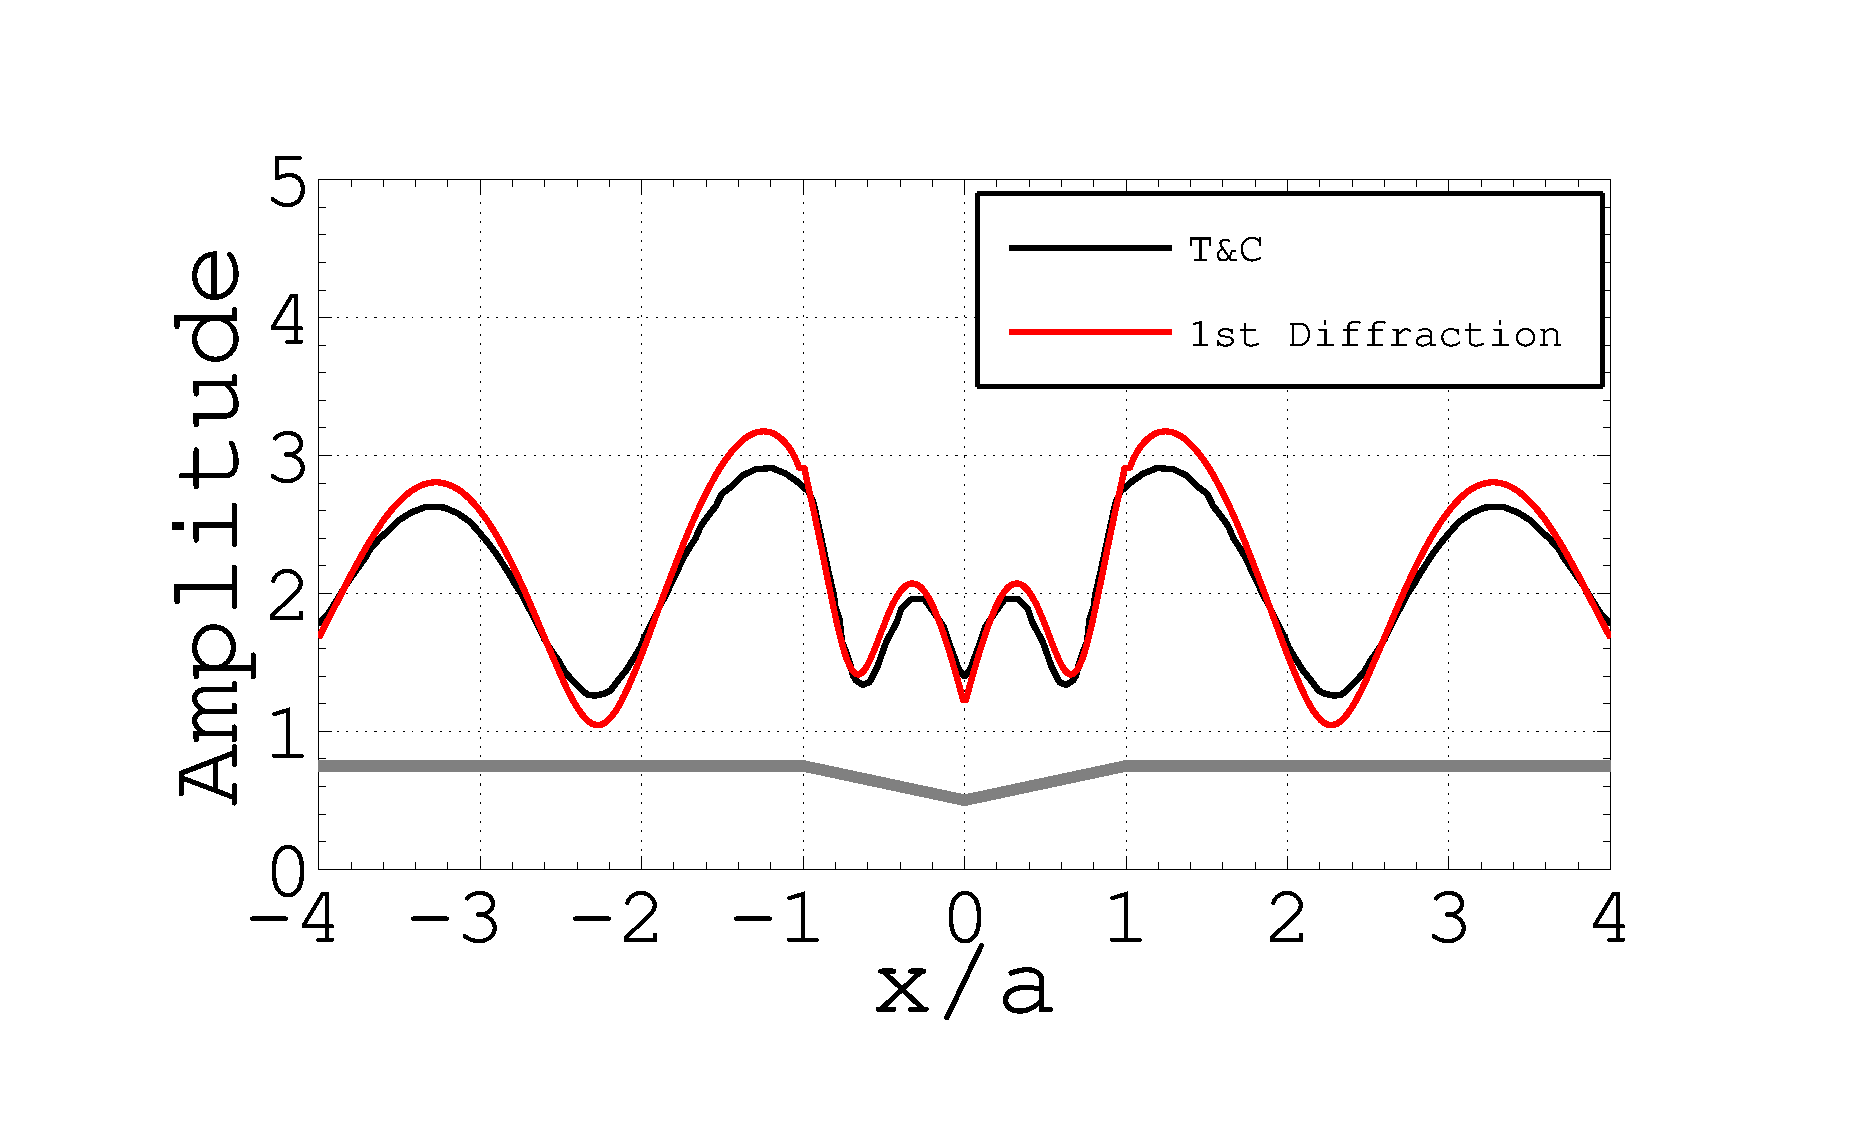
\includegraphics[width=5.0cm]{Figures/15_da_100_first.pdf}}
   		%
   		\vspace{-1 cm}\\	
		\subfloat{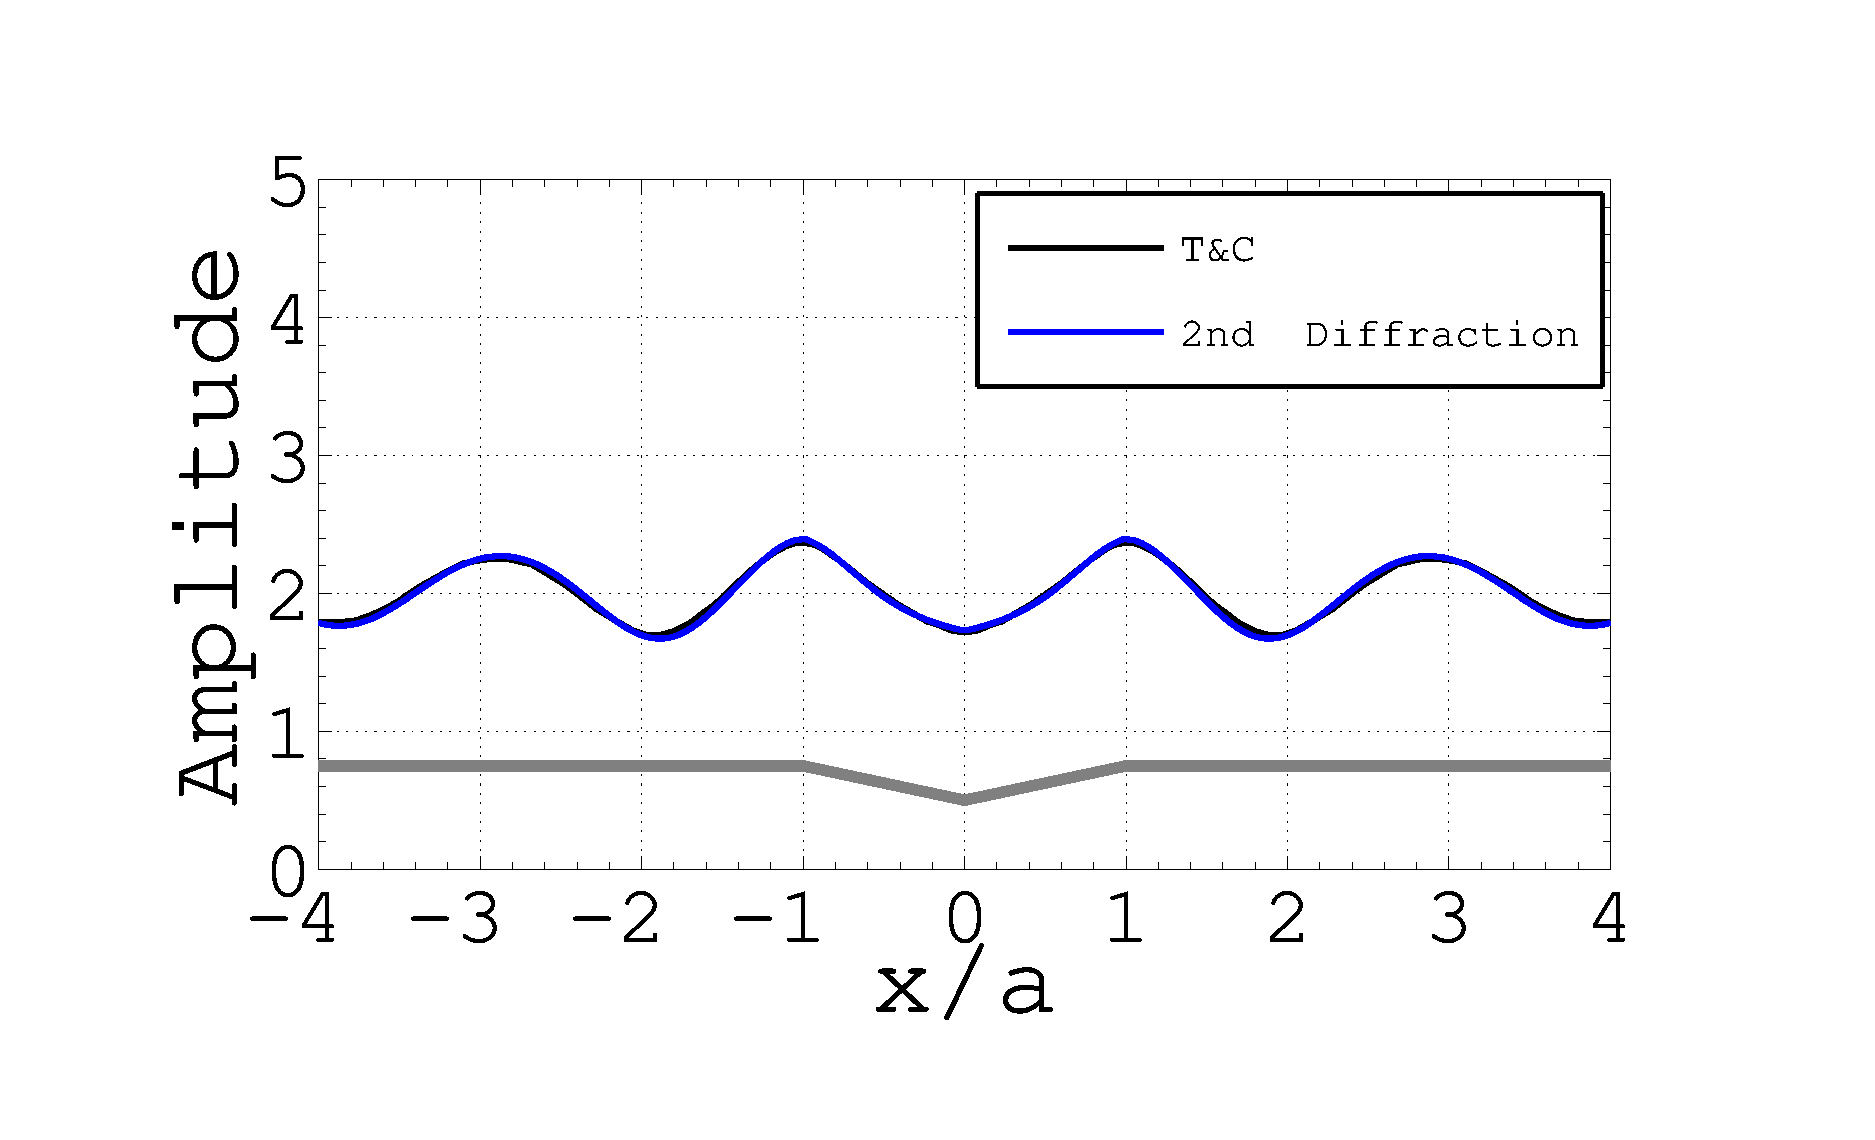
\includegraphics[width=5.0cm]{Figures/04_da_25_second.pdf}}
		\hspace{-1.5cm}
		& \subfloat{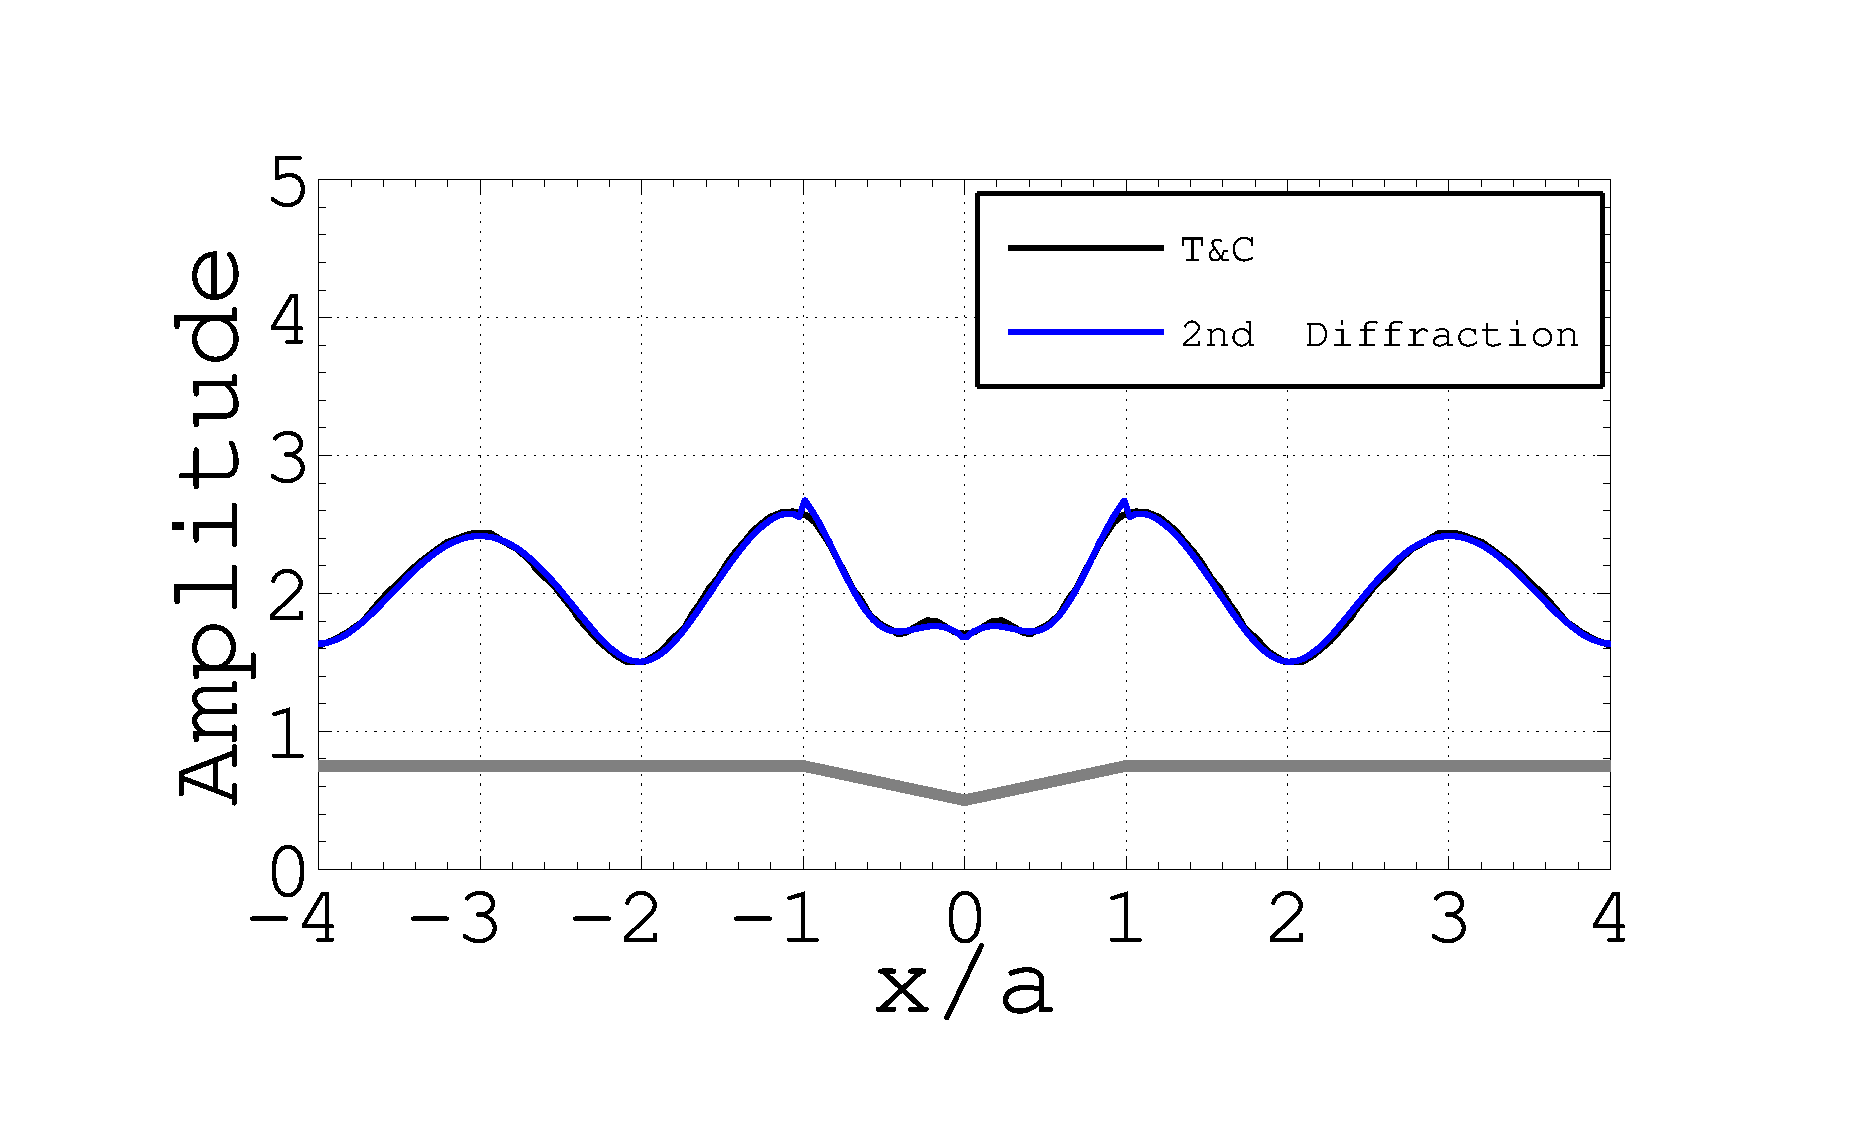
\includegraphics[width=5.0cm]{Figures/08_da_50_second.pdf}}
		\hspace{-1.5cm}
		& \subfloat{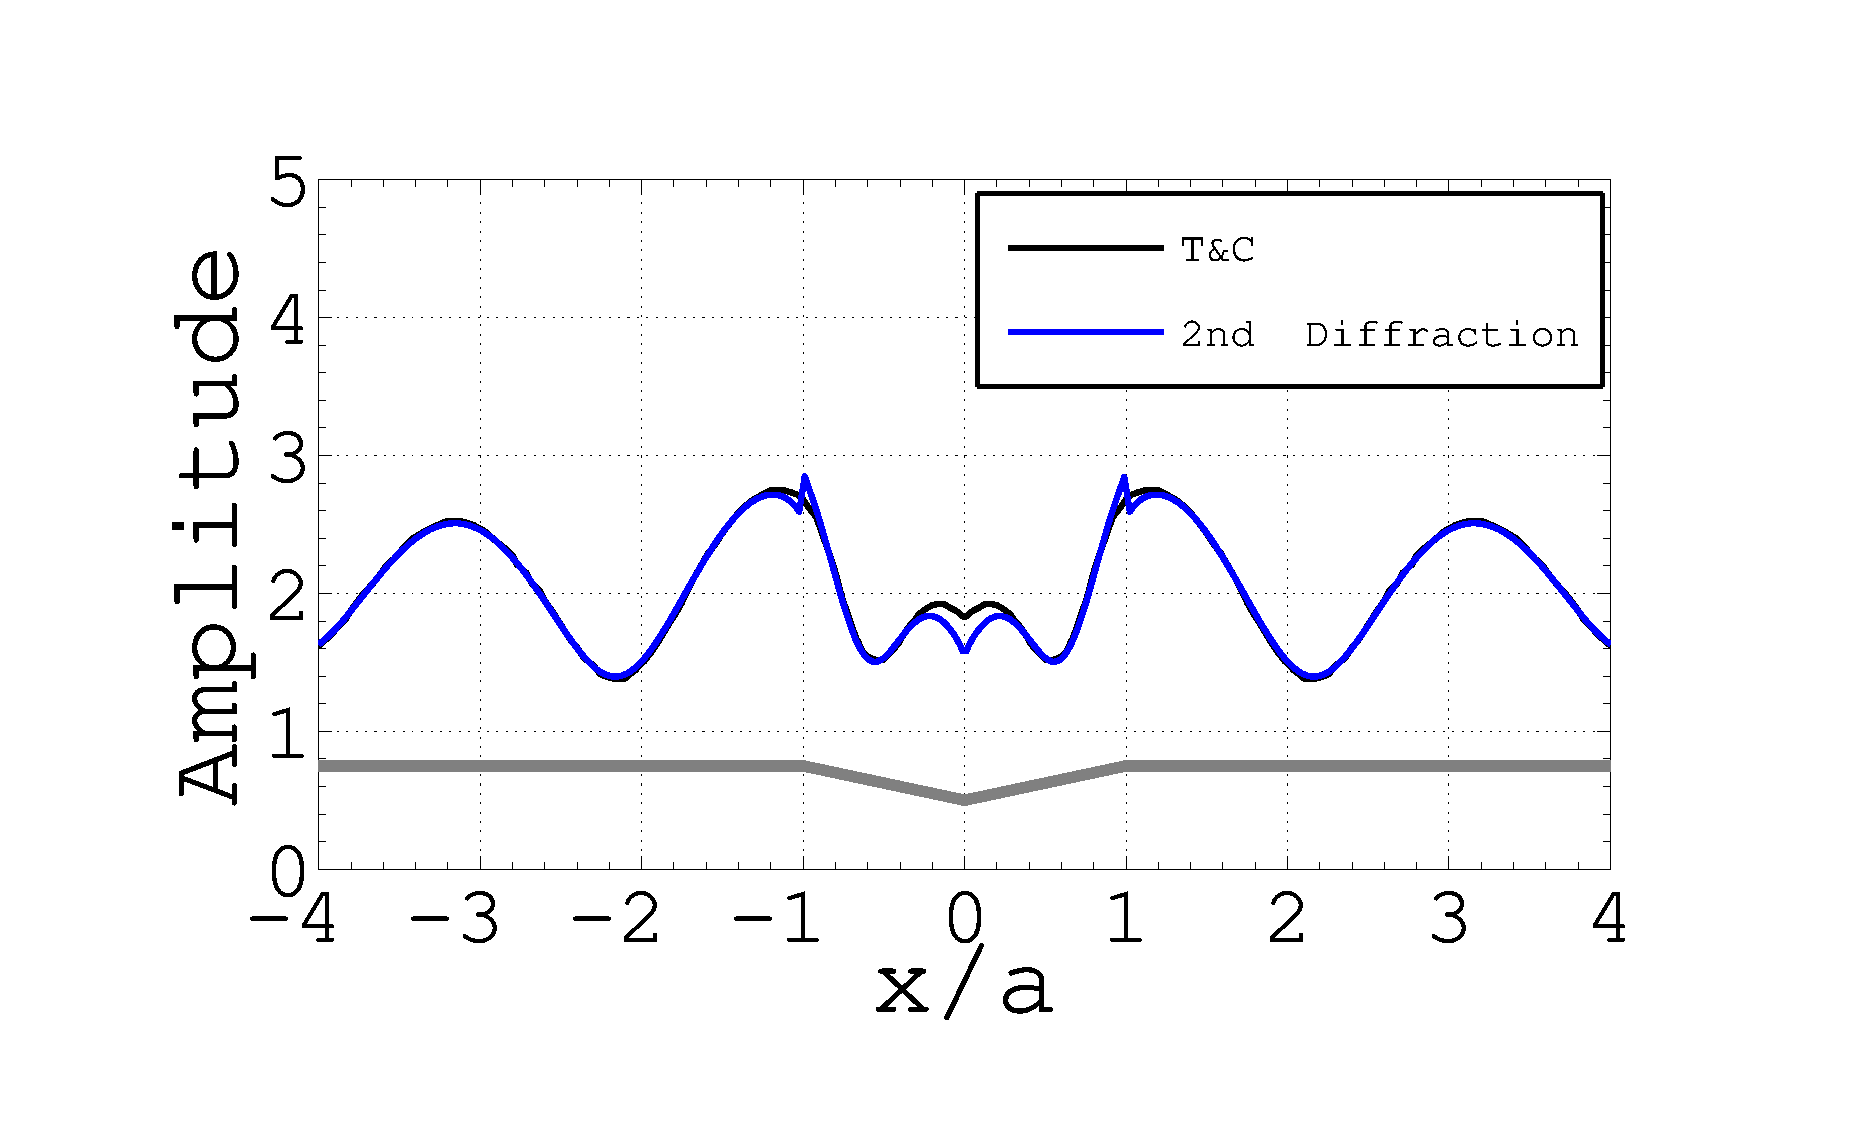
\includegraphics[width=5.0cm]{Figures/12_da_75_second.pdf}}
		\hspace{-1.5cm}
   		& \subfloat{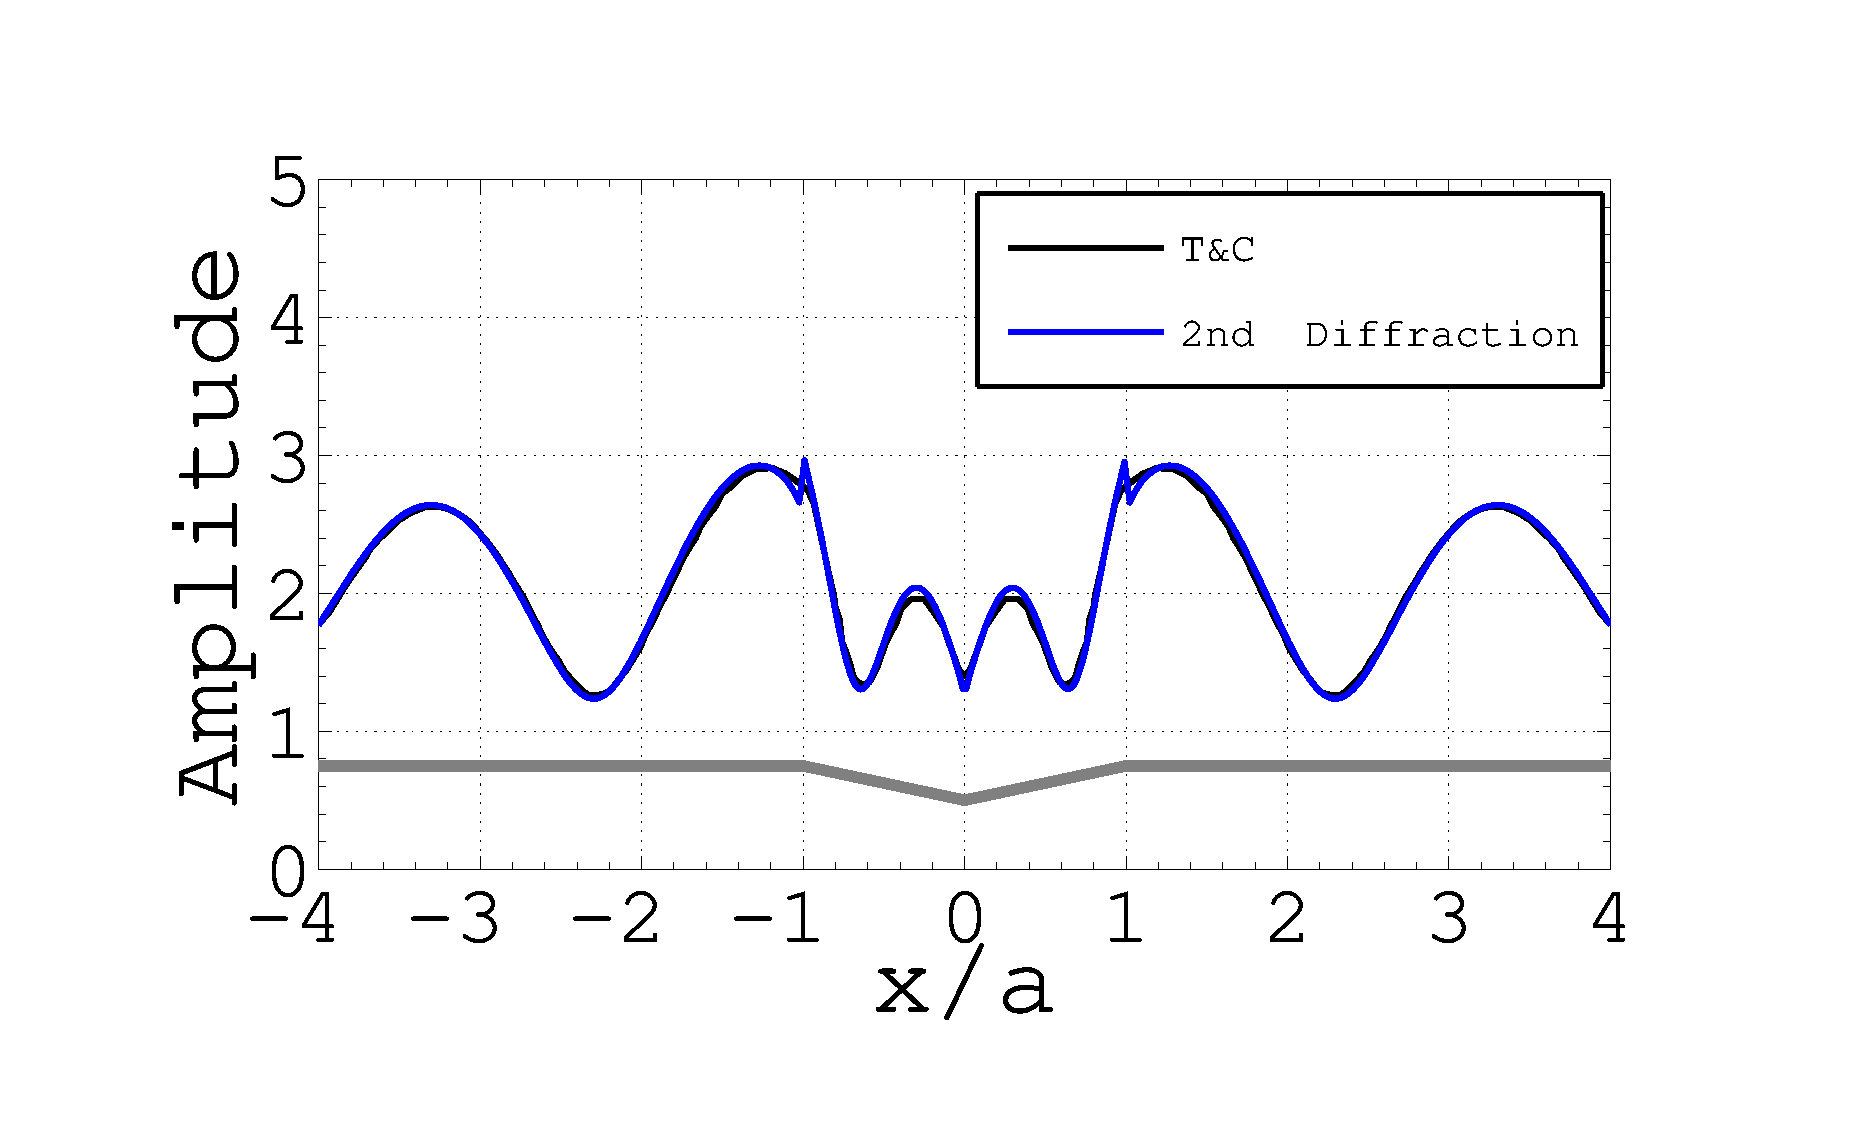
\includegraphics[width=5.0cm]{Figures/16_da_100_second.pdf}}
   		%
   		\vspace{-1 cm}\\	
		\subfloat[$d/a=0.25$]{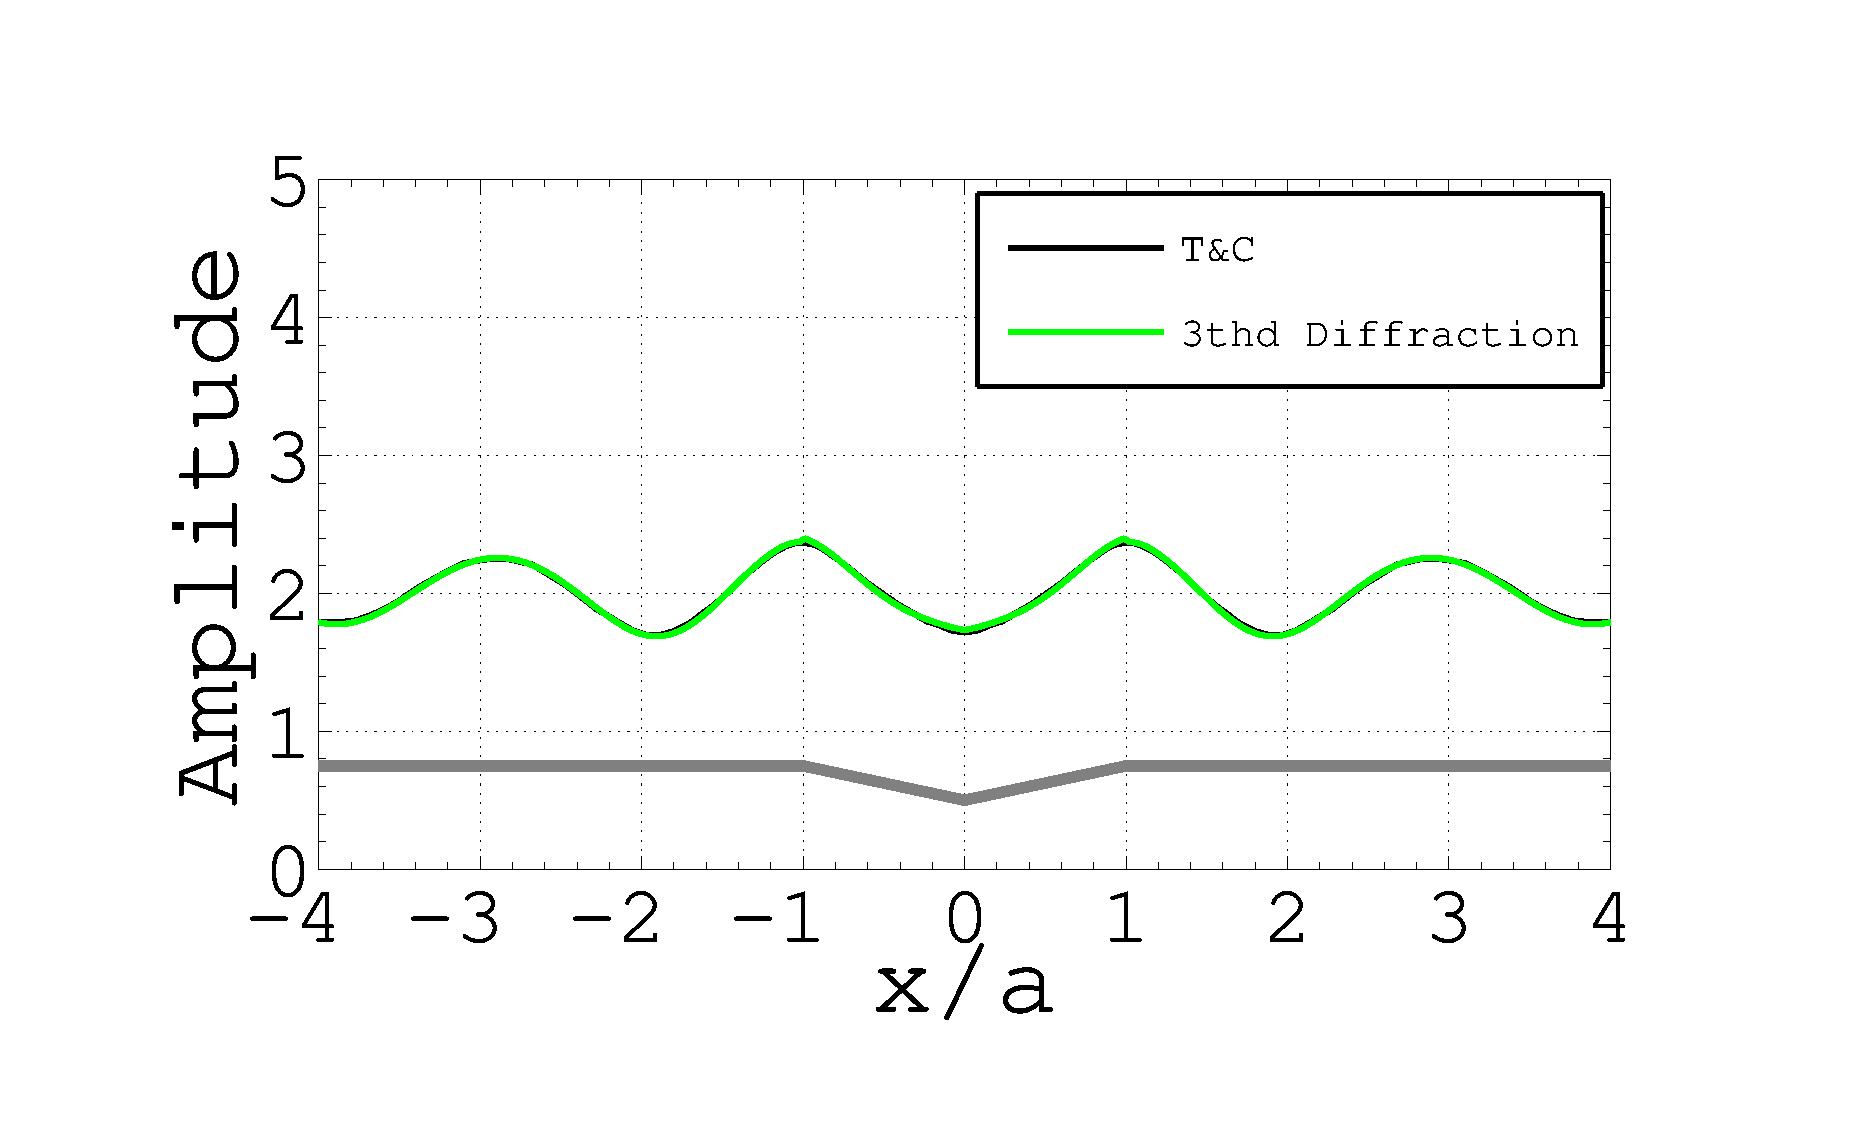
\includegraphics[width=5.0cm]{Figures/05_da_25_third.pdf}}
		\hspace{-1.5cm}
		& \subfloat[$d/a=0.50$]{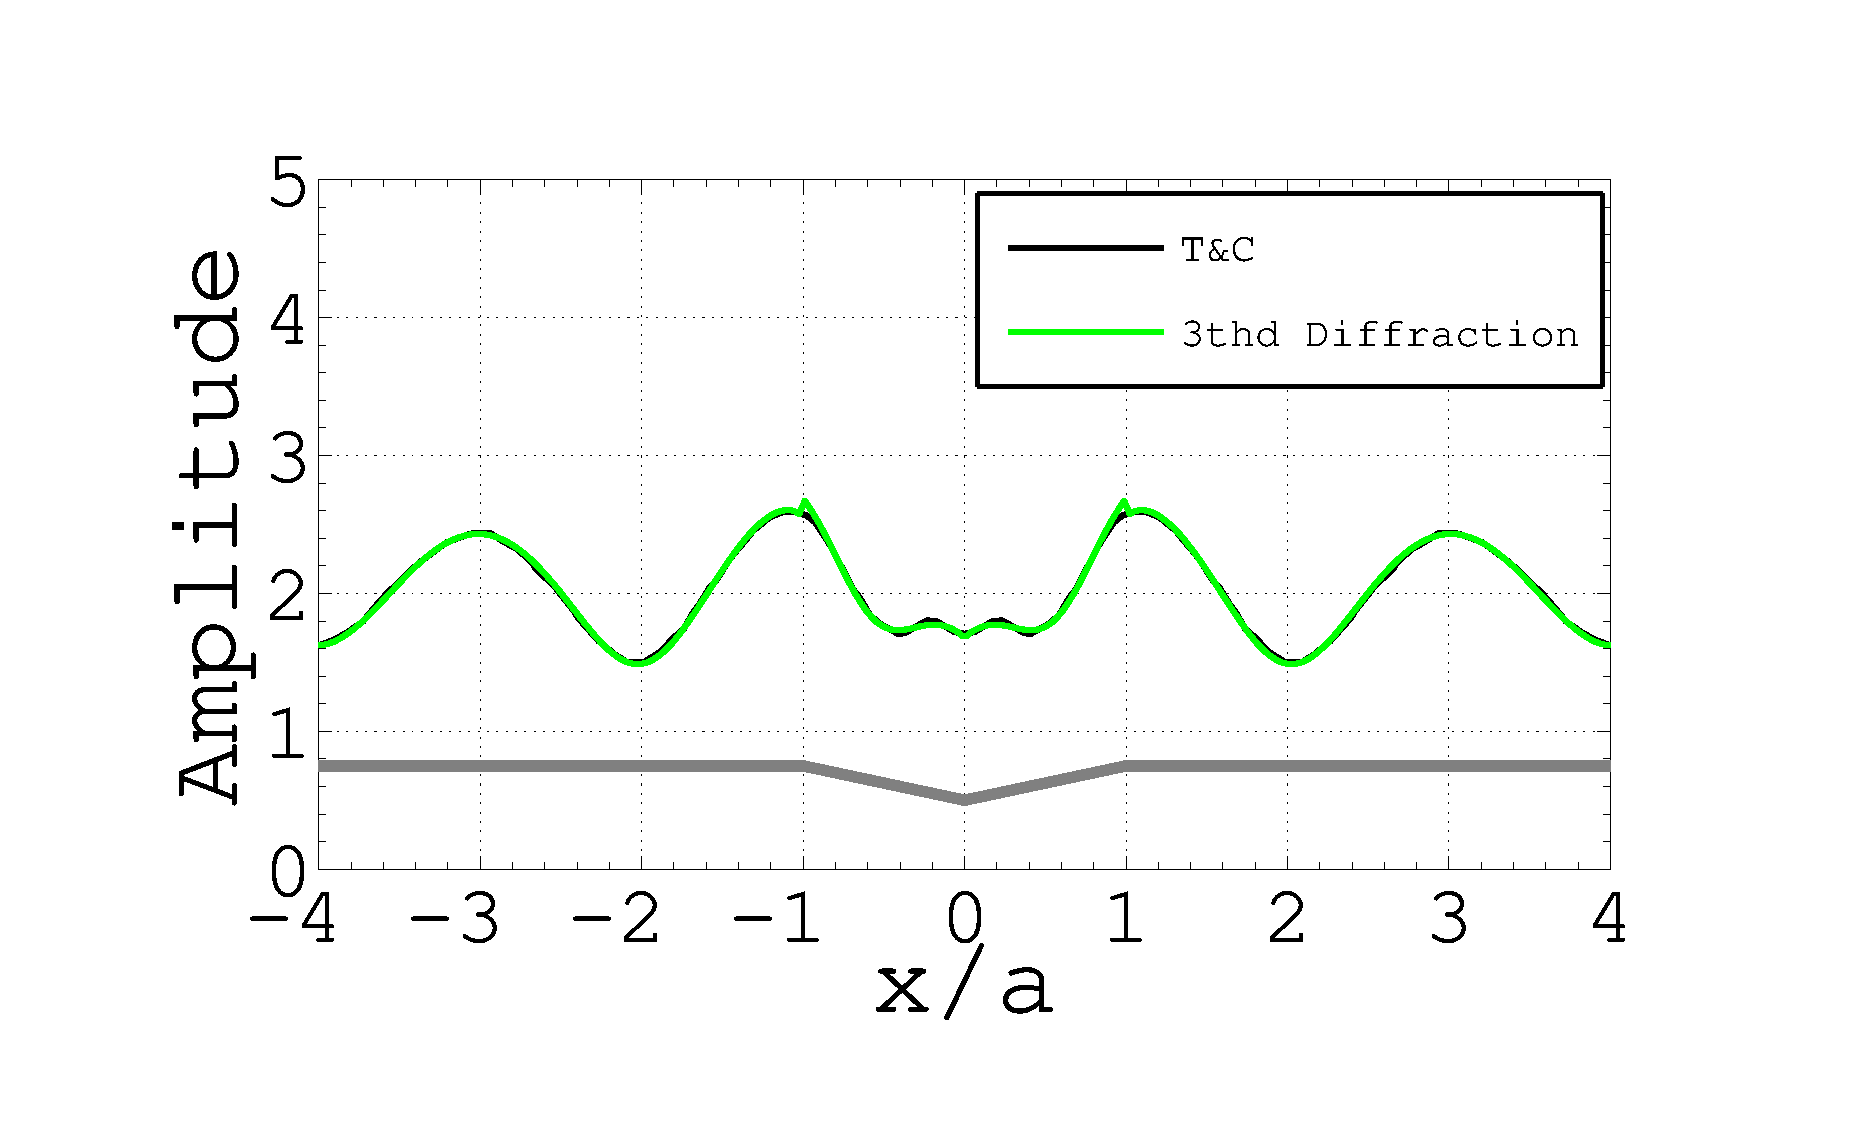
\includegraphics[width=5.0cm]{Figures/09_da_50_third.pdf}}
		\hspace{-1.5cm}
		& \subfloat[$d/a=0.75$]{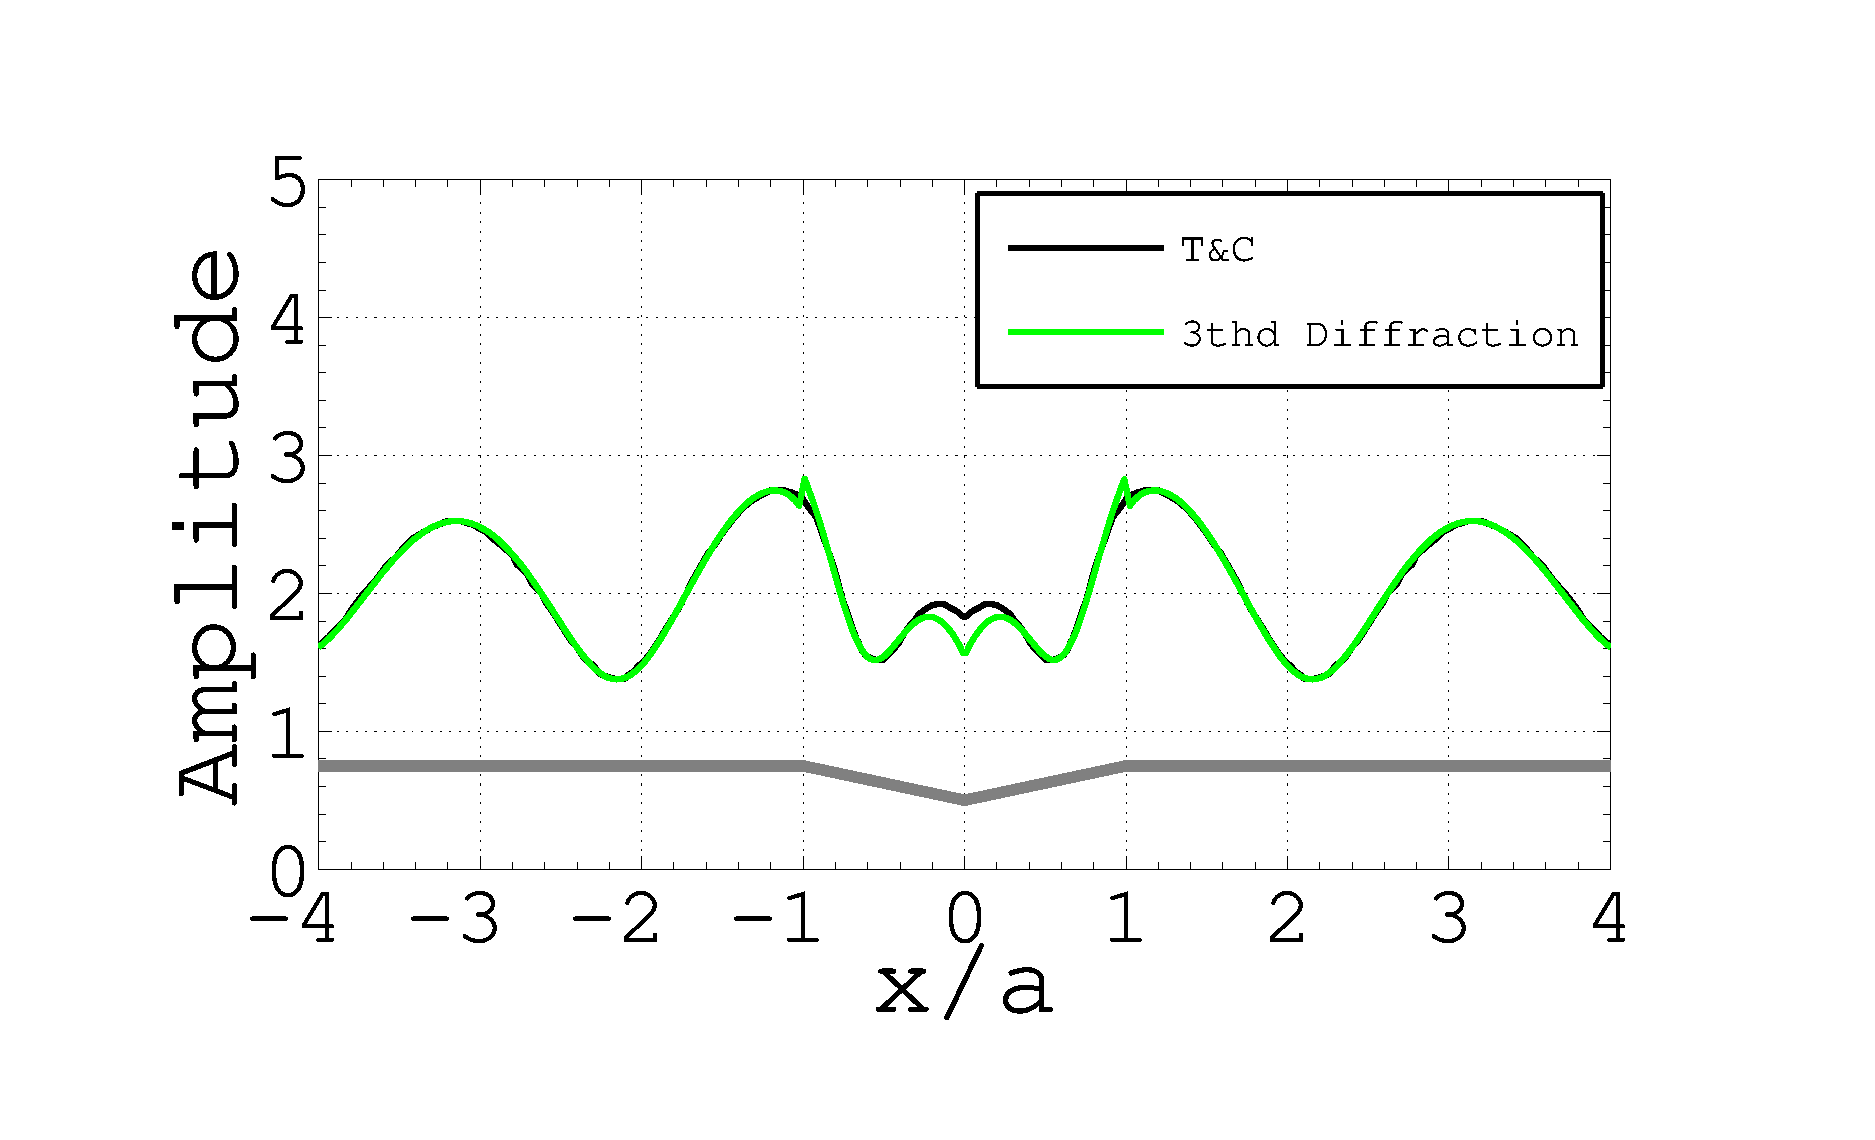
\includegraphics[width=5.0cm]{Figures/13_da_75_third.pdf}}
		\hspace{-1.5cm}
   		& \subfloat[$d/a=1.00$]{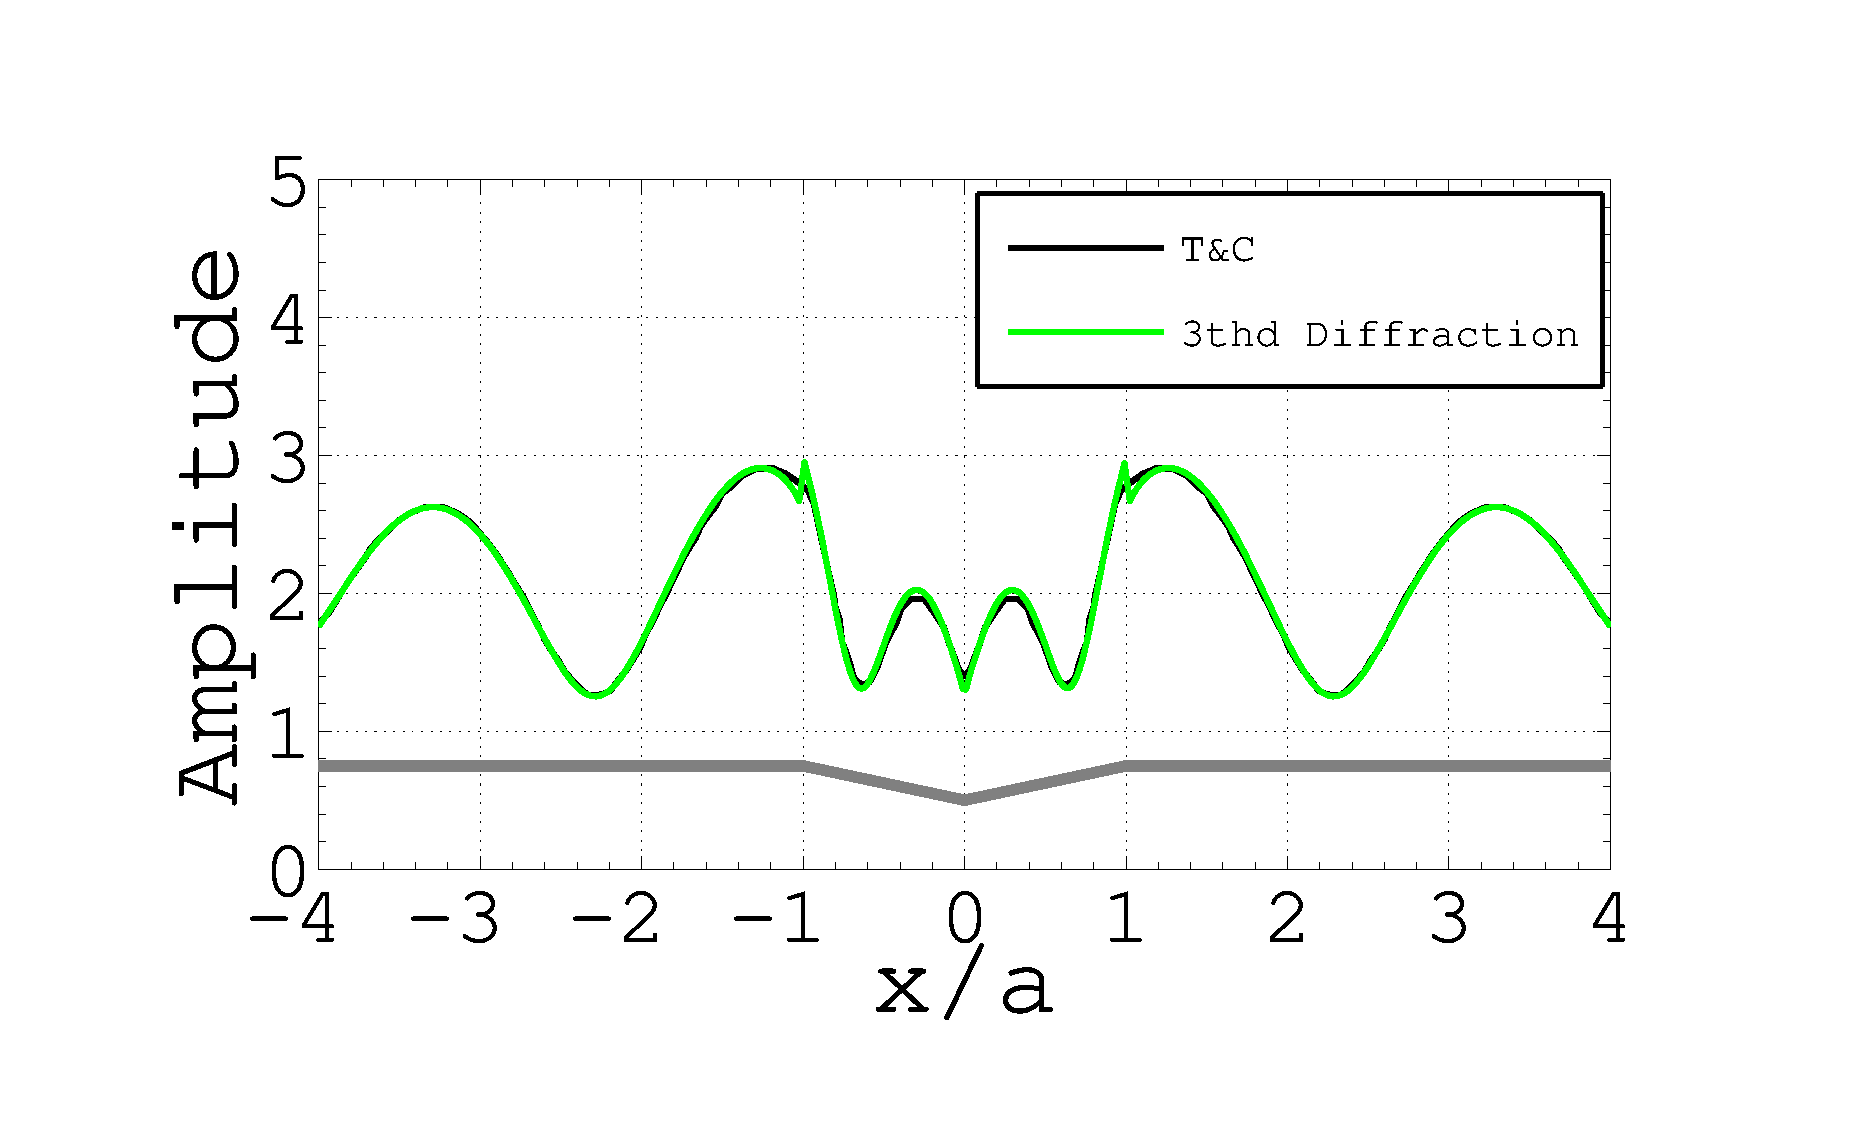
\includegraphics[width=5.0cm]{Figures/17_da_100_third.pdf}}\\
   		
	\end{tabular}
%tsaur2008analytical
%\end{tabularx}
\caption{Spatial distribution of the amplitude response function over the free-surface of a symmetrical $V$-shaped canyon with depth-to-width aspect ratio $d/a=0.25, 0.50, 0.75, 1.00$ and dimensionless frequency $\eta=1.00$. The first row compares the solution for each aspect ratio obtained by the region matching technique reported in \cite{tsaur2008analytical} (T\&C) and the SBD approach (this work) with 1, 2 and 3 orders of diffraction.}\label{fig:SBD_Tsaur}
\end{figure}
\end{landscape}



\begin{landscape}
\begin{figure}
\def\tabularxcolumn#1{m{#1}}
%\begin{tabularx}{\linewidth}{@{}Xc@{}}
%
%\subfloat[BEM]{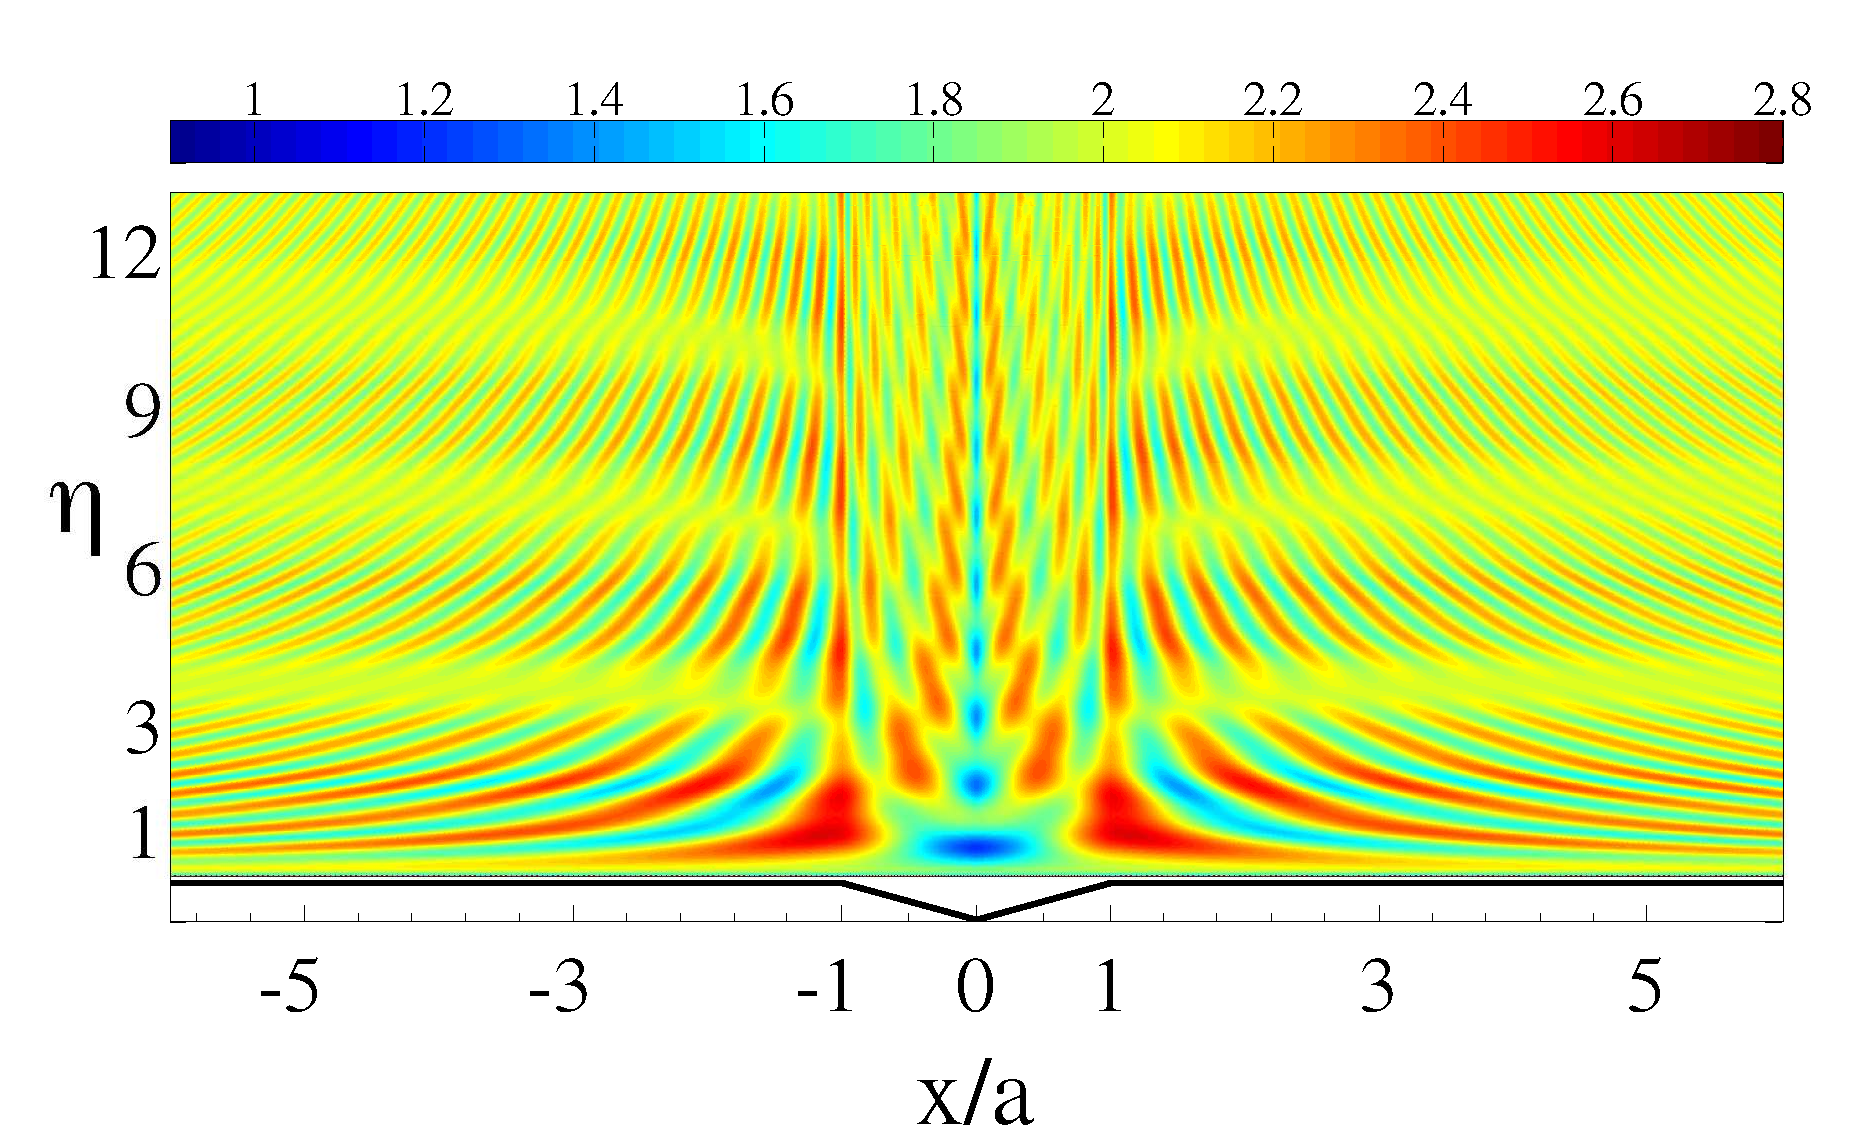
\includegraphics[width=0.7\linewidth]{IMAGES/Completo.pdf}}
%
	\begin{tabular}{cccc}
		\subfloat[$x/a=0.50$]{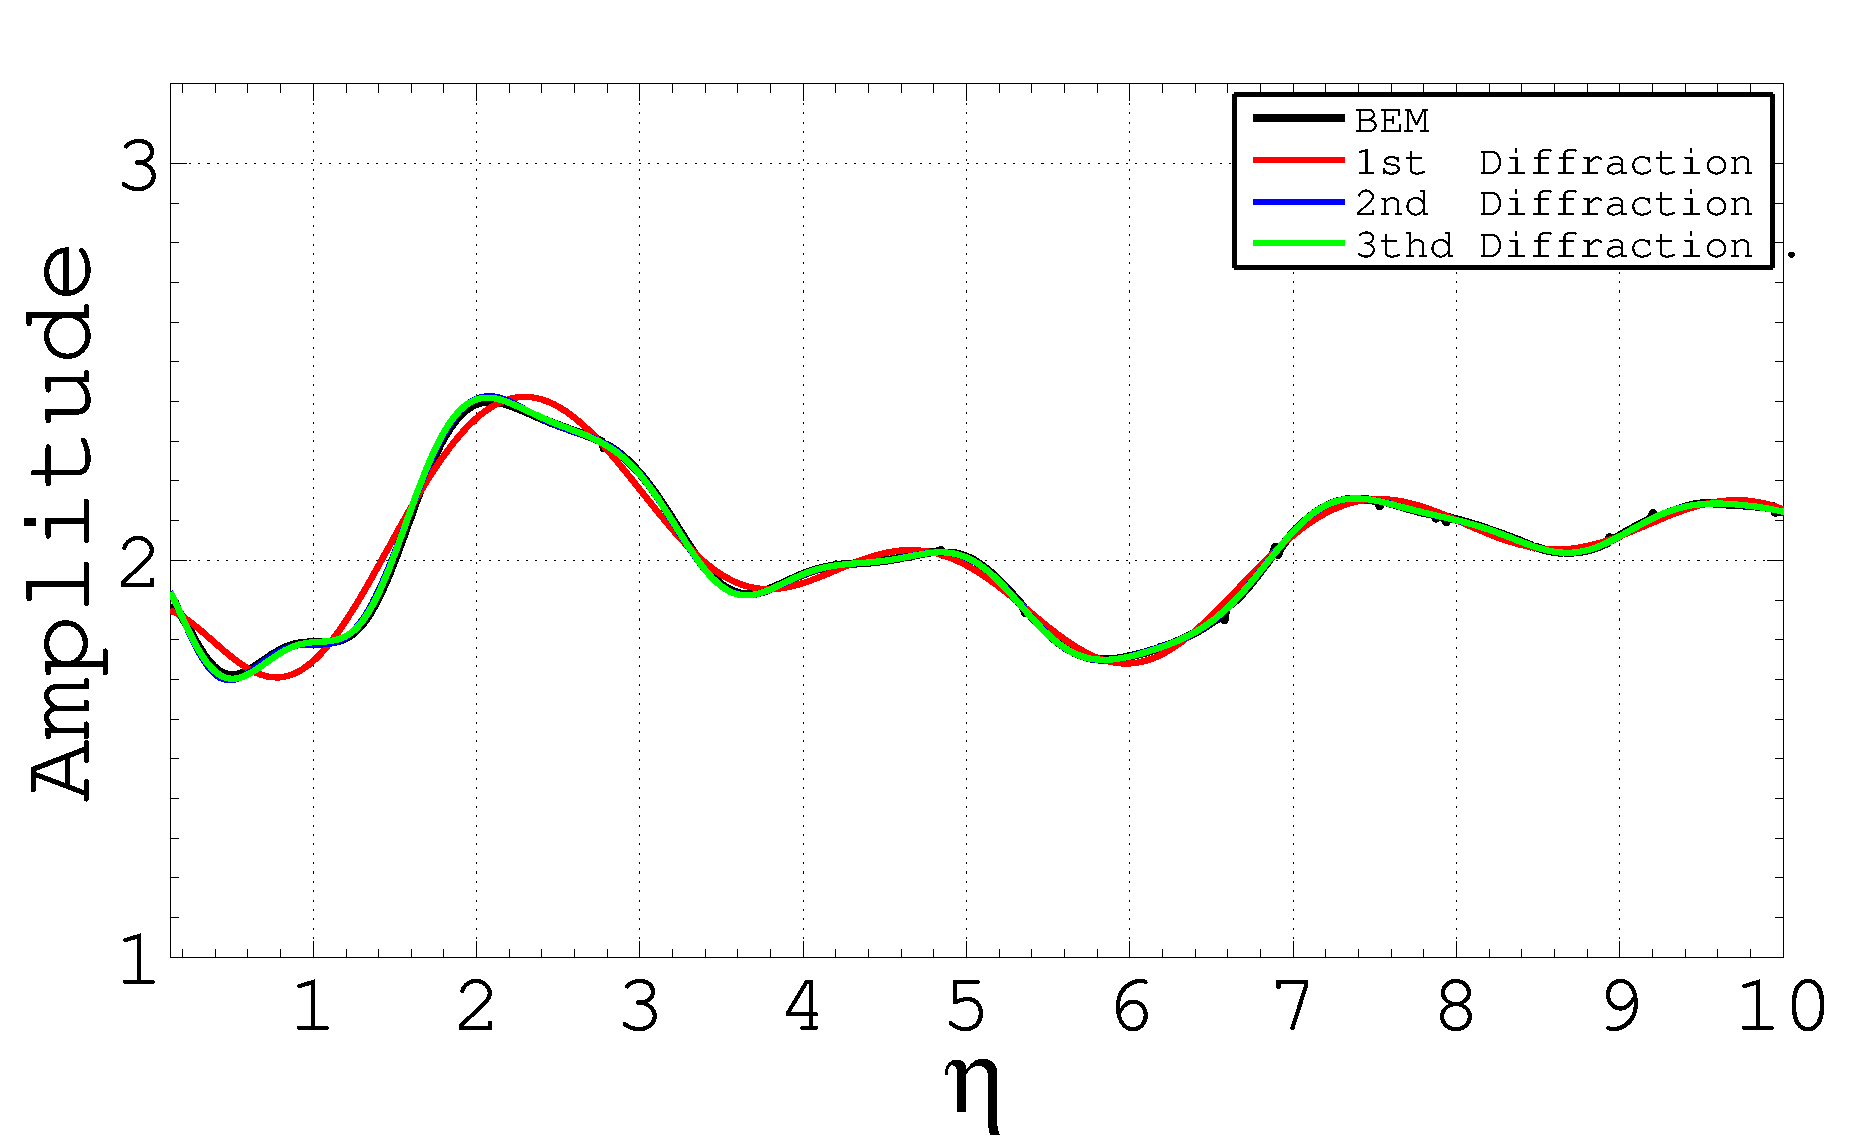
\includegraphics[width=4.0cm]{IMAGES/point1.pdf}}
		& \subfloat[BEM]{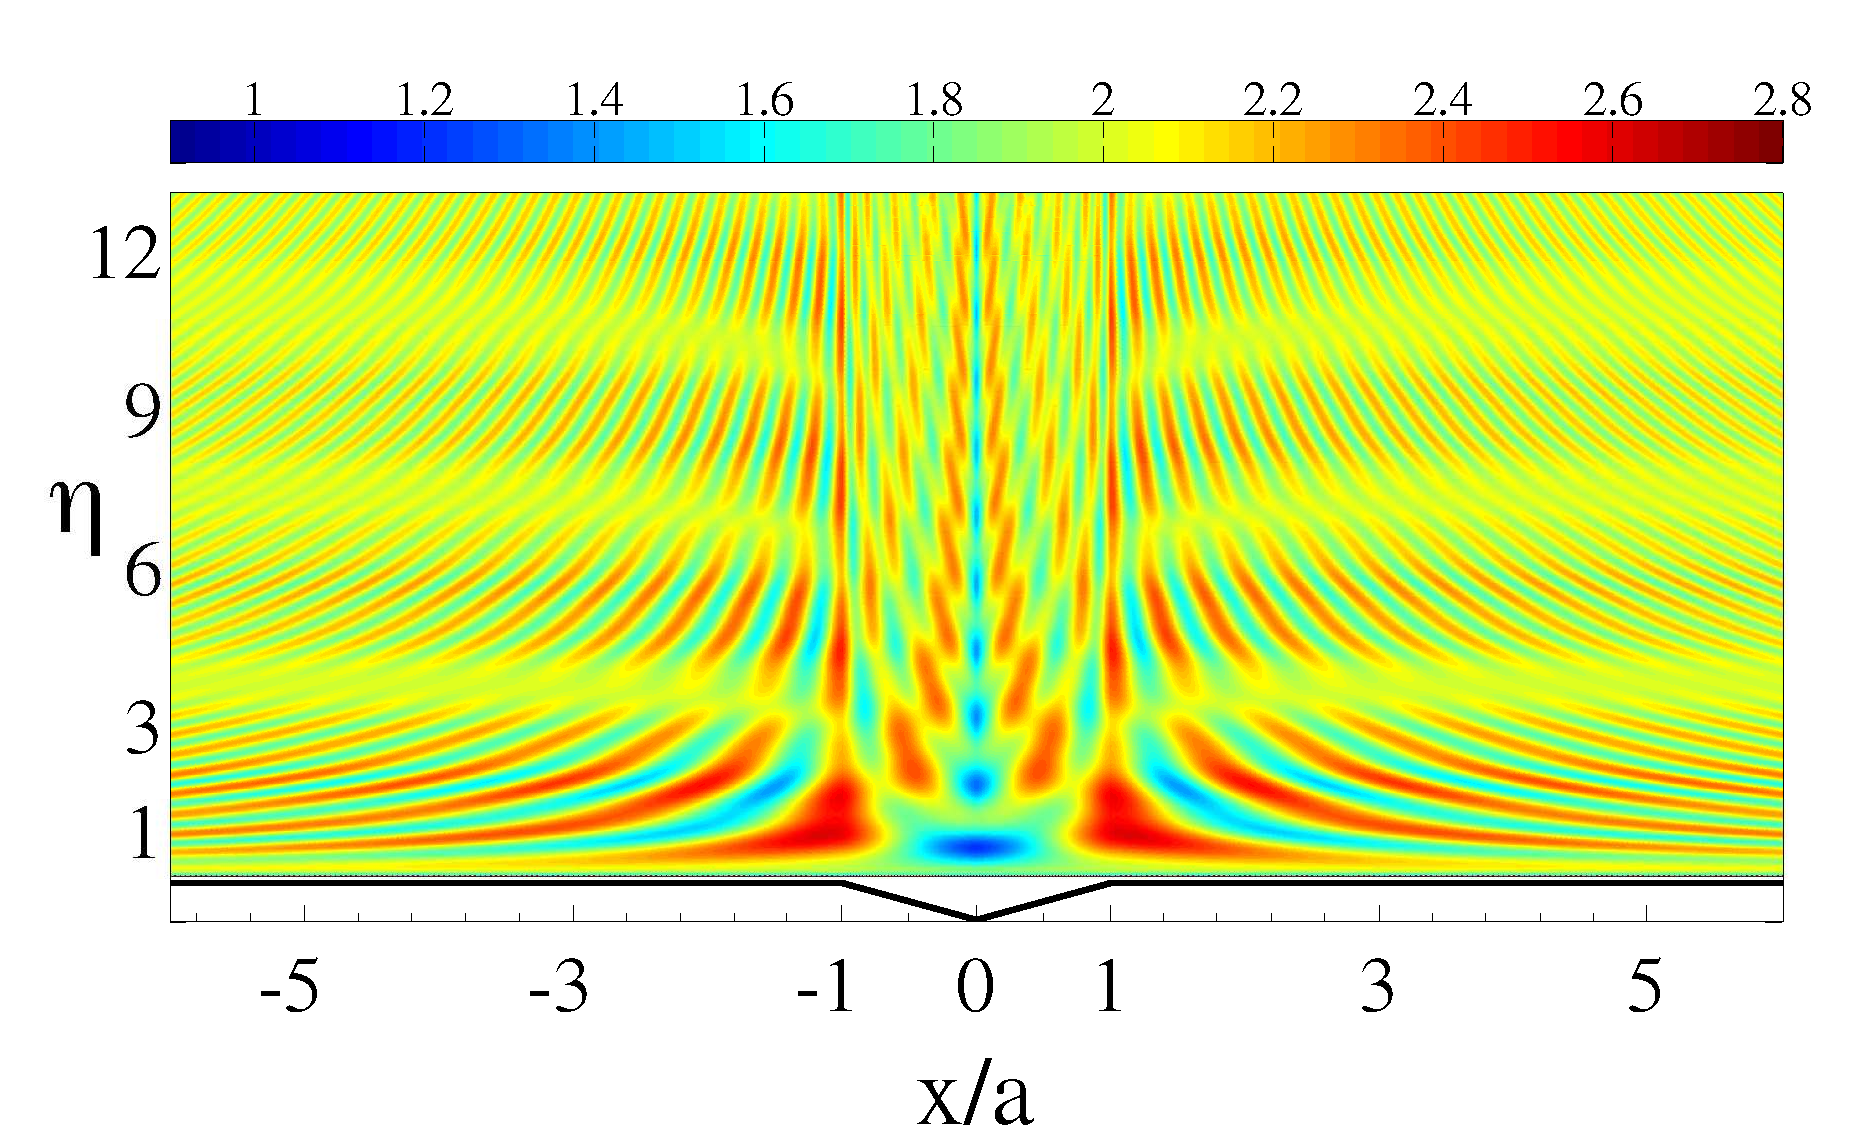
\includegraphics[width=4.0cm]{IMAGES/Completo.pdf}}
		& \subfloat[$\eta = 0.50$]{\includegraphics[width=4.0cm]{IMAGES/fts50.pdf}}
   		& \subfloat[$\eta = 2.50$]{\includegraphics[width=4.0cm]{IMAGES/fts250.pdf}}
   		%
   		\vspace{-0.4 cm}	
   		& \subfloat[$x/a=1.50$]{\includegraphics[width=4.0cm]{IMAGES/point2.pdf}}
		& \subfloat[1st Order Diffraction]{\includegraphics[width=4.0cm]{IMAGES/Diffracted1.pdf}}
		& \subfloat[$\eta = 1.00$]{\includegraphics[width=4.0cm]{IMAGES/fts100.pdf}}
   		& \subfloat[$\eta = 3.00$]{\includegraphics[width=4.0cm]{IMAGES/fts300.pdf}}
   		%
   		\vspace{-0.4 cm}
   		& \subfloat[$x/a=2.50$]{\includegraphics[width=4.0cm]{IMAGES/point3.pdf}}
   		& \subfloat[2nd Order Diffraction]{\includegraphics[width=4.0cm]{IMAGES/Diffracted2.pdf}}
		& \subfloat[$\eta = 1.50$]{\includegraphics[width=4.0cm]{IMAGES/fts150.pdf}}
   		& \subfloat[$\eta = 3.50$]{\includegraphics[width=4.0cm]{IMAGES/fts350.pdf}}
   		%
   		\vspace{-0.4 cm}
   		& \subfloat[$x/a=3.50$]{\includegraphics[width=4.0cm]{IMAGES/point4.pdf}}
		& \subfloat[3thd Order Diffraction]{\includegraphics[width=4.0cm]{IMAGES/Diffracted3.pdf}}
		& \subfloat[$\eta = 2.00$]{\includegraphics[width=4.0cm]{IMAGES/fts200.pdf}}
   		& \subfloat[$\eta = 4.00$]{\includegraphics[width=4.0cm]{IMAGES/fts400.pdf}}
   		
	\end{tabular}
%
%\end{tabularx}
\caption{Frequency domain response for the $V$-shaped canyon topography. Column 2 displays frequency-space contour maps for the spatial distribution of the amplitude of the transfer function obtained with a BEM algorithm and with the current SBD technique with up to 3 orders of diffraction. Column 1 shows the amplitude functions at constant locations for different recievers over the canyon surface while columns 3 and 4 display the amplitude function for constant dimensionless frequencies and for receiver over the free surface.}\label{fig:jaja}
\end{figure}
\end{landscape}

\begin{figure}[H]
	\centering
	\subfloat[BEM/SBD-first-O.D]{\includegraphics[width=5.5cm]{IMAGES/Factor1.pdf}}\
	\hspace{-.5cm}
	\subfloat[SBD-first-O.D/SBD-third-O.D]{\includegraphics[width=5.5cm]{IMAGES/Factor13.pdf}}\\
	\subfloat[BEM/SBD-second-O.D]{\includegraphics[width=5.5cm]{IMAGES/Factor2.pdf}}\
	\hspace{-.5cm}
	\subfloat[SBD-first-O.D/SBD-second-O.D]{\includegraphics[width=5.5cm]{IMAGES/Factor12.pdf}}\\
	\subfloat[BEM/SBD-third-O.D]{\includegraphics[width=5.5cm]{IMAGES/Factor3.pdf}}\
	\hspace{-.5cm}
	\subfloat[SBD-second-O.D/SBD-third-O.D]{\includegraphics[width=5.5cm]{IMAGES/Factor23.pdf}}
	\caption{Contour maps for the BEM to SBD ratios for different orders of diffraction (column 1) and ratios between the SBD results with different orders of diffraction (column 2).}
	\label{fig:difrac}
\end{figure}
%
The computations with the SBD approach, which were progressively obtained with $1$, $2$ and $3$ orders of diffraction and error measures defined like $\mid BEM - SBD \mid / \mid BEM \mid$ were computed for each solution. \Cref{fig:errorfrec} displays the error for receivers over the free surface and measured with respect to the BEM response considering up to 3 orders of diffraction. In computing the error we considered a range of frequencies from $\eta=0.0625$ to $\eta=15.0$. A large difference between the SBD solution with only 1 diffraction order and those with 2 and 3 orders is clearly observed. This is due to the secondary reflections experienced by the first diffracted waves over the free surface of the half-space where its amplitude is doubled. The above error measure is also shown in \cref{fig:errorrealcomplex} for the real and imaginary component of the response.
%
\begin{figure}[H]
	\centering
	\includegraphics[width=10cm]{IMAGES/Error_Frequency_Domain.pdf}
	\caption{Error in the total field obtained in the frequency domain with 1, 2 and 3 orders of diffraction.
	\label{fig:errorfrec}}
\end{figure}
%
\begin{figure}[H]
	\centering
	\subfloat[Error for the real component of the transfer function]{\includegraphics[width=6.0cm]{IMAGES/Error_Real.pdf}}\
	\hspace{-.1cm}
	\subfloat[Error for the imaginary component of the transfer function]{\includegraphics[width=6.0cm]{IMAGES/Error_Complex.pdf}}\\
	\caption{Error measures for the real and imaginary parts of the transfer function obtained with the BEM and the SBD methods .}
	\label{fig:errorrealcomplex}
\end{figure}
%
\Cref{fig:sabanascontor} displays synthetic seismograms for receivers over the canyon surface computed with the BEM algorithm and with the SBD technique using 1, 2 and 3 orders of diffraction. A qualitative comparisson of these results shows how the only difference between the two sets appears in a diffracted front emanating from the inferior wedge. This front is missing from the synthetics corresponding to a single diffraction term. Such discontinuity is not present in the synthetics for 2 and 3 diffraction orders since it corresponds to a second order diffraction that originates when the main diffracted front from the upper wedge interacts with the inferior wedges from the canyon. In this case the second order diffracted field, experiences an additional diffraction event producing a third order front that travels almost in-phase with the second order front. These fronts separate from each other as the distance from the scatterer increases.
%
\begin{figure}[H]
	\centering
	\subfloat[BEM]{\includegraphics[width=6.0cm]{IMAGES/sabana_bem.pdf}}\
	\hspace{-.25cm}
	\subfloat[SBD-first-O.D]{\includegraphics[width=6.0cm]{IMAGES/sabana_dif1.pdf}}\\
	\vspace{-1.5cm}
	\subfloat[SBD-second-O.D]{\includegraphics[width=6.0cm]{IMAGES/sabana_dif2.pdf}}\,
	\hspace{-.25cm}
	\subfloat[SBD-third-O.D]{\includegraphics[width=6.0cm]{IMAGES/sabana_dif3.pdf}}
	\vspace{-.25cm}
	\caption{Synthetic seismograms for receivers over the canyon surface obtained with the BEM algorithm and the current SBD approach.}
	\label{fig:sabanascontor}
\end{figure}
%
\Cref{fig:historypoints} shows synthetic seismograms computed with the BEM algorithm and with the SBD technique using 1,2 and 3 orders of diffraction at 4 different locations. It is observed, once again, how the time domain response is recovered almost completely by considering only diffraction effects up to third order. The contribution from higher order terms has an amplitude which is already very small with respect to the amplitude from the incident field. Moreover, these higher order diffraction effects are highly delayed with respect to the incident field. This is also verified by the error measures shown in \cref{fig:errortime} corresponding to receivers over the free surface and calculated with respect to the numerical BEM solution. This field is compared with the results obtained from the SBD technique for 1, 2 and 3 orders of diffraction. Clearly, the smaller error occurs for the solution with third diffraction order effects. It must be realized that in the time domain the magnitude of the incident field is highly important since large amplitudes imply that diffracted fields required large distances to vanish.
%
\begin{figure}[H]
	\centering
	\subfloat[History at $x/a=0.50$]{\includegraphics[width=6.0cm]{IMAGES/History_point_1.pdf}}\
	\hspace{-.25cm}
	\subfloat[History at $x/a=1.50$]{\includegraphics[width=6.0cm]{IMAGES/History_point_2.pdf}}\\
	\vspace{-1.5cm}
	\subfloat[History at $x/a=2.00$]{\includegraphics[width=6.0cm]{IMAGES/History_point_3.pdf}}\,
	\hspace{-.25cm}
	\subfloat[History at $x/a=2.50$]{\includegraphics[width=6.0cm]{IMAGES/History_point_4.pdf}}
	\vspace{-.25cm}
	\caption{Synthetic seismograms at selected receivers over the canyon surface obtained with the BEM algorithm and the current SBD approach..}
	\label{fig:historypoints}
\end{figure}
%
\begin{figure}[H]
	\centering
	\includegraphics[width=10cm]{IMAGES/Error_Time_Domain.pdf}
	\caption{Total field error related to the time domain results obtained with the BEM and the SBD technique with 1, 2 and 3 orders of diffraction. 
\label{fig:errortime}}
\end{figure}


\subsection*{Conclusions}
\phantomsection
\addcontentsline{toc}{subsection}{Conclusions}

We have proposed a method to determine the frequency domain solution to the problem of scattering of horizontally polarized shear waves in a homogeneous half-space with a general surface irregularity resembling a topographic effect. The method of analysis is based on the representation of the surface geometry by a superposition of wedges. The solution is then obtained after adding to the optical field the diffracted waves required to obtain a total continuous field and produced by the corner singularity of the different wedges. Since the conceptual basis if the method is the addition of diffracted waves the technique has been named superposition based diffraction. Although the process of building a solution may become tedious for complex geometries, it serves as a conceptual tool for the analysis of numerical solutions and also for the case of in-plane waves.



%%%%%%%%%%%%%%%%%%%%%%%%%%%%%%%%%%%%%%%%%%%%%%%%%%%%%%%%%%%%%%%%%%%%%%%
%%%% %%%%%%%%%%%%%%%%%%%%%%%%R E S O L U C I O N%%%%%%%%%%%%%%%%%%%%%%%%%%%%%%%
%%%%%%%%%%%%%%%%%%%%%%%%%%%%%%%%%%%%%%%%%%%%%%%%%%%%%%%%%%%%%%%%%%%%%%%
\newpage

\section{Topographic resolution: towards a rational approach for geometric effects}
\phantomsection
\addcontentsline{toc}{section}{Topographic resolution}

The exponential increase in computer power together with the continuing development in robust numerical algorithms has facilitated the creation of highly realistic seismic scenarios including source-path effects and geometrically complex propagation media (Add references). These numerical models are useful as they accurately provide a high resolution description of the ground response at a specific region and for a particular earthquake motion, thus helping identify particular propagation patterns and motion variations at specific locations. Paradoxically, the results from these highly realistic simulations are difficult to interpret and despite predicting the exact response at a site, the most interesting physically-based conclusions can only be drawn in very broad terms. At the other end, theoretical models based upon strong idealizations, and certainly fundamental in providing physical insight into the problem, also turn out to be very limited for realistic applications. Due to the presence of an apparently large number of geometric and mechanic parameters in the problem of site effects, the vast majority of code-based approaches still rely on 1D propagation models completely neglecting 3D and 2D effects.

The current work tackles the problem of ground response estimation in complex geometric scenarios from an engineering and practical perspective (e.g., with a limited quality of field data), but recognizing the increased presence within modern consulting companies of computing resources in terms of hardware, software and engineering personal. Concretely, this work focuses in the construction of numerical models, but in contrast to the goal of large scale computational simulations, which attempt to predict the exact response, the current proposal provides guidelines on how to construct simplified versions with limited prediction capabilities. In general our main objective here is to produce a rational simplification of the complete topography dictated by the analysis requirements. Specifically, in order to establish an objective level of model simplification, a target analysis frequency is prescribed which is typically connected to the lower structural period expected at the site. The result is an on-demand method that will produce a model simplified enough to predict ground motions valid up to a given range of structural periods. The simplified model would then include only those topographic details required for an accurate prediction of the response up to the specified target frequency. 

The proposed method builds upon the fundamental  physical aspects of the diffraction based approach described previously, and more specifically on the understanding that a topographic irregularity corresponds to a superposition of wedges (introducing sources of diffraction). The wedge emerges then as the basic geometric element controlling the response. By analogy with the required size of a discrete element in a numerical method which depends on the analysis frequency, here a wedge-frequency relation determines the resolution of the model: accordingly, this work introduces the concept of topographic resolution. A characteristic dimension is provided to the wedge, after noticing that actual topography is not necessarily conformed by sharp irregularities but by surfaces with a given degree of smoothness. This means that a topographic irregularity can be equivalently modeled by a singular wedge or by a smooth curve tangent to the wedge. This approximation immediately introduces as the characteristic wedge dimension the distance between the smooth-curve tangent to the wedge and its corner singularity. 


In this section we study the connection between the topographic resolution in terms of the minimum wedge dimension present in the model and the expected frequency content of the response. These new concepts are explored in the analysis of canonical surface topographies. The main purpose through this rational and systematic approach is to identify the topographic features that are effectively relevant to capture motion aggravation for a specific range of target periods. 

\subsection*{Topographic resolution}
\addcontentsline{toc}{subsection}{Topographic resolution}
This section introduces the idea of topographic element defined as the fundamental building block in terms of which it is possible to construct a surface irregularity of arbitrary shape. Its characteristic dimension $h_{top}$ can be connected to the wavelength of the incident field by the dimensionless frequency parameter:

\begin{equation}
\eta  = \frac{{{h_{top}}}}{{{\lambda ^{\min }}}}.
\label{Eq:topogra}
\end{equation}

\Cref{Eq:topogra} is analogous to the relation between wavelength $\lambda$ and the characteristic element size $h_{num}$ in a numerical discretization intended for wave propagation analysis where the dimensionless frequency parameter

\begin{equation}
\alpha  = \frac{{{h_{num}}}}{{{\lambda ^{\min }}}},
\label{Eq:numerical}
\end{equation}

is indicative of the number of elements per minimum wavelength. In wave propagation analysis conducted with the finite element method a common criteria is to use $\alpha = 0.1$ (or equivalently $10$ elements per wavelength). In the above $\lambda^{min} = \beta / f_{max}$ and $f_{max}$ is the maximum frequency of the incident field while $\beta$ is the wave propagation velocity in the media.

In the context of topographic or geometric effects $\eta$ plays the same role as $\alpha$ in \cref{Eq:numerical}, however it must be observed that here $\eta$ prescribes the number of wavelengths that fit into the topographic element with a high frequency field corresponding to a large value of $\eta$. Clearly the dimensionless frequency $\eta$ controls the topographic resolution of the actual topography in such a way that a prescribed value of $\eta$ indicates the quality of the model. In the construction of a model for topographic effects we are interested in identifying the minimum geometric features that must be included in order to capture the response up to a given target frequency. In this work the target frequency (or equivalently $\lambda^{tar}$) is connected to the range of structural periods for which the analysis is carried out in the first place. Hence we can write for the minimum value of the characteristic dimension of the topographic element:

\begin{equation}
h_{top}^{min} = \eta \lambda^{tar}.
\label{Eq:target}
\end{equation}

The parameter $h_{top}^{min}$ in \cref{Eq:target} indicates that all topographic irregularities with characteristic dimension $\ell $ smaller than $h_{top}^{min}$ are unnecessary if the analysis is expected to predict accurate results up to the target frequency  $f^{tar} = \beta / {\lambda ^{tar }}$. Alternatively, $h_{top}^{min}$, indicates which irregularities of the topographic profile are relevant for the specific range of structural periods for which the analysis is being conducted. This idea is illustrated in \cref{fig:part_spec} where we schematize a response spectra resulting from an analysis with irregularities smaller than $h_{top}^{min}$ being removed. The spectra is valid only for periods larger than ${T_{tar}}$ as shown by the shaded area.


\begin{figure}[H]
	\centering
	\subfloat{\includegraphics[width=7cm]{images/spec_prelim.png}}
	\caption{\small Topography dependent response spectra. The target structural period ${T_{tar}}$ sets the size of the minimum topographic element that must be retained in the analysis in order to predict results accurate only in a limited period range.} 
	\label{fig:part_spec}
\end{figure}


\subsection*{Building block in the construction of a topographic irregularity}
\addcontentsline{toc}{subsection}{Building block in the construction of a topographic irregularity}

As shown previously, a surface irregularity of arbitrary shape can be built through the superposition of several wedges making evident the fact that the fundamental topographic element or basic shape for the construction of very general topographic profiles is precisely the infinite wedge. This approach of building analytic solutions for general geometries under incident $SH$ waves is detailed in \cite{Jaramillo2012Analytic} and \cite{Gomez2016superposition}. To clarify further, two of such fundamental building blocks, or in what follows topographic elements, are shown in \cref{fig:approch} for a convex and concave geometry respectively. This fundamental wedge is described by its angle $\theta$ and by a corner singularity (or source of diffraction) $D$. Notice that this fundamental wedge does not have a characteristic element size as required by \cref{Eq:target}. However a characteristic dimension can be introduced after noticing the fact that an actual topographic irregularity has a shape which is closer represented by a smooth surface rather than by a singular wedge. A particular smooth approximation is shown in red line in \cref{fig:approch}.The curve, denoted like $C$ is tangent to the wedge at points $P_1$ and $P_2$ and it is at a distance $d$ from the wedge $D$. If we now simultaneously represent a topographic profile with a singular wedge $D$ and with a tangent curve $C$ and the differences in the response from both models are negligible, then all the topographic irregularities of dimension smaller than $d$ are irrelevant for the actual incident field. Therefore $d$ is the characteristic dimension of the topographic element defined in \cref{Eq:target} and giving the required level of topographic resolution.

\begin{figure}[H]
	\centering
	\subfloat{\includegraphics[width=10cm]{images/base.png}}
	\caption{\small Building block to be used in the approximate representation of topographical features of general shape. The actual surface may resemble the singular wedge (blue line) or the continuous tangent curve (red line). The separation distance $d$ controls the differences in the response in each wedge, however up to a certain value of this resolution parameter $d$ both solutions are considered to be equivalent implying that topographic features of dimension smaller than $d$ are irrelevant for the model.} 
	\label{fig:approch}
\end{figure}


An objective value for the size of the topographic element for a prescribed target period is obtained on the basis of the normalized square root of the squared difference between the amplitude of the transfer function computed with the singular wedge $D$ and a valid tangent approximation $C$. This error measure is defined like:


 \begin{equation}
 	\begin{split}
 		\delta & =  \sqrt{ \dfrac{1}{n} \sum_{i=1}^{n}(FT_{s_i} - FT_{c_i})^2}.\\
		\label{eq:quality}
 	\end{split}
 \end{equation}
 
where $FT_{s_i} =$ amplitude of the transfer function obtained from the singular wedge approximation; $FT_{c_i} =$ amplitude of the transfer function obtained from the curved approximation; and $n =$ number of observation points along the free surface of the wedge.

\Cref{fig:wedge} shows the variation of the error measure $\delta$ vs dimensionless frequency $\eta$ along the wedge for different values of the wedge angle $\theta$ and topographic element size $d$. An acceptable limit value of $\delta = 0.10$ is indicated by the dashed green line which intercepts the plot at the maximum dimensionless frequency $\eta_{max}$. This is the maximum value of the dimensionless frequency for which both models predict equivalent results. Hence for a specified value of the target frequency the corresponding value of  $\eta_{max}$ can be used to find the required topographic resolution $d$.


\begin{figure}[H]
	\centering
	\subfloat{\includegraphics[width=6cm]{images/etawedge.png}} 
	\caption{\small Variation of the error measure $\delta$ vs dimensionless frequency $\eta$ for different values of the wedge angle $\theta$ and topographic element size $d$. The dashed green line corresponds to the limit value of $\delta = 0.1$ and it intercepts the plot at $\eta_{max}$.} 
	\label{fig:wedge}
\end{figure}

As described in \cite{Jaramillo2012Analytic} in the context  of $SH$ waves, the spatial variability in the response due to surface topography is a function of the number of sources of diffraction and its separation distance. The interaction between sources is expected to be stronger at shorter separation distances. From the above it can be concluded that if one uses the idea of a topographic element as the fundamental geometric entity controlling the response of a topographic irregularity, this response is a function of the size $D$ of the different topographic element and its separation distances. This idea is explained further in \cref{fig:superpo} which shows the superposition of two topographic elements where the additional parameter $L_W$ corresponds to the distance between points $P_1$ and $P_2$ in adjacent elements. This parameter can be defined in terms of the target frequency and the characteristic size of the topographic element as:

\begin{equation}
\begin{split}
L_W= Nd = N  \eta {\lambda ^ {tar}}   \\
\label{Eq:dist}
\end{split}
\end{equation}

where $N$ is an integer factor that can be understood as a dimensionless distance between wedges.

\begin{figure}[H]
	\centering
	\subfloat{\includegraphics[width=10cm]{images/dist.png}}
	\caption{\small Topographic irregularity conformed by two hills and a canyon and resulting from the superposition of fundamental building blocks. In this schematic description the hills have been assumed as singular wedges (blue lines) while the canyon has been approximated by the continuous wedge (red line).} 
	\label{fig:superpo}
\end{figure}


\subsection*{Response of canonical topographies}
\addcontentsline{toc}{subsection}{Response of canonical topographies}

After emphasizing the fact that the geometric parameters $d$ and $L_W$ (or its dimensionless counterparts $\eta$ and $N$) completely describe the topographic element, it is necessary to study its influence in the response. We do this in terms of a parametric analysis of canonical topographies corresponding to a trapezoidal and a V-shaped canyon and a trapezoidal and a V-shaped hill. These shapes can be easily constructed from superposition of several topographic elements. As shown in \cref{fig:canonicos1} and \cref{fig:canonicos2}  each shape is defined by its slope angle $\alpha$ and by the geometric parameters $d$ and $L_W$ defining the conforming topographic elements. Notice that the main geometric difference between the V-shaped canyon and the trapezoidal canyon is the existence of the horizontal length of extension $L_W$ at the bottom of the latter which allows the diffracted waves generated at the singularities to dissipate with distance.

\begin{figure}[H]
\centering
\includegraphics[width=8.5cm]{images/canonics.png}
\caption{\small Canonic forms corresponding to a trapezoidal and a V-shaped canyon used in the calibration of the error parameter $\delta$. The frequency domain response using the singular wedge approximation (blue line) and the tangent curve approximation (red line) under vertically incident $SH$ and $SV$ waves was computed with an in-house implementation of the direct boundary element method.}
\label{fig:canonicos1}
\end{figure}

\begin{figure}[H]
\centering
\includegraphics[width=8.5cm]{images/canonics2.png}
\caption{\small Canonic forms corresponding to a trapezoidal and a V-shaped hill used in the calibration of the error parameter $\delta$. The frequency domain response using the singular wedge approximation (blue line) and the tangent curve approximation (red line) under vertically incident $SH$ and $SV$ waves was computed with an in-house implementation of the direct boundary element method.}
\label{fig:canonicos2}
\end{figure}


As part of the parametric analysis the frequency domain response of each canonical topography under vertically incident $SH$ and $SV$ plane waves was computed with an in-house implementation of the direct boundary element method (add references). We studied canyons with slope angles $\alpha$ corresponding to $[20^\circ , 30^\circ , 40^\circ ]$, dimensionless separation distances $N$ of $[1 , 25 , 50]$ and varied the dimensionless frequency $\eta$ in the range $ [0.05, 10.0 ]$. In the parametric analysis each given shape (say V-shaped canyon with $\theta = 20^\circ$) is modeled by the complete singular wedge approximation and by several smooth representations corresponding to values of $N$ in the range $[1 , 25 , 50]$ and values of  $\eta$ in the range $ [0.05, 10.0 ]$ and in each resulting analysis we recorded the value of the error parameter $\delta$ as per \cref{eq:quality}. For each canonical shape we plotted the variation of $\delta$ with the dimensionless frequency $\eta$. A typical $\delta$ vs $\eta$ plot corresponding to $\alpha = 20.0 ^ \circ$ and $N = 1$ in the V-shaped canyon under incident $SH$ waves is shown in \cref{fig:trendsh}. In this plot the horizontal dashed green line marks the acceptable limit value of $\delta = 0.1$ while the value of $\eta$ corresponding to the point enclosed by the circle gives an upper bound in the dimensionless frequency range for which appropriate solutions can be obtained with a simplified model.


\begin{figure}[H]
	\centering
	\subfloat{\includegraphics[width=8cm]{{images/Results/delta_dL1_VSH20.pdf}}}
	\caption{\small Variation in the error measure $\delta$ vs dimensionless frequency $\eta$ in the V-shaped canyon under incident $SH$ waves for $\alpha = 20.0 ^ \circ$ and $L_W = 1$. For frequencies below $\eta = 2.0$ the results from both models are assumed equivalent.} 
	\label{fig:trendsh}
\end{figure}


To illustrate our approach we display in \cref{fig:FTVSHadd} a comparison of the spatial distribution of the amplitude function along the free surface of the V-shaped canyon under vertically incident $SH$ waves. In the figure each column corresponds to a different value of the slope angle $\alpha$, while each row represents a different value of the separation distance parameter $N$. The results are displayed for the maximum value of the dimensionless frequency taken from \cref{fig:trendsh}. 


\begin{figure}[H]
	\centering
	\subfloat{\includegraphics[scale=0.50]{images/Results/FT_VSH20_L1_20.pdf}\label{fig:FTVSH1}}
	\subfloat{\includegraphics[scale=0.50]{images/Results/FT_VSH30_L1_40.pdf}\label{fig:FTVSH2}}
	\subfloat{\includegraphics[scale=0.50]{images/Results/FT_VSH40_L1_50.pdf}\label{fig:FTVSH3}} \\
	\subfloat{\includegraphics[scale=0.50]{images/Results/FT_VSH20_L25_25.pdf}\label{fig:FTVSH4}}
	\subfloat{\includegraphics[scale=0.50]{images/Results/FT_VSH30_L25_40.pdf}\label{fig:FTVSH5}}
	\subfloat{\includegraphics[scale=0.50]{images/Results/FT_VSH40_L25_45.pdf}\label{fig:FTVSH6}} \\
	\subfloat{\includegraphics[scale=0.50]{images/Results/FT_VSH20_L50_30.pdf}\label{fig:FTVSH7}}
	\subfloat{\includegraphics[scale=0.50]{images/Results/FT_VSH30_L50_35.pdf}\label{fig:FTVSH8}}
	\subfloat{\includegraphics[scale=0.50]{images/Results/FT_VSH40_L50_50.pdf}\label{fig:FTVSH9}} \\
	\caption{Spatial variation of the amplitude of the transfer function along points of the surface of a V-shaped canyon when $SH$ waves is used. $N =1$, $25$ and  $50$; $\alpha=$ $20 \grad$, $30 \grad$ and $40 \grad$. blue line: straight approximation, black line: curve approximation}
	\label{fig:FTVSHadd}
\end{figure}



The complete set of results for the canonical topographies is shown in \cref{fig:TrendVSH} through \cref{fig:TrendTSV}. Similarly \cref{fig:FTtrapSV} through \cref{fig:FTVSH} compares the spatial distribution of the amplitude of the transfer function obtained with a model built from singular wedges and from the tangent curve approximation corresponding to the maximum admissible value of $\eta$ as per \cref{fig:TrendVSH} through \cref{fig:TrendTSV}. It is evident that as long as $\eta$ remains below the maximum admissible value the frequency domain response computed from both models remains unmodified.



%%%%%%%%%%
\begin{landscape}
\begin{figure}
\captionsetup[subfigure]{labelformat=empty}
\def\tabularxcolumn#1{m{#1}}
%\begin{tabularx}{\linewidth}{@{}Xc@{}}
%
%\subfloat[BEM]{\includegraphics[width=0.7\linewidth]{IMAGES/Completo.pdf}}
%
	\begin{tabular}{cccc}
		\subfloat{\includegraphics[width=7.0cm]{images/Results/delta_dL1_VSH20.pdf}}
%		\hspace{-1.5cm}
		& \subfloat{\includegraphics[width=7.0cm]{images/Results/delta_dL25_VSH20.pdf}}
%		\hspace{-1.5cm}
		& \subfloat{\includegraphics[width=7.0cm]{images/Results/delta_dL50_VSH20.pdf}}\\
%		\vspace{-1 cm}\\
		
		\subfloat{\includegraphics[width=7.0cm]{images/Results/delta_dL1_VSH30.pdf}}
%		\hspace{-1.5cm}
		& \subfloat{\includegraphics[width=7.0cm]{images/Results/delta_dL25_VSH30.pdf}}
%		\hspace{-1.5cm}
		& \subfloat{\includegraphics[width=7.0cm]{images/Results/delta_dL50_VSH30.pdf}}\\
%		\vspace{-1 cm}\\
		
		\subfloat{\includegraphics[width=7.0cm]{images/Results/delta_dL1_VSH40.pdf}}
%		\hspace{-1.5cm}
		& \subfloat{\includegraphics[width=7.0cm]{images/Results/delta_dL25_VSH40.pdf}}
%		\hspace{-1.5cm}
		& \subfloat{\includegraphics[width=7.0cm]{images/Results/delta_dL50_VSH40.pdf}}\\
%		\vspace{-1 cm}\\
   		
	\end{tabular}
%tsaur2008analytical
%\end{tabularx}
\caption{Trend of the $\delta$ criterion obtained in V-shaped canyon  when a angle $\alpha$ and $LD$ are set and the $SH$ waves is used . $Ld =1$, $25$ and  $50$; $\alpha=$ $20$\grad, $30$\grad and $40$\grad..}\label{fig:TrendVSH}
\end{figure}
\end{landscape}

\begin{landscape}
\begin{figure}
\captionsetup[subfigure]{labelformat=empty}
\def\tabularxcolumn#1{m{#1}}
%\begin{tabularx}{\linewidth}{@{}Xc@{}}
%
%\subfloat[BEM]{\includegraphics[width=0.7\linewidth]{IMAGES/Completo.pdf}}
%
	\begin{tabular}{cccc}
		\subfloat{\includegraphics[width=7.0cm]{images/Results/delta_dL1_VSV20.pdf}}
%		\hspace{-1.5cm}
		& \subfloat{\includegraphics[width=7.0cm]{images/Results/delta_dL25_VSV20.pdf}}
%		\hspace{-1.5cm}
		& \subfloat{\includegraphics[width=7.0cm]{images/Results/delta_dL50_VSV20.pdf}}\\
%		\vspace{-1 cm}\\
		
		\subfloat{\includegraphics[width=7.0cm]{images/Results/delta_dL1_VSV30.pdf}}
%		\hspace{-1.5cm}
		& \subfloat{\includegraphics[width=7.0cm]{images/Results/delta_dL25_VSV30.pdf}}
%		\hspace{-1.5cm}
		& \subfloat{\includegraphics[width=7.0cm]{images/Results/delta_dL50_VSV30.pdf}}\\
%		\vspace{-1 cm}\\
		
		\subfloat{\includegraphics[width=7.0cm]{images/Results/delta_dL1_VSV40.pdf}}
%		\hspace{-1.5cm}
		& \subfloat{\includegraphics[width=7.0cm]{images/Results/delta_dL25_VSV40.pdf}}
%		\hspace{-1.5cm}
		& \subfloat{\includegraphics[width=7.0cm]{images/Results/delta_dL50_VSV40.pdf}}\\
%		\vspace{-1 cm}\\
   		
	\end{tabular}
%tsaur2008analytical
%\end{tabularx}
\caption{Trend of the $\delta$ criterion obtained in V-shaped canyon  when a angle $\alpha$ and $LD$ are set and the $SV$ waves is used . $Ld =1$, $25$ and  $50$; $\alpha=$ $20$\grad, $30$\grad and $40$\grad..}\label{fig:TrendVSV}
\end{figure}
\end{landscape}

\begin{landscape}
\begin{figure}
\captionsetup[subfigure]{labelformat=empty}
\def\tabularxcolumn#1{m{#1}}
%\begin{tabularx}{\linewidth}{@{}Xc@{}}
%
%\subfloat[BEM]{\includegraphics[width=0.7\linewidth]{IMAGES/Completo.pdf}}
%
	\begin{tabular}{cccc}
		\subfloat{\includegraphics[width=7.0cm]{images/Results/delta_dL1_TSH20.pdf}}
%		\hspace{-1.5cm}
		& \subfloat{\includegraphics[width=7.0cm]{images/Results/delta_dL25_TSH20.pdf}}
%		\hspace{-1.5cm}
		& \subfloat{\includegraphics[width=7.0cm]{images/Results/delta_dL50_TSH20.pdf}}\\
%		\vspace{-1 cm}\\
		
		\subfloat{\includegraphics[width=7.0cm]{images/Results/delta_dL1_TSH30.pdf}}
%		\hspace{-1.5cm}
		& \subfloat{\includegraphics[width=7.0cm]{images/Results/delta_dL25_TSH30.pdf}}
%		\hspace{-1.5cm}
		& \subfloat{\includegraphics[width=7.0cm]{images/Results/delta_dL50_TSH30.pdf}}\\
%		\vspace{-1 cm}\\
		
		\subfloat{\includegraphics[width=7.0cm]{images/Results/delta_dL1_TSH40.pdf}}
%		\hspace{-1.5cm}
		& \subfloat{\includegraphics[width=7.0cm]{images/Results/delta_dL25_TSH40.pdf}}
%		\hspace{-1.5cm}
		& \subfloat{\includegraphics[width=7.0cm]{images/Results/delta_dL50_TSH40.pdf}}\\
%		\vspace{-1 cm}\\
   		
	\end{tabular}
%tsaur2008analytical
%\end{tabularx}
\caption{Trend of the $\delta$ criterion obtained in Trapezoidal canyon  when a angle $\alpha$ and $LD$ are set and the $SH$ waves is used . $Ld =1$, $25$ and  $50$; $\alpha=$ $20$\grad, $30$\grad and $40$\grad.}\label{fig:TrendTSH}
\end{figure}
\end{landscape}

\begin{landscape}
\begin{figure}
\captionsetup[subfigure]{labelformat=empty}
\def\tabularxcolumn#1{m{#1}}
%\begin{tabularx}{\linewidth}{@{}Xc@{}}
%
%\subfloat[BEM]{\includegraphics[width=0.7\linewidth]{IMAGES/Completo.pdf}}
%
	\begin{tabular}{cccc}
		\subfloat{\includegraphics[width=7.0cm]{images/Results/delta_dL1_TSV20.pdf}}
%		\hspace{-1.5cm}
		& \subfloat{\includegraphics[width=7.0cm]{images/Results/delta_dL25_TSV20.pdf}}
%		\hspace{-1.5cm}
		& \subfloat{\includegraphics[width=7.0cm]{images/Results/delta_dL50_TSV20.pdf}}\\
%		\vspace{-1 cm}\\
		
		\subfloat{\includegraphics[width=7.0cm]{images/Results/delta_dL1_TSV30.pdf}}
%		\hspace{-1.5cm}
		& \subfloat{\includegraphics[width=7.0cm]{images/Results/delta_dL25_TSV30.pdf}}
%		\hspace{-1.5cm}
		& \subfloat{\includegraphics[width=7.0cm]{images/Results/delta_dL50_TSV30.pdf}}\\
%		\vspace{-1 cm}\\
		
		\subfloat{\includegraphics[width=7.0cm]{images/Results/delta_dL1_TSV40.pdf}}
%		\hspace{-1.5cm}
		& \subfloat{\includegraphics[width=7.0cm]{images/Results/delta_dL25_TSV40.pdf}}
%		\hspace{-1.5cm}
		& \subfloat{\includegraphics[width=7.0cm]{images/Results/delta_dL50_TSV40.pdf}}\\
%		\vspace{-1 cm}\\
   		
	\end{tabular}
%tsaur2008analytical
%\end{tabularx}
\caption{Trend of the $\delta$ criterion obtained in Trapezoidal canyon  when a angle $\alpha$ and $LD$ are set and the $SV$ waves is used . $Ld =1$, $25$ and  $50$; $\alpha=$ $20$\grad, $30$\grad and $40$\grad..}\label{fig:TrendTSV}
\end{figure}
\end{landscape}


%%%%%%%%%%%

\begin{landscape}
\begin{figure}
\captionsetup[subfigure]{labelformat=empty}
\def\tabularxcolumn#1{m{#1}}
%\begin{tabularx}{\linewidth}{@{}Xc@{}}
%
%\subfloat[BEM]{\includegraphics[width=0.7\linewidth]{IMAGES/Completo.pdf}}
%
	\begin{tabular}{cccc}
		\subfloat{\includegraphics[width=7.0cm]{images/Results/FT_VSH20_L1_20.pdf}}
%		\hspace{-1.5cm}
		& \subfloat{\includegraphics[width=7.0cm]{images/Results/FT_VSH30_L1_40.pdf}}
%		\hspace{-1.5cm}
		& \subfloat{\includegraphics[width=7.0cm]{images/Results/FT_VSH40_L1_50.pdf}}\\
%		\vspace{-1 cm}\\
		
		\subfloat{\includegraphics[width=7.0cm]{images/Results/FT_VSH20_L25_25.pdf}}
%		\hspace{-1.5cm}
		& \subfloat{\includegraphics[width=7.0cm]{images/Results/FT_VSH30_L25_40.pdf}}
%		\hspace{-1.5cm}
		& \subfloat{\includegraphics[width=7.0cm]{images/Results/FT_VSH40_L25_45.pdf}}\\
%		\vspace{-1 cm}\\
		
		\subfloat{\includegraphics[width=7.0cm]{images/Results/FT_VSH20_L50_30.pdf}}
%		\hspace{-1.5cm}
		& \subfloat{\includegraphics[width=7.0cm]{images/Results/FT_VSH30_L50_35.pdf}}
%		\hspace{-1.5cm}
		& \subfloat{\includegraphics[width=7.0cm]{images/Results/FT_VSH40_L50_50.pdf}}
%		\vspace{-1 cm}\\
   		
	\end{tabular}
%tsaur2008analytical
%\end{tabularx}
\caption{Spatial variation of the amplitude of the transfer function along surface points for a V-shaped canyon under incident $SH$ waves represented by singular wedges (blue line) and by tangent curves (black line) for values of the dimensionless distance  $N =1$, $25$ and  $50$ and canyon angles $\alpha$ in the range $[20^\circ , 30^\circ , 40^\circ ]$. The model with a tangent curve approximation corresponds to the maximum value of $\eta$ extracted from \cref{fig:TrendVSH} .}\label{fig:FTVSH}
\end{figure}
\end{landscape}


\begin{landscape}
\begin{figure}
\captionsetup[subfigure]{labelformat=empty}
\def\tabularxcolumn#1{m{#1}}
%\begin{tabularx}{\linewidth}{@{}Xc@{}}
%
%\subfloat[BEM]{\includegraphics[width=0.7\linewidth]{IMAGES/Completo.pdf}}
%
	\begin{tabular}{cccc}
		\subfloat{\includegraphics[width=7.0cm]{images/Results/FT_VSV20_L1_40.pdf}}
%		\hspace{-1.5cm}
		& \subfloat{\includegraphics[width=7.0cm]{images/Results/FT_VSV30_L1_40.pdf}}
%		\hspace{-1.5cm}
		& \subfloat{\includegraphics[width=7.0cm]{images/Results/FT_VSV40_L1_40.pdf}}\\
%		\vspace{-1 cm}\\
		
		\subfloat{\includegraphics[width=7.0cm]{images/Results/FT_VSV20_L25_30.pdf}}
%		\hspace{-1.5cm}
		& \subfloat{\includegraphics[width=7.0cm]{images/Results/FT_VSV30_L25_45.pdf}}
%		\hspace{-1.5cm}
		& \subfloat{\includegraphics[width=7.0cm]{images/Results/FT_VSV40_L25_45.pdf}}\\
%		\vspace{-1 cm}\\
		
		\subfloat{\includegraphics[width=7.0cm]{images/Results/FT_VSV20_L50_25.pdf}}
%		\hspace{-1.5cm}
		& \subfloat{\includegraphics[width=7.0cm]{images/Results/FT_VSV30_L50_55.pdf}}
%		\hspace{-1.5cm}
		& \subfloat{\includegraphics[width=7.0cm]{images/Results/FT_VSV40_L50_55.pdf}}
%		\vspace{-1 cm}\\
   		
	\end{tabular}
%tsaur2008analytical
%\end{tabularx}
\caption{Spatial variation of the amplitude of the transfer function along surface points for a V-shaped canyon under incident $SV$ waves represented by singular wedges (blue line) and by tangent curves (black line) for values of the dimensionless distance  $N =1$, $25$ and  $50$ and canyon angles $\alpha$ in the range $[20^\circ , 30^\circ , 40^\circ ]$. The model with a tangent curve approximation corresponds to the maximum value of $\eta$ extracted from \cref{fig:TrendVSV}.}\label{fig:FTVSV}
\end{figure}
\end{landscape}


\begin{landscape}
\begin{figure}
\captionsetup[subfigure]{labelformat=empty}
\def\tabularxcolumn#1{m{#1}}
%\begin{tabularx}{\linewidth}{@{}Xc@{}}
%
%\subfloat[BEM]{\includegraphics[width=0.7\linewidth]{IMAGES/Completo.pdf}}
%
	\begin{tabular}{cccc}
		\subfloat{\includegraphics[width=7.0cm]{images/Results/FT_TSH20_L1_25.pdf}}
%		\hspace{-1.5cm}
		& \subfloat{\includegraphics[width=7.0cm]{images/Results/FT_TSH30_L1_40.pdf}}
%		\hspace{-1.5cm}
		& \subfloat{\includegraphics[width=7.0cm]{images/Results/FT_TSH40_L1_50.pdf}}\\
%		\vspace{-1 cm}\\
		
		\subfloat{\includegraphics[width=7.0cm]{images/Results/FT_TSH20_L25_25.pdf}}
%		\hspace{-1.5cm}
		& \subfloat{\includegraphics[width=7.0cm]{images/Results/FT_TSH30_L25_40.pdf}}
%		\hspace{-1.5cm}
		& \subfloat{\includegraphics[width=7.0cm]{images/Results/FT_TSH40_L25_45.pdf}}\\
%		\vspace{-1 cm}\\
		
		\subfloat{\includegraphics[width=7.0cm]{images/Results/FT_TSH20_L50_25.pdf}}
%		\hspace{-1.5cm}
		& \subfloat{\includegraphics[width=7.0cm]{images/Results/FT_TSH30_L50_40.pdf}}
%		\hspace{-1.5cm}
		& \subfloat{\includegraphics[width=7.0cm]{images/Results/FT_TSH40_L50_45.pdf}}
%		\vspace{-1 cm}\\
   		
	\end{tabular}
%tsaur2008analytical
%\end{tabularx}
\caption{Spatial variation of the amplitude of the transfer function along surface points for a trapezoidal canyon under incident $SH$ waves represented by singular wedges (blue line) and by tangent curves (black line) for values of the dimensionless distance  $N =1$, $25$ and  $50$ and canyon angles $\alpha$ in the range $[20^\circ , 30^\circ , 40^\circ ]$. The model with a tangent curve approximation corresponds to the maximum value of $\eta$ extracted from \cref{fig:TrendTSH}.}\label{fig:FTtrapSH}
\end{figure}
\end{landscape}




\begin{landscape}
\begin{figure}
\captionsetup[subfigure]{labelformat=empty}
\def\tabularxcolumn#1{m{#1}}
%\begin{tabularx}{\linewidth}{@{}Xc@{}}
%
%\subfloat[BEM]{\includegraphics[width=0.7\linewidth]{IMAGES/Completo.pdf}}
%
	\begin{tabular}{cccc}
		\subfloat{\includegraphics[width=7.0cm]{images/Results/FT_TSV20_L1_35.pdf}}
%		\hspace{-1.5cm}
		& \subfloat{\includegraphics[width=7.0cm]{images/Results/FT_TSV30_L1_35.pdf}}
%		\hspace{-1.5cm}
		& \subfloat{\includegraphics[width=7.0cm]{images/Results/FT_TSV40_L1_40.pdf}}\\
%		\vspace{-1 cm}\\
		
		\subfloat{\includegraphics[width=7.0cm]{images/Results/FT_TSV20_L25_35.pdf}}
%		\hspace{-1.5cm}
		& \subfloat{\includegraphics[width=7.0cm]{images/Results/FT_TSV30_L25_40.pdf}}
%		\hspace{-1.5cm}
		& \subfloat{\includegraphics[width=7.0cm]{images/Results/FT_TSV40_L25_45.pdf}}\\
%		\vspace{-1 cm}\\
		
		\subfloat{\includegraphics[width=7.0cm]{images/Results/FT_TSV20_L50_30.pdf}}
%		\hspace{-1.5cm}
		& \subfloat{\includegraphics[width=7.0cm]{images/Results/FT_TSV30_L50_55.pdf}}
%		\hspace{-1.5cm}
		& \subfloat{\includegraphics[width=7.0cm]{images/Results/FT_TSV40_L50_55.pdf}}
%		\vspace{-1 cm}\\
   		
	\end{tabular}
%tsaur2008analytical
%\end{tabularx}
\caption{Spatial variation of the amplitude of the transfer function along surface points for a trapezoidal canyon under incident $SV$ waves represented by singular wedges (blue line) and by tangent curves (black line) for values of the dimensionless distance  $N =1$, $25$ and  $50$ and canyon angles $\alpha$ in the range $[20^\circ , 30^\circ , 40^\circ ]$. The model with a tangent curve approximation corresponds to the maximum value of $\eta$ extracted from \cref{fig:TrendTSV}.}\label{fig:FTtrapSV}
\end{figure}
\end{landscape}

The complete set of results were synthesized in \cref{fig:deltaLDVSyn} and \cref{fig:deltaLDTSyn} showing the variation of $\eta_{max}$ with the slope angle $\alpha$ for different values of the dimensionless distance $N$. It is convenient to recall that for a prescribed value of the target frequency, a large value of the dimensionless frequency parameter $\eta$ also implies a large size for the topographical element which favors the creation of a simplified model. Independent of the value of $d$, the results show that $\eta_{max}$ increases with the slope angle, specially in the case of incident $SH$ waves. Paradoxically, this means that in a gentle topography (e.g., one with a small value of $\alpha$) there is a smaller range of dimensionless frequencies where simplified models can predict accurate results. On the other hand, the results under incident $SV$ waves saturate for values of the slope angle larger than $35^\circ$. In the trapezoidal topographies the effect of the separation distance between adjacent wedges is stronger than in the V-shaped topographies and one obtains significant gains in dimensionless frequencies (and thus large topographic elements) when moving from $N = 1$ to $N = 50$.

\begin{figure}[H]
	\centering
	\subfloat[Incident $SH$ waves]{\includegraphics[width=6.0cm]{images/Results/delta_VSH.pdf}\label{fig:delLDVSH}}\
	\hspace{-.25cm}
	\subfloat[Incident $SV$ waves]{\includegraphics[width=6.0cm]{images/Results/delta_VSV.pdf}\label{fig:delLDVSV}}\\
	\caption{Variation of the maximum value of the dimensionless frequency parameter $\eta$ vs slope angle $\alpha$ for which the representation of a V-shaped canyon with singular wedges and its corresponding tangent curve approximations predicts equivalent results (i.e., $\delta < 0.1$)}
	\label{fig:deltaLDVSyn}
\end{figure}

\begin{figure}[H]
	\centering
	\subfloat[Incident $SH$ waves]{\includegraphics[width=6.0cm]{images/Results/delta_TSH.pdf}\label{fig:delLDTSH}}\
	\hspace{-.25cm}
	\subfloat[Incident $SV$ waves]{\includegraphics[width=6.0cm]{images/Results/delta_TSV.pdf}\label{fig:delLDTSV}}\\
	\caption{Variation of the maximum value of the dimensionless frequency parameter $\eta$ vs slope angle $\alpha$ for which the representation of a trapezoidal canyon with singular wedges and its corresponding tangent curve approximations predicts equivalent results (i.e., $\delta < 0.1$)}
	\label{fig:deltaLDTSyn}
\end{figure}


\begin{figure}[H]
	\centering
	\subfloat[Incident $SH$ waves]{\includegraphics[width=6.0cm]{images/Results/delta_VSH2.pdf}\label{fig:delLDVSH2}}\
	\hspace{-.25cm}
	\subfloat[Incident $SV$ waves]{\includegraphics[width=6.0cm]{images/Results/delta_VSV2.pdf}\label{fig:delLDVSV2}}\\
	\caption{Variation of the maximum value of the dimensionless frequency parameter $\eta$ vs slope angle $\alpha$ for which the representation of a V-shaped hill with singular wedges and its corresponding tangent curve approximations predicts equivalent results (i.e., $\delta < 0.1$)}
	\label{fig:deltaLDVSyn2}
\end{figure}

\begin{figure}[H]
	\centering
	\subfloat[Incident $SH$ waves]{\includegraphics[width=6.0cm]{images/Results/delta_TSH2.pdf}\label{fig:delLDTSH2}}\
	\hspace{-.25cm}
	\subfloat[Incident $SV$ waves]{\includegraphics[width=6.0cm]{images/Results/delta_TSV2.pdf}\label{fig:delLDTSV2}}\\
	\caption{Variation of the maximum value of the dimensionless frequency parameter $\eta$ vs slope angle $\alpha$ for which the representation of a trapezoidal hill with singular wedges and its corresponding tangent curve approximations predicts equivalent results (i.e., $\delta < 0.1$)}
	\label{fig:deltaLDTSyn2}
\end{figure}



To further explain the use of the results corresponding to the canonical topographies consider a V-shaped canyon of slope $\alpha = 30^\circ$ with shear wave propagation velocity $\beta = 1.0$ Km/s and a target frequency $ f= 1.0$Hz. If the dimensionless distance is $N = 50$ then $\eta_{max} = 3.5$ which gives a value of $d = 35.0$m. This means that if the separation distance between the singular wedge and its tangent curve approximation is less than $d = 35.0$m the results from both models are equivalent. More interestingly, in the context of a simplified method of analysis the above results also mean that in order to predict the response up to a target frequency $ f= 1.0$Hz all the topographic irregularities with characteristic size smaller than $35.0$m can be removed.




\subsection*{Band method to construct a simplified model for topographic effects}
\addcontentsline{toc}{subsection}{Band method}

From the results obtained through the parametric analysis we identified $\eta = 3.0$ as an appropriate average value for the dimensionless frequency parameter to be used in the definition of the required size of the topographic element. Accordingly:

\begin{equation}
h_{top}^{min} = 3.0 \lambda^{tar}
\label{Eq:target2}
\end{equation}



which implies that for a prescribed value of the structural period (translated into target frequency) the only relevant topographic features in the computational model are those with a characteristic dimension $\ell > h_{top}^{min} = 3.0 \lambda^{tar}$. These results are now formalized as an algorithm that allows the construction of a simplified topographic model tailored to a specific range of target frequencies as described next.

\begin{itemize}
\item[•] For a target frequency $f^{tar}$ and wave propagation velocity $\beta$ find the admissible value of $d$ from:

\begin{equation}
\begin{split}
d = & 3.0  \dfrac{\beta}{f^{tar}} .
\label{Eq:eta}
\end{split}
\end{equation}



\item[•] Draw two lines parallel to the original topographic profile at distances $\pm d$ thus forming a band of size $2d$ surrounding the topographic profile, \cref{fig:aplicageneral}. The resulting band follows the topographic features that are relevant to predict results up to the target frequency $f^{tar}$.


\begin{figure}[H]
	\centering
	\subfigure{\includegraphics[width=0.70\textwidth]{IMAGES/topreal.pdf}\label{fig:aplicareal}}
		\subfigure{\includegraphics[width=0.70\textwidth]{IMAGES/topbound.pdf}\label{fig:aplicabound}}
	\caption{\small The topographic irregularities contained within the band of size $\pm d$ surrounding the original topographic profile are irrelevant for the model intended to predict accurate results up to the target frequency $f$.}
	\label{fig:aplicageneral}
\end{figure}


\item[•] Within the resulting band construct a model approximating the surface topography in terms of straight lines forming wedges, \cref{fig:wedges}. 
\end{itemize}


\begin{figure}[H]
	\centering
	\subfigure{\includegraphics[width=0.70\textwidth]{images/topaprox.pdf}\label{fig:aplicaaprox}}
	\caption{\small The blue line marks the topographic irregularities of characteristic dimension larger than $d$ as per \cref{Eq:eta}. This final model can be analyzed with standard numerical techniques in order to predict the response up to he target frequency $f$.}
	\label{fig:wedges}
\end{figure}

Notice that all the convex or concave irregularities contained within this band are eliminated since their consideration is irrelevant in predicting the response up to $f^{tar}$. The resulting model can now be analyzed with standard numerical techniques in order to estimate the effect of the remaining topography on local ground motions.

%
\subsection*{Dynamic response of the Aburrá valley through simplified models}
%
This section focuses in assessing the capabilities of simplified models constructed via the band method formalized in the previous section to predict topographic effects at different local sites in a realistic scenario. The same model and local sites, pertaining to the AVR used previously are studied. For completeness the two cross sections of interest are displayed again in \cref{fig:secciones}. The model response is calculated for vertically incident $SH$ and $SV$ waves using the boundary element technique. The analyses were conducted for topographic elements of characteristic dimensions $h_{top}^{min} \equiv d = [25.0 , 50.0 , 100.0]$. The resulting models are shown in \cref{fig:aprox_mods}. This set of  $h_{top}^{min}$ values were selected arbitrarily and instead of prescribing a target structural period the range of validity of the results would be a result of the analysis itself.

\Cref{fig:SaptosNutEWSV} to \cref{fig:SaptosVolEWSH} display the spectral response for both cross cross sections along the 6 receiver points under vertically incident $SV$ and $SH$ waves for the east-west component of the Manchester record. Each figure shows the exact response and the response obtained with the simplified models corresponding to values of the resolution parameter $h_{top}^{min} \equiv d$. The results for each one of these models are shown in blue, green and magenta respectively, while the exact response is shown by the black line.


\begin{figure}[H]
	\centering
   \subfigure{\includegraphics[width=0.45\textwidth]{IMAGES/Nutibara.png}\label{fig:nuti}}
	\subfigure{\includegraphics[width=0.50\textwidth]{IMAGES/PerfilNutibara.pdf}}\\
	\subfigure{\includegraphics[width=0.45\textwidth]{IMAGES/volador.png}\label{fig:vola}}
		\subfigure{\includegraphics[width=0.50\textwidth]{IMAGES/PerfilVolador.pdf}}
	\caption{\small Overall view of the dominant surface topography in the Aburra valley region. The shaded rectangles correspond to the two east-west cross sections analyzed in this work. Both sections contain a localized topographic feature in the form of an isolated hill in the center of the valley and a stronger coupled topography towards the east and west margins. In both cases the slopped parts of the topographic scenario are highly populated with a large density of reinforced concrete buildings with varying quality levels.}
	\label{fig:secciones}
\end{figure}


\begin{figure}[H]
	\centering
    \subfigure{\includegraphics[width=0.45\textwidth]{IMAGES/Mod25_CV.png}}
        \subfigure{\includegraphics[width=0.45\textwidth]{IMAGES/Mod25_CN.png}}\\
	\subfigure{\includegraphics[width=0.45\textwidth]{IMAGES/Mod50_CV.png}}
	 \subfigure{\includegraphics[width=0.45\textwidth]{IMAGES/Mod50_CN.png}}\\
	\subfigure{\includegraphics[width=0.45\textwidth]{IMAGES/Mod100_CV.png}}
	 \subfigure{\includegraphics[width=0.45\textwidth]{IMAGES/Mod100_CN.png}}
	\caption{\small Approximate representations of the cross sections along the Cerro Volador hill (left column) and Cerro Nutivara hill (right column) in the AVR for $h_{top}^{min} \equiv d = [25.0 , 50.0 , 100.0]$.}
	\label{fig:prox_mods}
\end{figure}


\begin{figure}[H]
	\center
    \subfigure{\includegraphics[scale=0.7]{IMAGES/Spectral_Nutibara_Manchester_EW_SV_banda.pdf}}
	\caption{\small Acceleration response spectra along the 6 receiver points in the cerro Nutibara cross section under vertically incident SV waves. Each figure compares the exact response with the results obtained through simplified models (band parameter $d = [25 , 50 , 100]$). }
 \label{fig:SaptosNutEWSV}
\end{figure}

\begin{figure}[H]
	\center
    \subfigure{\includegraphics[scale=0.7]{IMAGES/Spectral_Nutibara_Manchester_EW_SH_banda.pdf}}
	\caption{\small Acceleration response spectra along the 6 receiver points in the cerro Nutibara cross section under vertically incident SH waves. Each figure compares the exact response with the results obtained through simplified models (band parameter $d = [25 , 50 , 100]$).}
 \label{fig:SaptosNutEWSH}
\end{figure}

\begin{figure}[H]
	\center
    \subfigure{\includegraphics[scale=0.7]{IMAGES/Spectral_Volador_Manchester_EW_SV_banda.pdf}}
	\caption{\small Acceleration response spectra along the 6 receiver points in the cerro Volador cross section under vertically incident SV waves. Each figure compares the exact response with the results obtained through simplified models (band parameter $d = [25 , 50 , 100]$).}
 \label{fig:SaptosVolEWSV}
\end{figure}

\begin{figure}[H]
	\center
    \subfigure{\includegraphics[scale=0.7]{IMAGES/Spectral_Volador_Manchester_EW_SH_banda.pdf}}
	\caption{\small Acceleration response spectra along the 6 receiver points in the cerro Volador cross section under vertically incident SH waves. Each figure compares the exact response with the results obtained through simplified models (band parameter $d = [25 , 50 , 100]$).}
 \label{fig:SaptosVolEWSH}
\end{figure}


A cross section of the valley is shown in \cref{fig:valley}. We will evaluate the response from 3 models corresponding to target frequencies  $f=0.2$ Hz and  $f=0.7$ Hz and band widths $d=25 \, m$,   $50 \, m$  and $100 \, m$. Notice that the values of the target frequencies correspond to structural periods of $T = 5.0$ s and $T=1.42$ s which are associated to relatively high structures. The results from the simplified models are also compared with the exact response which is obtained with the boundary element code used previously.


%\begin{figure}[H]
%	\centering
%	\subfigure{\includegraphics[width=0.75\textwidth]{images/PerfilVolador.pdf}}
%	\hspace{.5cm}
%	%\subfigure{\includegraphics[width=0.45\textwidth]{images/GeoNut.jpg}\label{fig:Vol}}
%	\caption{\small West to east cross-section of the Aburra valley covering the region of interest or local site situated towards the eastern steep slopes.}
%	\label{fig:valley}
%\end{figure}

\Cref{fig:FTNut} and \cref{fig:aplicageneral} show the spatial distribution of the amplitude of the transfer function corresponding to the simplified and exact model for target frequencies of $f=0.2$ Hz and  $f=0.7$ Hz respectively.

\begin{figure}[H]
	\centering
	\subfigure[\scriptsize Frequency $0.2 Hz$]{\includegraphics[width=0.65\textwidth]{IMAGES/Results/Volador_SH100_20.pdf}\label{fig:aplicareal}}
	\subfigure[\scriptsize Frequency  $0.7 Hz$]{\includegraphics[width=0.65\textwidth]{IMAGES/Results/Volador_SH25_70.pdf}\label{fig:aplicareal}}
	\caption{Comparison between the real topography  (blue line) and simplified  ones (black line) when Volador cross section is studied and $d = 100$,   $d = 25$ m and $SH$ waves are used.}
	\label{fig:FTNut}
\end{figure}

\begin{figure}[H]
	\centering
	\subfigure[\scriptsize Frecuencia $0.3 Hz$]{\includegraphics[width=0.65\textwidth]{IMAGES/Results/Volador_SV100_30.pdf}\label{fig:aplicareal}}
	\subfigure[\scriptsize Frecuencia $1.0 Hz$]{\includegraphics[width=0.65\textwidth]{IMAGES/Results/Volador_SV25_100.pdf}\label{fig:aplicareal}}
	\caption{Comparison between the real topography  (blue line) and simplified  ones (black line) when Volador cross section is studied and $d = 100$,   $d = 25$ m and $SV$ waves are used.}
	\label{fig:aplicageneral}
\end{figure}


%\begin{figure}[H]
%	\centering
%		\subfigure{\includegraphics[width=1.0\textwidth]{images/Nut100.pdf}\label{fig:d25}} 
%	\caption{Comparison between the real topography  and simplified  ones when Volaodr cross section and $d 250$ are studied.}
%	\label{fig:FTNut}
%\end{figure}
%%
%\begin{figure}[H]
%	\centering
%		\subfigure{\includegraphics[width=1.0\textwidth]{images/Nut100.pdf}\label{fig:d5}} 
%	\caption{Comparison between the real topography  and simplified  ones when Volador cross section and $d 50$ are studied.}
%	\label{fig:FTNut}
%\end{figure}
%%
%\begin{figure}[H]
%	\centering
%		\subfigure{\includegraphics[width=1.0\textwidth]{images/Nut100.pdf}\label{fig:d100}} 
%	\caption{Comparison between the real topography  and simplified  ones when Volador cross section and $d 100$ are studied.}
%	\label{fig:FTNut}
%\end{figure}


%Como inicialmente el valor de $\eta$ fue tomado despreciando el peso de las variables $\alpha$ y $Ld$, posteriomente se plantean nuevas geometrías vinculando límites de $\alpha$ y $Ld$ a las banda existentes, de forma que además del ancho de banda definido por $d$ no se dejan de modelar las irreguraridades con ángulos mayores a $15$ \grad que estén separadas entre sí menos de $100 \;m$. En la \cref{fig:FTNutmod}, se muestra la función de transferencia usando esta estrategia de modelación. 

%\end{itemize}
\section*{Conclusions}

We conducted analysis of the fundamental wedge and its approximation by a smooth tangent surface under incident SH and SV waves. The distance between these two alternative representations of the wedge emerges as the parameter defining the topographic resolution in the representation of surface topography. Using a error measure we established the connection between this topographic resolution and the expected frequency of the response. The analysis was also applied to the case of two canonical topographies that will be used later in the construction of arbitrary surface topography.


We have addressed topographic site effects in earthquake engineering. Particularly we have formulated a systematic and rational approach to identify which geometric features out of a given topographic scenario are relevant in the estimation of the ground motions at a local site. We created the concept of topographic element as the fundamental building block in terms of which we can represent a general surface irregularity. Proceeding like in the simulation of wave propagation problems with standard numerical techniques, where the size of the discrete element is selected based upon the values of the maximum frequency of the incident field, here we select the level of topographic resolution or size of the topographic element using the structural period of the structure for which the analysis is conducted. This structural period is given the character of a target frequency and used in the design of the topographical model. The fundamental step in the creation of the topographic model is the generation of a band of size $2d$ parallel and enclosing the original topographic profile at a distance $\pm d$. All the topographic features inside this band can be eliminated. The ground response at the local site and particularly the related topographic effects can now be predicted  with accuracy up to the target frequency.

To validate the method we computed the frequency domain response of a 2D cross section of the Aburra valley in Medellin, Colombia. We selected different target frequencies representative of typical buildings in the region. Results were produced with a direct implementation of the boundary element method for a based model, treated like the exact model, and for 3 different topographic models with different resolutions according to the prescribed target frequencies.

The results were presented in terms of the spatial distribution of the transfer function at the specific values of the target frequency. A comparison between the amplitudes predicted by the base model and those obtained from the simplified topographic representations show excellent agreement showing the validity of the approach.


%%%%%%%%%%%%%%%%%%%%%%%%%%%%%%%%%%%%%%%%%%%%%%%%%%%%%%%%%%%%%%%%%%%%%%%
%%%% %%%%%%%%%%%%%%%%%%%%%%%%F U T U R O%%%%%%%%%%%%%%%%%%%%%%%%%%%%%%%
%%%%%%%%%%%%%%%%%%%%%%%%%%%%%%%%%%%%%%%%%%%%%%%%%%%%%%%%%%%%%%%%%%%%%%%
\newpage
\section*{Further work}
\phantomsection
\addcontentsline{toc}{section}{Further work}
As stated in the previous chapters of this document, the main goal of this research is to study site effects from a rational point of view aiming at developing methods that can be used to advance the state of the practice. In particular, the alternative partition of the field in geometric and diffracted components has provided key conceptual elements to study the effect of the topographic contribution to the resulting surface motions. Within this context, the geometric topographic singularity in the form of a wedge has emerged as the fundamental actor. In this work this fundamental geometric element has been materialized in the form of a method based on the superposition of diffracted waves and its interaction and useful in the study of homogeneous $SH$ problems. We have also found that the more challenging vectorial problem can be studied with these same ideas although using numerical techniques. From such study we have introduced the concept of topographic resolution defined by the elementary wedge and its possible approximations in terms of tangent surfaces.

In the remaining part of this dissertation we will try to use the concepts described in this document to set the basis for a method that allows practicing engineers to incorporate the geometric effect into the current methods for ground response analysis. In particular we are planning to explore deep further into the idea of topographic resolution to show that this concept is connected to the target structural period for which the analysis is conducted in the first place. In other words we will explore the possibility of creating models for topographic site effects that only give accurate results for a limited range of structural periods. The resulting method will be applied in the concluding part of this dissertation to the estimation of the geometric effects in several locations along the Aburra valley in Medellin, Colombia.


%
\newpage
\bibliographystyle{gji}
\bibliography{References}
\phantomsection
\addcontentsline{toc}{section}{References}


%\bibliographystyle{babunsrt}

%

\newpage
\subsection*{Acknowledgments}
\phantomsection
\addcontentsline{toc}{section}{Acknowledgments}
This work was conducted under grant xxxxxxxx of Colciencias.




      

             


\end{document}